% Options for packages loaded elsewhere
\PassOptionsToPackage{unicode}{hyperref}
\PassOptionsToPackage{hyphens}{url}
%
\documentclass[
]{book}
\usepackage{lmodern}
\usepackage{amssymb,amsmath}
\usepackage{ifxetex,ifluatex}
\ifnum 0\ifxetex 1\fi\ifluatex 1\fi=0 % if pdftex
  \usepackage[T1]{fontenc}
  \usepackage[utf8]{inputenc}
  \usepackage{textcomp} % provide euro and other symbols
\else % if luatex or xetex
  \usepackage{unicode-math}
  \defaultfontfeatures{Scale=MatchLowercase}
  \defaultfontfeatures[\rmfamily]{Ligatures=TeX,Scale=1}
\fi
% Use upquote if available, for straight quotes in verbatim environments
\IfFileExists{upquote.sty}{\usepackage{upquote}}{}
\IfFileExists{microtype.sty}{% use microtype if available
  \usepackage[]{microtype}
  \UseMicrotypeSet[protrusion]{basicmath} % disable protrusion for tt fonts
}{}
\makeatletter
\@ifundefined{KOMAClassName}{% if non-KOMA class
  \IfFileExists{parskip.sty}{%
    \usepackage{parskip}
  }{% else
    \setlength{\parindent}{0pt}
    \setlength{\parskip}{6pt plus 2pt minus 1pt}}
}{% if KOMA class
  \KOMAoptions{parskip=half}}
\makeatother
\usepackage{xcolor}
\IfFileExists{xurl.sty}{\usepackage{xurl}}{} % add URL line breaks if available
\IfFileExists{bookmark.sty}{\usepackage{bookmark}}{\usepackage{hyperref}}
\hypersetup{
  pdftitle={Data Management and Visualization Training},
  pdfauthor={Stanford Center for Open Solutions, National Center for Ecological Analysis and Synthesis},
  hidelinks,
  pdfcreator={LaTeX via pandoc}}
\urlstyle{same} % disable monospaced font for URLs
\usepackage{longtable,booktabs}
% Correct order of tables after \paragraph or \subparagraph
\usepackage{etoolbox}
\makeatletter
\patchcmd\longtable{\par}{\if@noskipsec\mbox{}\fi\par}{}{}
\makeatother
% Allow footnotes in longtable head/foot
\IfFileExists{footnotehyper.sty}{\usepackage{footnotehyper}}{\usepackage{footnote}}
\makesavenoteenv{longtable}
\usepackage{graphicx,grffile}
\makeatletter
\def\maxwidth{\ifdim\Gin@nat@width>\linewidth\linewidth\else\Gin@nat@width\fi}
\def\maxheight{\ifdim\Gin@nat@height>\textheight\textheight\else\Gin@nat@height\fi}
\makeatother
% Scale images if necessary, so that they will not overflow the page
% margins by default, and it is still possible to overwrite the defaults
% using explicit options in \includegraphics[width, height, ...]{}
\setkeys{Gin}{width=\maxwidth,height=\maxheight,keepaspectratio}
% Set default figure placement to htbp
\makeatletter
\def\fps@figure{htbp}
\makeatother
\setlength{\emergencystretch}{3em} % prevent overfull lines
\providecommand{\tightlist}{%
  \setlength{\itemsep}{0pt}\setlength{\parskip}{0pt}}
\setcounter{secnumdepth}{5}

\title{Data Management and Visualization Training}
\author{Stanford Center for Open Solutions, National Center for Ecological Analysis and Synthesis}
\date{2021-12-17}

\begin{document}
\maketitle

{
\setcounter{tocdepth}{1}
\tableofcontents
}
\hypertarget{introduction-to-course}{%
\chapter{Introduction to Course}\label{introduction-to-course}}

\textbf{\emph{In this Session}}

\begin{enumerate}
\def\labelenumi{\arabic{enumi}.}
\tightlist
\item
  \protect\hyperlink{training-overview}{Training Overview}
\item
  \protect\hyperlink{how-to-use-these-materials}{Structural Approach for Using the Material}
\end{enumerate}

\hypertarget{training-overview}{%
\section{Training Overview}\label{training-overview}}

\begin{enumerate}
\def\labelenumi{\arabic{enumi}.}
\item
  \textbf{\emph{Relevance:}} As environmental issues increase in scale and scope, there will be an increasing need to ``tell the story'' of monitoring and conservation efforts. To address this need, data enthusiasts - such as you - have an opportunity to expand their knowledge base in working with complex data sets to creatively convey impactful, data-driven messages to a variety of audiences. This compilation of training materials is intended to provide an accessible, digestible resource for anyone interested in any aspect of data management or visualization.
\item
  \textbf{\emph{Background:}} This compilation of data management and visualization training materials stems from a multi-year engagement amongst the Palau International Coral Reef Center (\href{https://picrc.org/picrcpage/}{PICRC}), the Stanford Center for Ocean Solutions (\href{https://oceansolutions.stanford.edu/}{COS}), and the National Center for Ecological Analysis and Synthesis (\href{https://www.nceas.ucsb.edu/}{NCEAS}) through financial support by \href{https://futureearth.org/}{Future Earth}. The funding supported a collaborative working group requested by former Palauan President, Tommy Remengesau, Jr.~to investigate major implications of the full implementation of the Palau National Marine Sanctuary and compile a report of the findings (see \href{https://picrc.org/picrcpage/palau-national-marine-sanctuary/}{PICRC page} or \href{https://oceansolutions.stanford.edu/pnms-report}{COS page}). One key lesson from that experience was the importance of enhancing the capacity for managing and visualizing data driven messages to more effectively communicate significant management findings.
\end{enumerate}


\includegraphics{images/PNMS_Report_Cover.png}

\begin{enumerate}
\def\labelenumi{\arabic{enumi}.}
\setcounter{enumi}{2}
\item
  \textbf{\emph{Content:}} In this training package, you will learn about three core elements of data management and visualization. There are five modules, including this introductory module, each broken into several sessions. The core focus of this training is in Modules 2 and 3 with additional brief resources for storytelling or communication needs in Module 4.

  \begin{itemize}
  \tightlist
  \item
    \emph{Module 2: Working with Data} - including management of data resources, cleaning datasets, and normalizing \& standardizing data sets and databases.
  \item
    \emph{Module 3: Visualizing Data} - including a focus on using \href{https://www.tableau.com/}{Tableau software} to build or enhance visualization skills and resources.
  \item
    \emph{Module 4: Storytelling} - including core principles in overall data communication, lessons in building and telling stories using your data sets, and working with external partners on visuals (such as graphic designers).
  \item
    The concluding module (\emph{Module 5}) includes a collection of final messages and resources to aid you in your path forward.
  \end{itemize}
\end{enumerate}

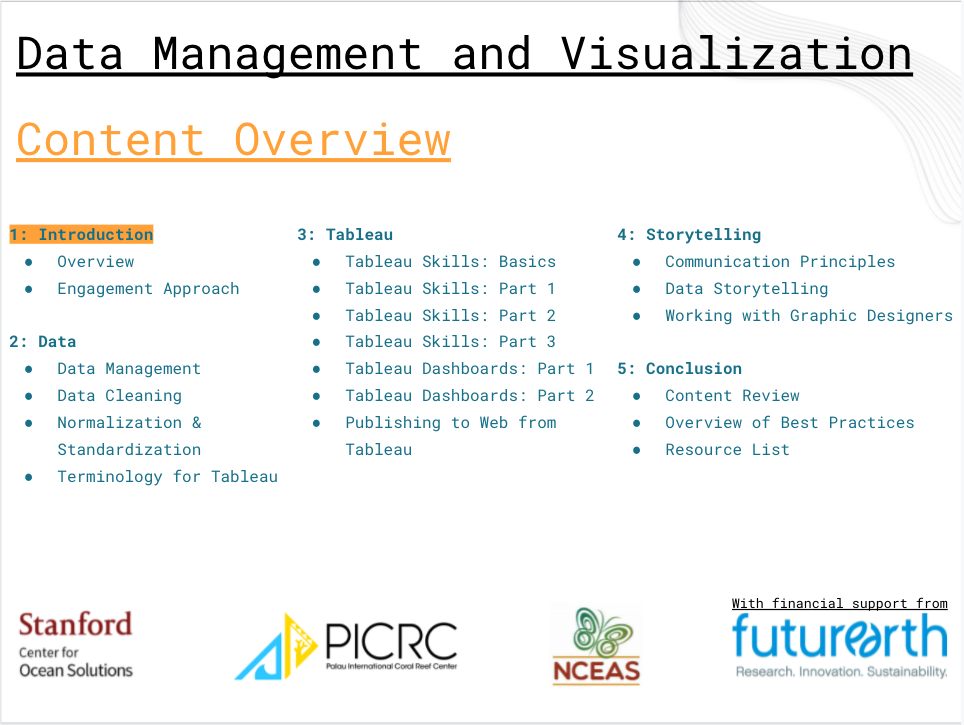
\includegraphics{images/Content_Overview_Intro.png}

\begin{enumerate}
\def\labelenumi{\arabic{enumi}.}
\setcounter{enumi}{3}
\item
  \textbf{\emph{Intended audience:}} In recognizing the wide range of roles and responsibilities individuals may have with respect to data use within an organization, this training is designed to be completed either in a sequence of all material from beginning to end or compartmentalized into modules and sessions to focus on specific skills. Whether you are a data novice interested in learning about all aspects of management and visualization, a data nerd who wants to learn more about visualization and communication, or a communications wizard who wants to be more familiar with data details or skills - this training package includes material to advance your understanding. This content is intended to equip you to better utilize and communicate data stories. In preparation for this course, it may help to briefly consider which data role(s) from the non-exhaustive list below best describes your interests and which lessons best suit your position and needs.
\item
  \textbf{\emph{Required tools:}} To take this training you will need:

  \begin{itemize}
  \tightlist
  \item
    An internet connection, either to download the training booklet and supplementary documents or to view the training through a web browser. Watching the videos in Module 3 on Tableau requires an internet connection.
  \item
    Access to the software Tableau for Module 3. Details on how to install Tableau are in \href{https://nceas.github.io/data-training-picrc-cos/visualizing-data.html\#tableau-basics}{Module 3, Session 1: Tableau Basics} and \href{https://www.tableau.com/products/techspecs\#desktop}{this website} provides details on the necessary operating system requirements to install Tableau.
  \item
    The example data sets for exercises in Modules 2 and 3 are provided as Microsoft Excel files.
  \end{itemize}
\end{enumerate}

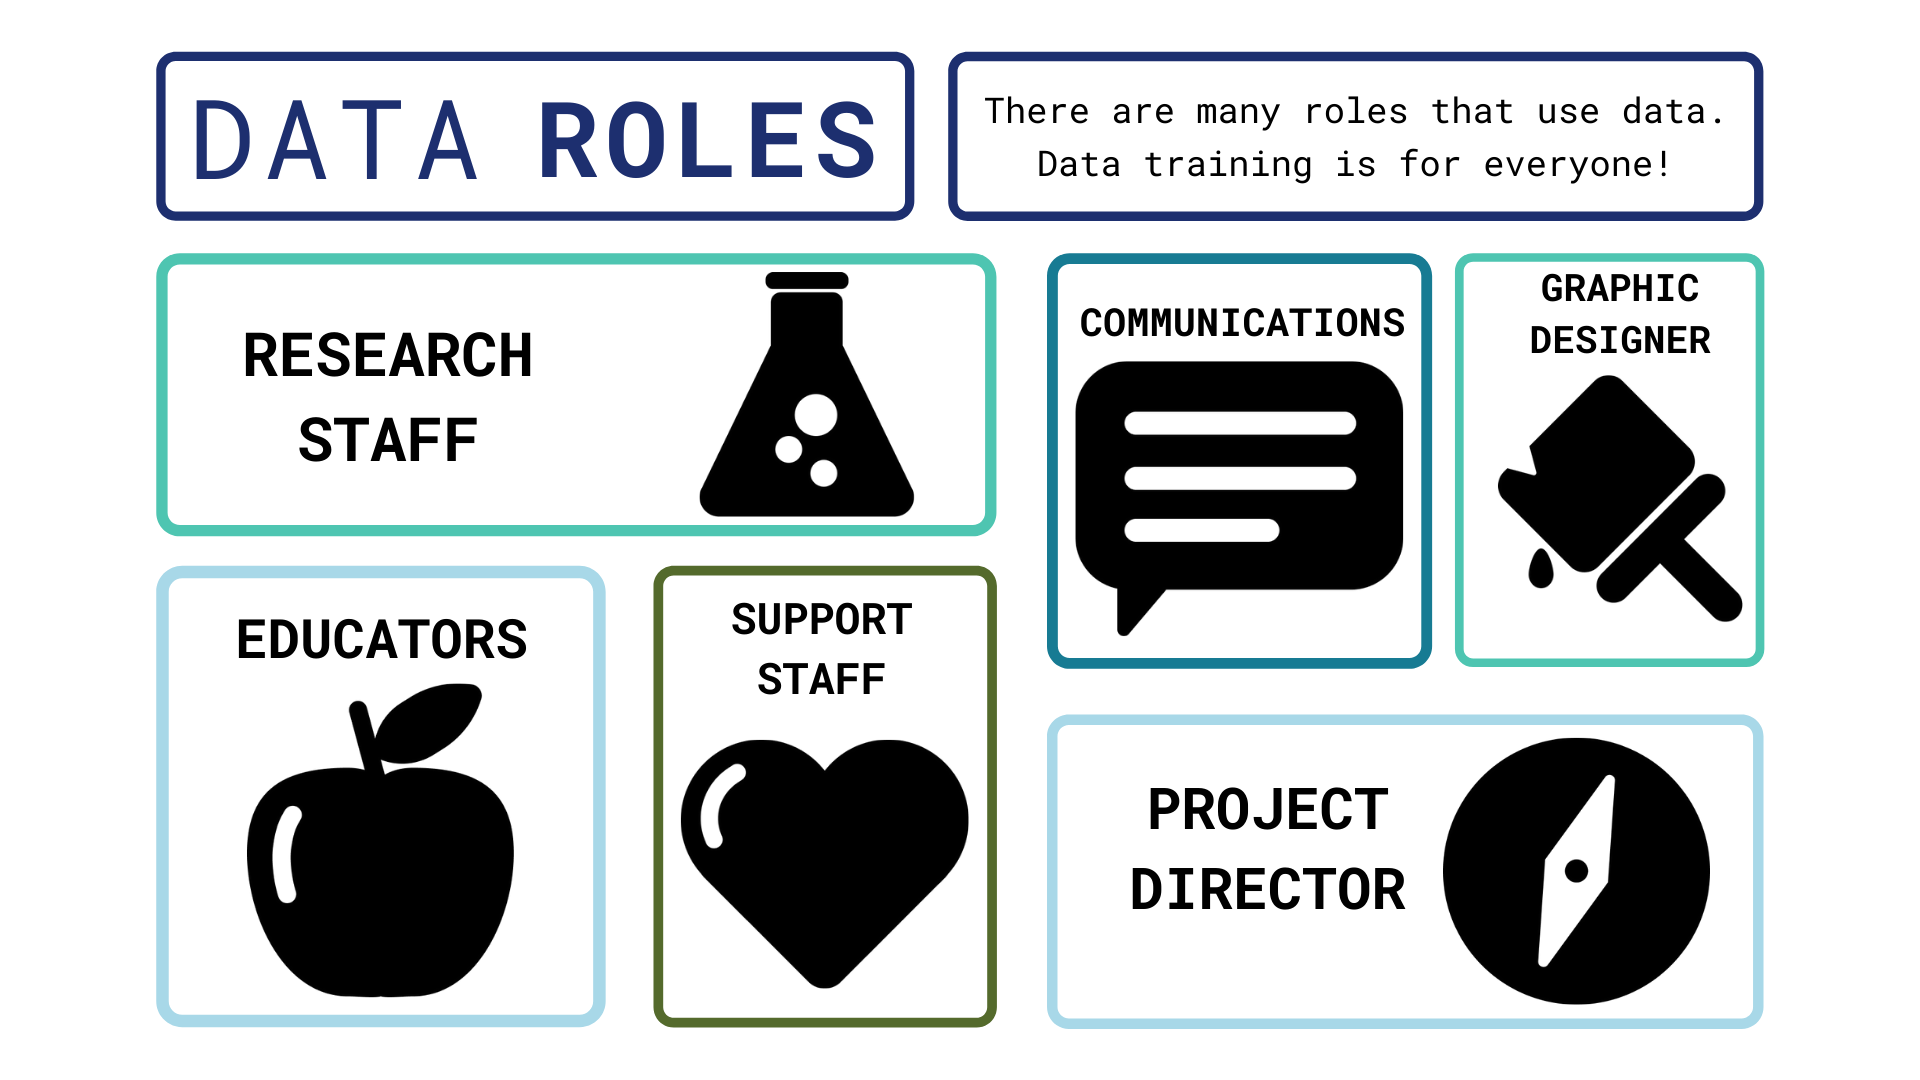
\includegraphics{images/Data_Roles.png}

\begin{enumerate}
\def\labelenumi{\arabic{enumi}.}
\setcounter{enumi}{4}
\tightlist
\item
  \textbf{\emph{Authors:}} This Data Management and Visualization Training package is a collaborative effort amongst researchers and staff from PICRC, NCEAS, and COS. The core contributors to the existing content are recognized below.
\end{enumerate}

\hypertarget{how-to-use-these-materials}{%
\section{How to Use These Materials}\label{how-to-use-these-materials}}

\begin{enumerate}
\def\labelenumi{\arabic{enumi}.}
\item
  \textbf{\emph{Overview:}} The content in the three core modules of this training package targets an audience of researchers or communicators seeking to build their skill set. Each module contains links to additional resources for those that are interested in deeper topical dives.
\item
  \textbf{\emph{Materials:}} Some sessions include distilled handouts or briefs as well as short exercises to help you practice the skills while you are developing them.

  \begin{itemize}
  \tightlist
  \item
    Briefs: Documents that can be utilized as a standalone resource - compiling core messages from a session.
  \item
    Exercises: Self-guided practical work to facilitate learning and enable exploration from a more conceptual framework.
  \item
    Video Tutorials: Recorded lessons (primarily in Module 4: Tableau) providing stepwise guidance to the interface and content.
  \end{itemize}
\item
  \textbf{\emph{Iteration:}} As previously mentioned, the content in this training package is intended to be revisited on an iterative basis as needed. You can proceed through the content in sequence or focus on the modules or sessions of most interest to you. Regardless of your specific data-related role in an organization, there are opportunities to gain greater mastery through iterative practice and collaborative learning.
\item
  \textbf{\emph{Conclusion:}} The concluding module (Module 5) includes a compilation of resources for ``at-a-glance'' skill reminders and references for further investigation.
\end{enumerate}

\hypertarget{working-with-data}{%
\chapter{Working with Data}\label{working-with-data}}

\hypertarget{data-management}{%
\section{Data Management}\label{data-management}}

\textbf{\emph{In this session}}

\begin{enumerate}
\def\labelenumi{\arabic{enumi}.}
\tightlist
\item
  \protect\hyperlink{data-management-learning-objectives}{Learning Objectives}
\item
  \protect\hyperlink{data-management-value-statement}{Value Statement}
\item
  \protect\hyperlink{file-naming}{File naming}
\item
  \protect\hyperlink{creating-a-working-folder-structure}{Creating a Working Folder Structure}
\item
  \protect\hyperlink{metadata}{Metadata}
\item
  \protect\hyperlink{version-control}{Version control}
\item
  \protect\hyperlink{data-management-summary}{Summary}
\end{enumerate}

\hypertarget{data-management-learning-objectives}{%
\subsection{Data Management: Learning objectives}\label{data-management-learning-objectives}}

\begin{enumerate}
\def\labelenumi{\arabic{enumi}.}
\item
  Learn good practices to store, name and keep track of different versions of your data files.
\item
  Understand the importance of metadata and use a template to create your own format.
\end{enumerate}

\hypertarget{data-management-value-statement}{%
\subsection{Data Management: Value statement}\label{data-management-value-statement}}

\begin{enumerate}
\def\labelenumi{\arabic{enumi}.}
\item
  Learning how to properly store, name, and version control your files is the basis to developing systematic procedures to analyze and visualize data.
\item
  Creating metadata files is essential to capturing key information about the context and content of a data file. Every data file should be accompanied by its metadata, which provides data about data. By doing this, you can enable others to better understand your data and work more efficiently.
\end{enumerate}

\hypertarget{file-naming}{%
\subsection{File naming}\label{file-naming}}

\begin{enumerate}
\def\labelenumi{\arabic{enumi}.}
\tightlist
\item
  While there is not a unique way to properly name your files, it is important to be consistent within your organization to help your colleagues recognize which data each file contains. Some of the best practices to do this include:

  \begin{enumerate}
  \def\labelenumii{\arabic{enumii}.}
  \tightlist
  \item
    Use descriptive names that would make sense to any reader. For example, don't use acronyms or abbreviations.
  \item
    Avoid the use of special characters, such as !@\#\$\%\^{}\&*() and others, these are sometimes not supported by some software.
  \item
    Make consistent use of capitalization. Are you going to use capital letters in every word? Maybe only at the beginning of the column name? For example: My\_File1.xlsx vs.~my\_file1.xslx. While none of them is wrong, it is good to choose one format and stick to it
  \item
    Use underscores instead of blank spaces, just as in the example above.
  \item
    If you want to keep track of versions, don't use endings such as ``final'', ``v5'', etc. Instead, we suggest that you either use the date in format YYYYMMDD, or use a version control system, as we will see in a later section.
  \item
    Don't start a file name with a number, though it is fine to use numbers elsewhere in the name, as in the examples above.
  \end{enumerate}
\end{enumerate}

\hypertarget{creating-a-working-folder-structure}{%
\subsection{Creating a working folder structure}\label{creating-a-working-folder-structure}}

\begin{enumerate}
\def\labelenumi{\arabic{enumi}.}
\item
  It is important to create a folder structure that will allow you and your colleagues to easily organize and retrieve any files that you are working with.
\item
  There are some key principles to creating an efficient folder structure:

  \begin{enumerate}
  \def\labelenumii{\arabic{enumii}.}
  \tightlist
  \item
    Store your raw data in its own folder. Every time that you get new data, the first thing you should do is to create a backup by adding it to your raw data folder. This will allow you to always be able to come back to the original file and look for processing errors.
  \item
    Create a separate folder for ``working'' files. These are the files where you will change column names, clean data errors and merge multiple files when necessary. For example, if your team performs annual assessments of reef fish biomass, you may want to store separate files for each year, but combine them in a ``master'' file, which should be located in your ``working'' files folder.
  \item
    Having a consistent file structure across projects, such as folders for script outputs or figures, can make it easier for colleagues and collaborators to understand where to find the files they need.
  \end{enumerate}
\item
  In the example file structure below, each project has its own folder and within each project folder, there are folders for code, data, and output files. The Code folder could store scripts for data cleaning or analysis, the Data folder has subfolders for the raw dataset and a version that has been tidied, and the Output folder could store plots or other results.
\end{enumerate}

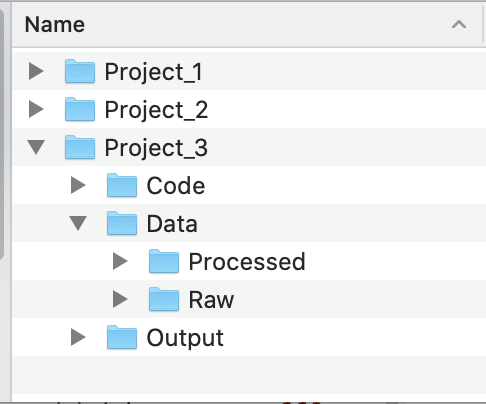
\includegraphics{images/M2S1_example_file_structure.png}

\hypertarget{metadata}{%
\subsection{Metadata}\label{metadata}}

\begin{enumerate}
\def\labelenumi{\arabic{enumi}.}
\item
  Metadata are documentation describing the content, context, and structure of data to enable future interpretation and reuse of the data. Generally, metadata describe who collected the data, what data were collected, when and where they were collected, and why they were collected so that anyone who looks at the data can understand what they mean.
\item
  Along with this class, we provided you with a metadata template, downloadable \href{files/meatadata_template_blank.xlsx}{here}. Please notice that this template can be adjusted to reflect your organization's needs, therefore some of the requested information might change accordingly. Below, you will find an example of a filled out metadata template for the data that we will be using in Module 3.
\item
  Make sure to always share the metadata along with your data files. Some recommendations to do this include:

  \begin{enumerate}
  \def\labelenumii{\arabic{enumii}.}
  \tightlist
  \item
    If working in Excel, create a new tab named ``metadata'' and put the information there
  \item
    If working in other data formats, create a new file with the metadata, store it in the same folder, and name it exactly the same as the data file, adding ``\_metadata'' at the end.
  \end{enumerate}
\end{enumerate}

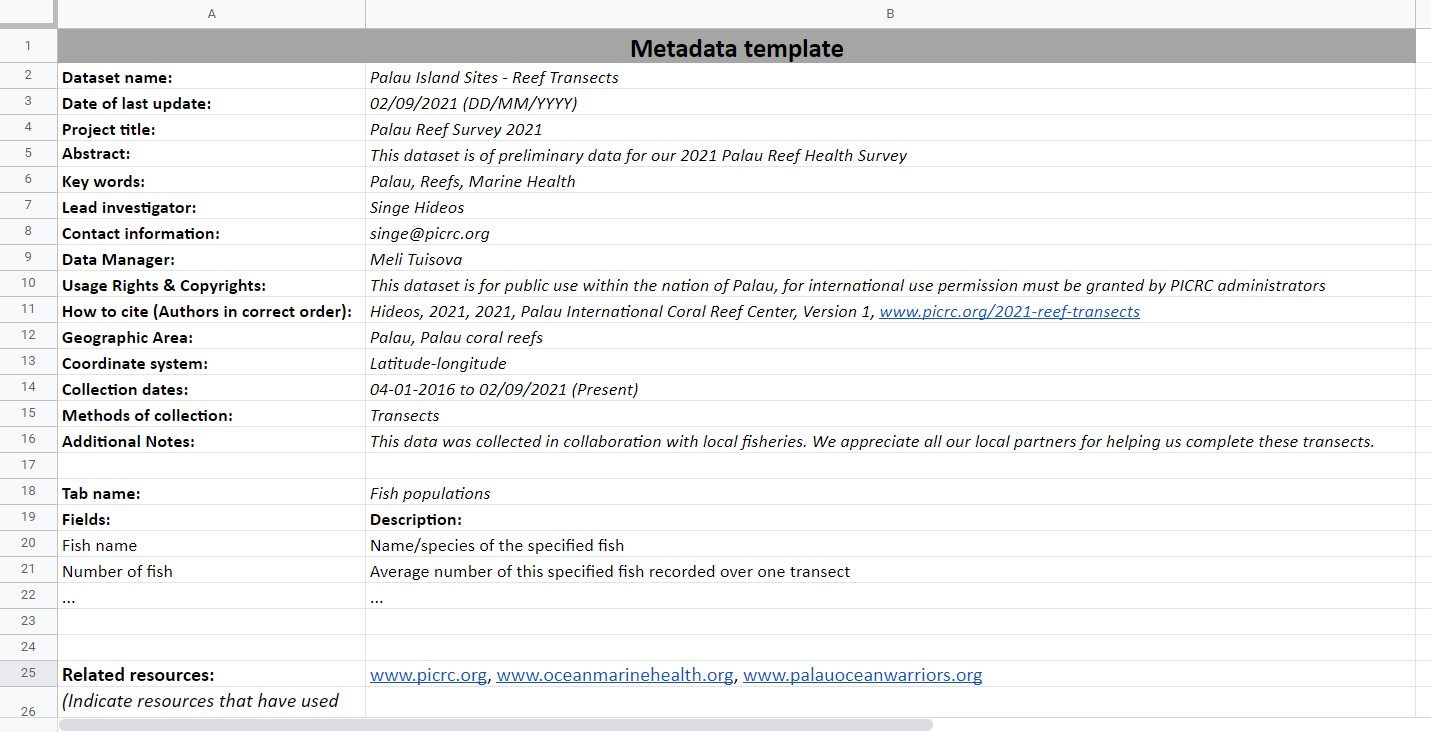
\includegraphics{images/m2s1_metadata_template_filled.jpg}

\hypertarget{version-control}{%
\subsection{Version control}\label{version-control}}

\begin{enumerate}
\def\labelenumi{\arabic{enumi}.}
\tightlist
\item
  Version control is the process of tracking and organizing the changes you make to files over time. Throughout the lifetime of a project, using a system to keep track of different versions of your files and how and why you changed them can make it easier to revert to earlier versions of files or work collaboratively on the same files. Software like \href{https://git-scm.com}{Git} and the associated interface \href{https://github.com}{GitHub} provide a version control framework, particularly useful for code scripts. If you are interested in learning more about Git and GitHub, \href{https://learning.nceas.ucsb.edu/2021-11-RRCourse/version-control-with-git-and-github.html}{this lesson} and these modules (\href{https://learning.nceas.ucsb.edu/2021-11-RRCourse/git-collaboration-and-conflict-management.html}{Git collaboration}, \href{https://learning.nceas.ucsb.edu/2021-11-RRCourse/git-pull-requests-and-branches.html}{Git branches} from a course by NCEAS, focusing on using Git with R, are some starting points. For a broader overview of reproducible science, including the utility of version control, see \href{https://www.nature.com/articles/s41559-017-0160}{this paper} by Lowndes and colleagues.
\end{enumerate}

\hypertarget{data-management-summary}{%
\subsection{Data Management: Summary}\label{data-management-summary}}

\begin{enumerate}
\def\labelenumi{\arabic{enumi}.}
\item
  Well done! Having a good folder structure, file naming practices, and version control capabilities are valuable tools to enable easy collaboration and to streamline workflows.
\item
  Remember that using metadata is extremely important, this is the only way to make sure that you and your team know exactly what is included in a data file. Never share a database without its corresponding metadata.
\end{enumerate}

\hypertarget{data-cleaning}{%
\section{Data Cleaning}\label{data-cleaning}}

\textbf{\emph{In this session }}

\begin{enumerate}
\def\labelenumi{\arabic{enumi}.}
\tightlist
\item
  \protect\hyperlink{data-cleaning-learning-objectives}{Learning objectives}
\item
  \protect\hyperlink{data-cleaning-value-statement}{Value statement}
\item
  \protect\hyperlink{benefits-of-clean-data}{Benefits of clean data}
\item
  \protect\hyperlink{data-types}{Data types}
\item
  \protect\hyperlink{data-cleaning-best-practices}{Best practices}
\item
  \protect\hyperlink{common-cleaning-procedures}{Common cleaning procedures}
\item
  \protect\hyperlink{data-cleaning-summary}{Summary}
\end{enumerate}

\hypertarget{data-cleaning-learning-objectives}{%
\subsection{Data Cleaning: Learning objectives}\label{data-cleaning-learning-objectives}}

\begin{enumerate}
\def\labelenumi{\arabic{enumi}.}
\item
  Learn the benefits of having clean data sets and best practices for organizing and naming in data sheets.
\item
  Learn best practices for cleaning data files.
\end{enumerate}

\hypertarget{data-cleaning-value-statement}{%
\subsection{Data Cleaning: Value statement}\label{data-cleaning-value-statement}}

\begin{enumerate}
\def\labelenumi{\arabic{enumi}.}
\tightlist
\item
  Maintaining clean data sets reduces errors, facilitates searching and analysis, and eases reuse.
\end{enumerate}

\hypertarget{benefits-of-clean-data}{%
\subsection{Benefits of clean data}\label{benefits-of-clean-data}}

\begin{enumerate}
\def\labelenumi{\arabic{enumi}.}
\item
  Let's start by defining what we mean by ``clean data''. Clean data are as consistent, complete, and accurate as possible. Cleaning data is the process of reviewing data sets to standardize formatting, remove duplication, and fix or remove inaccuracies before using or analyzing the data set. Creating clean data sets involves steps in setting up your data organization and in reviewing data before analysis.
\item
  Having clean data has many benefits:

  \begin{itemize}
  \tightlist
  \item
    Reduces errors from redundant updates
  \item
    Enforces data integrity
  \item
    Helps you and future researchers handle large, complex datasets
  \item
    Enables powerful search filtering
  \end{itemize}
\item
  Much has been written on effective data management to enable reuse of data. The following two papers offer words of wisdom:

  \begin{itemize}
  \tightlist
  \item
    \href{https://www.jstor.org/stable/bullecosociamer.90.2.205}{Some simple guidelines for effective data management. Borer et al.~2009. Bulletin of the Ecological Society of America}.
  \item
    \href{https://ojs.library.queensu.ca/index.php/IEE/article/view/4608}{Nine simple ways to make it easier to (re)use your data. White et al.~2013. Ideas in Ecology and Evolution 6}.
  \end{itemize}
\end{enumerate}

\hypertarget{data-types}{%
\subsection{Data types}\label{data-types}}

\begin{enumerate}
\def\labelenumi{\arabic{enumi}.}
\item
  Before we get into cleaning data, let's go over the different ways computers can classify data. The primary data types are

  \begin{itemize}
  \item
    Numeric: integers, decimals

    \begin{itemize}
    \tightlist
    \item
      Any kind of numeric field, except Boolean (binary or true/false statements). Examples include integer, double, floating, etc.
    \end{itemize}
  \item
    Text: strings, including special characters
  \item
    Yes/no, true/false

    \begin{itemize}
    \tightlist
    \item
      Also known as logical or boolean
    \end{itemize}
  \item
    Spatial Location: Coordinates, Country Name, City Name, ZIP code
  \item
    Date and time
  \end{itemize}
\end{enumerate}

\hypertarget{data-cleaning-best-practices}{%
\subsection{Data Cleaning: Best practices}\label{data-cleaning-best-practices}}

\textbf{Data sheet set-up, column names, and data values}

\begin{enumerate}
\def\labelenumi{\arabic{enumi}.}
\item
  In brief, some of the best practices to follow are:

  \begin{itemize}
  \item
    Design your tables to add new observations as rows, not columns. A column should be only one variable and a row should be only one observation.

    \emph{For example, Table 1 below does not follow this design. The highlighted box has information for two types of variables in it and the Observations column has many rows with multiple observations listed. In Table 2, the data has been reentered so that each column has only one data type - see the moved note in orange - and Species column now has only one observation per row.}
    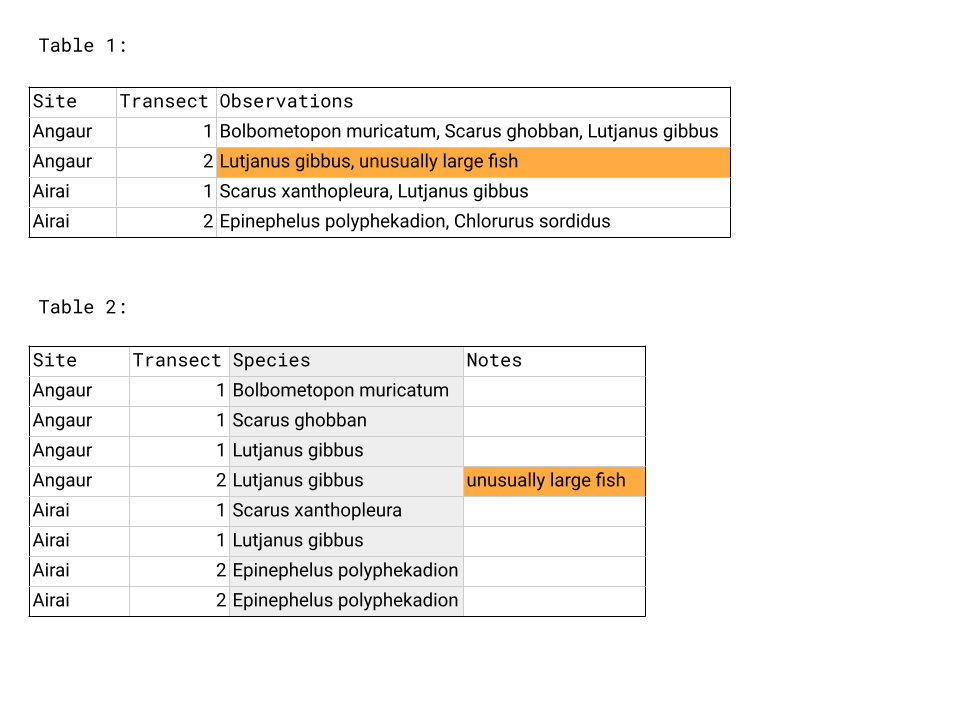
\includegraphics{images/M2S2_image1_observations_in_rows_and_columns.png}
  \item
    Name columns in a clear way that is easy for both people and computers to interpret.

    \begin{itemize}
    \item
      Use descriptive column names that would make sense to any reader. For example, don't use acronyms or abbreviations.
    \item
      Avoid the use of special characters, such as !@\#\$\%\^{}\&*() and others
    \item
      Make consistent use of capitalization. Are you going to use capital letters in every word? Maybe only at the beginning of the column name?
    \item
      Use underscores instead of blank spaces.

      \emph{For example: Number of fish -\textgreater{} Number\_of\_fish}
    \end{itemize}
  \item
    When entering data, make sure there is only one type of value in each column, for example all numeric values or all character strings.
  \item
    As a good practice, we recommend that you and your organization agree on a format and follow it diligently.
  \end{itemize}
\end{enumerate}

\hypertarget{common-cleaning-procedures}{%
\subsection{Common cleaning procedures}\label{common-cleaning-procedures}}

\begin{enumerate}
\def\labelenumi{\arabic{enumi}.}
\item
  When analyzing data, it is important to make sure that there has been a thorough check of the records to ensure that they are as clean and ready as possible. While there is no straightforward way to make sure that all data is clean (given the unique nature of each dataset), there are some guidelines that can be followed.
\item
  This first set of recommendations deals with the overall structure of the database:

  \begin{itemize}
  \item
    Verify that your column names follow the conventions stated in the section above.
  \item
    Verify that there are no empty columns in your dataset, and if there are, eliminate them
  \item
    If you have a column with the date, verify that it is in the right format and that your
    software (e.g., Excel, Access, Tableau) is reading it accordingly.

    \begin{itemize}
    \item
      Word of caution: when working with international collaborators, check the format of dates. Many places use DD/MM/YYYY as the standard date format. The US uses MM/DD/YYYY as the standard date format.
    \item
      Tableau can recognize different date formats. Sometimes it is easier to capture data in 3 separate columns, (year, month, and day), which can then be linked together directly in Tableau.
    \end{itemize}
  \item
    Verify that your database is in long format, as opposed to wide format.

    \begin{itemize}
    \item
      Wide format is a condensed way of presenting data but contains observations in both the column headers and the entered values. Also called block format, wide format is sometimes how data is collected in the field and can be an efficient way of presenting data in a table in a report but is less useful for analysis.
    \item
      In long format, columns only include the type of data and not any information about your actual observations. Having information about your observations in the column headers makes it hard to use that information when analyzing data in Tableau or coding software like R.
    \item
      The same data set often has more rows and fewer columns when in long format compared to wide format, as you can see in the example below. Wide format presents the data efficiently - we can see the whole table - but contains information about the type of meal and type of food in the column headers, which is moved to the rows in long format.
    \end{itemize}
  \end{itemize}
\end{enumerate}

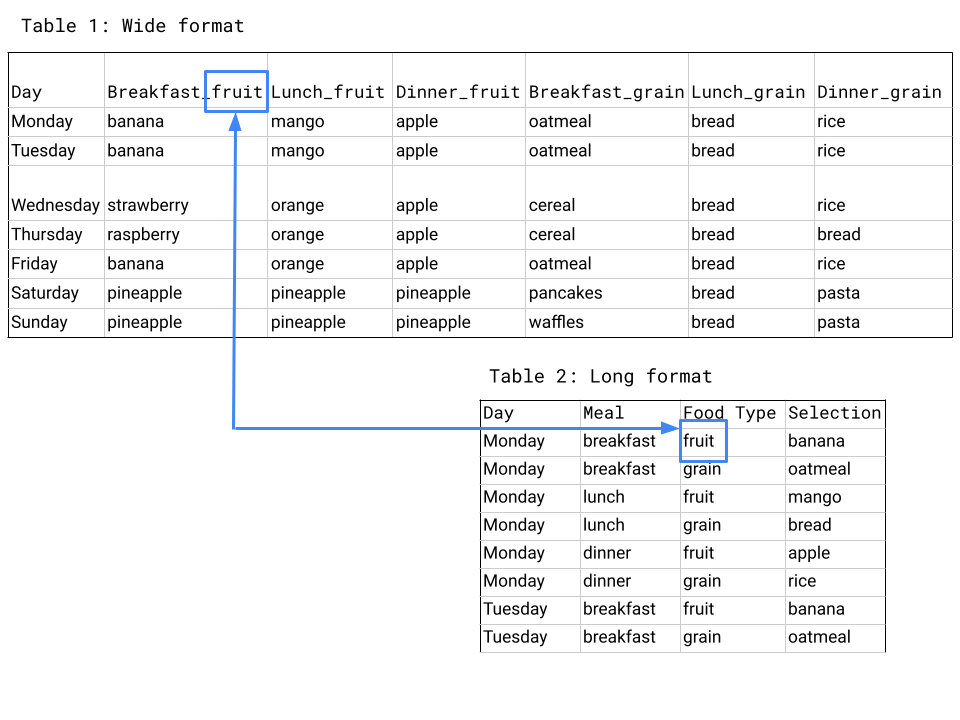
\includegraphics{images/M2S2_image2_long_vs_wide_format.png}

\begin{enumerate}
\def\labelenumi{\arabic{enumi}.}
\setcounter{enumi}{2}
\item
  Next, let's explore some common methods to verify your individual data records:

  \begin{itemize}
  \item
    If the column is numeric:

    \begin{itemize}
    \item
      Verify that there are no text values
    \item
      Plot a histogram with binned values in the x-axis and frequency in the y-axis. If there are very few observations for very low/high values, those are likely outliers or mistakes in the data, like the single high value in the example below. Find them in your raw data and decide whether it is something that you can fix

      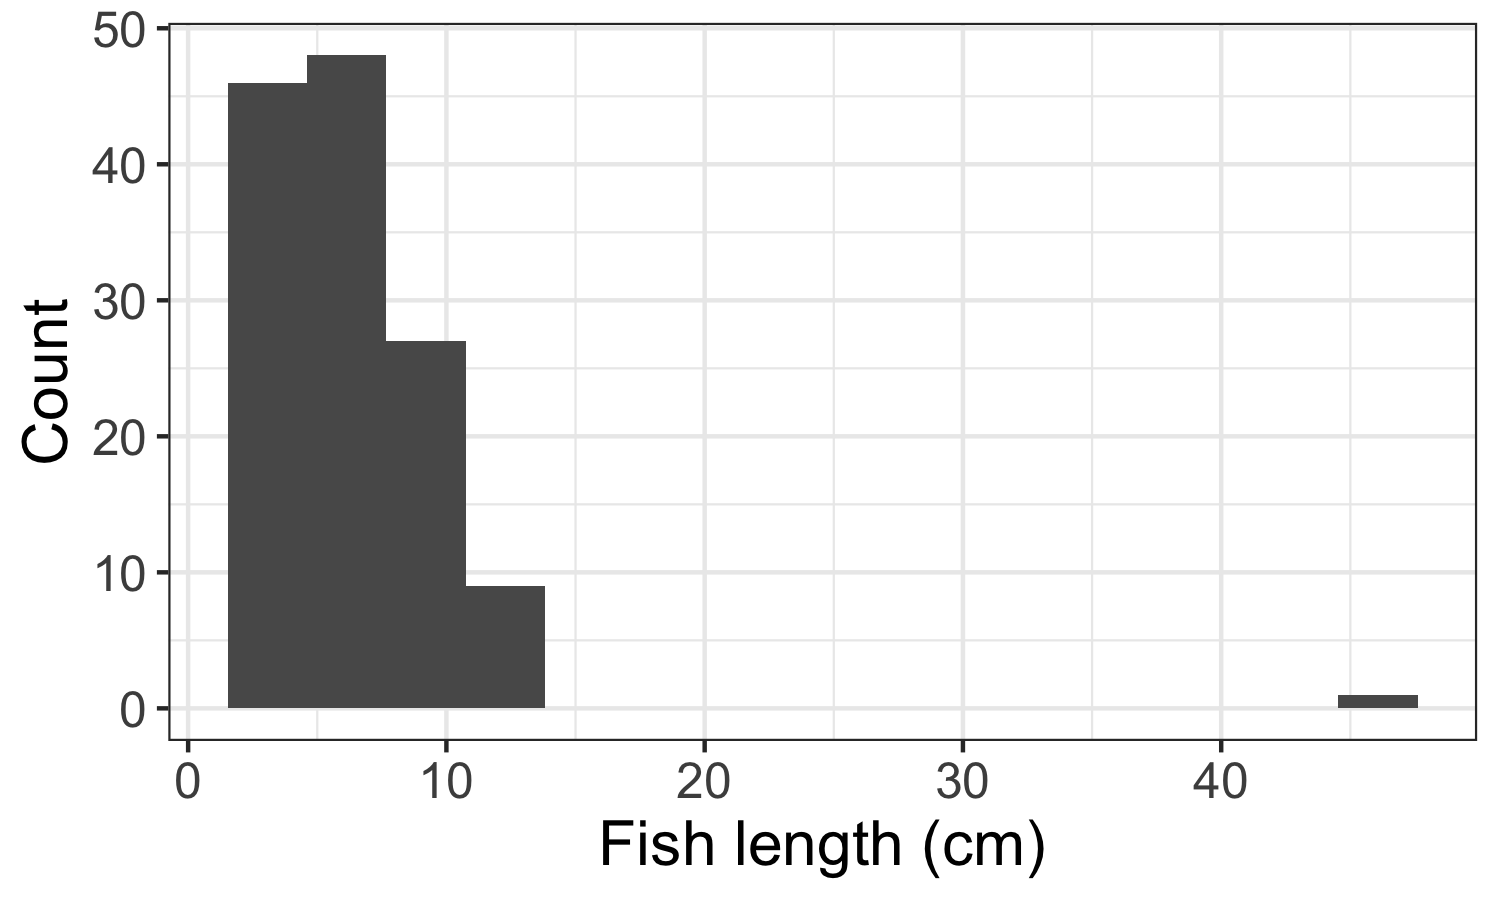
\includegraphics{images/M2S2_image3_data_cleaning_histogram.png}
    \end{itemize}
  \item
    If the column is text:

    \begin{itemize}
    \item
      Verify that there are no numeric values
    \item
      Create a list with all the unique elements and sort them out in alphabetical order. From this list, verify that there are no leading or trailing spaces, misspellings, or typos. Get back to your raw data and correct accordingly.
    \end{itemize}
  \item
    Make sure that you distinguish between values that are zero and data that was not collected. Zeros should be used for values that were measured and found to be zero, for example the number of fish on a transect you swam but saw no fish. Data that was not collected, for example the number of fish you saw at a site you skipped sampling, should be recorded as NA or another symbol you use consistently throughout your data set.
  \end{itemize}
\end{enumerate}

\hypertarget{data-cleaning-summary}{%
\subsection{Data Cleaning: Summary}\label{data-cleaning-summary}}

\begin{enumerate}
\def\labelenumi{\arabic{enumi}.}
\tightlist
\item
  Congratulations! You've now cleaned your data set, storing and presenting it in a way that will be easier to handle, reduce errors, and be easier for others to interpret - both future collaborators and those within your organization. Now that you've cleaned your data set you are ready to start analyzing it.
\end{enumerate}

\hypertarget{normalization-and-standardization}{%
\section{Normalization and Standardization}\label{normalization-and-standardization}}

\textbf{\emph{In This Session}}

\begin{enumerate}
\def\labelenumi{\arabic{enumi}.}
\tightlist
\item
  \protect\hyperlink{normalization-and-standardization-learning-objectives}{Learning objectives}
\item
  \protect\hyperlink{normalization-and-standardization-value-statement}{Value statement}
\item
  \protect\hyperlink{introduction-to-tidy-data}{Introduction to tidy data}
\item
  \protect\hyperlink{normalization}{Normalization}
\item
  \protect\hyperlink{data-organization}{Data organization}
\item
  \protect\hyperlink{standardization}{Standardization}
\item
  \protect\hyperlink{exercise}{Exercise}
\item
  \protect\hyperlink{normalization-and-standardization-summary}{Summary}
\end{enumerate}

\hypertarget{normalization-and-standardization-learning-objectives}{%
\subsection{Normalization and Standardization: Learning objectives}\label{normalization-and-standardization-learning-objectives}}

\begin{enumerate}
\def\labelenumi{\arabic{enumi}.}
\item
  Understand the basics of tidy data, particularly normalization and standardization (the processes of normalization and standardization we refer to here are specific to data management and distinct from the other meanings involving rescaling and recentering data as used in statistics.
\item
  Learn how to design and create effective data tables.
\end{enumerate}

\hypertarget{normalization-and-standardization-value-statement}{%
\subsection{Normalization and Standardization: Value statement}\label{normalization-and-standardization-value-statement}}

\begin{enumerate}
\def\labelenumi{\arabic{enumi}.}
\tightlist
\item
  Normalizing and standardizing data eases analysis and reduces errors. It is also the basis for having datasets that can be easily updated as more data becomes available.
\end{enumerate}

\hypertarget{introduction-to-tidy-data}{%
\subsection{Introduction to tidy data}\label{introduction-to-tidy-data}}

\begin{enumerate}
\def\labelenumi{\arabic{enumi}.}
\item
  Tidy data describes a method of organizing databases and data tables that makes data analysis, searching, and reuse easier.
\item
  The tidy data approach is also known as the relational data model, which is used by relational databases like mySQL, Microsoft Access, and Oracle to store and organize data. If you'd like a more detailed look at the relational data model, see \href{https://learning.nceas.ucsb.edu/2020-11-RRCourse/session-7-data-modeling-essentials.html\#data-modeling-tidy-data}{this lesson} by NCEAS.
\item
  You don't have to have a large and complex data set or be using a relational database, however, to see the benefits of having tidy data!
\end{enumerate}

\hypertarget{normalization}{%
\subsection{Normalization}\label{normalization}}

\begin{enumerate}
\def\labelenumi{\arabic{enumi}.}
\item
  One characteristic of tidy data is normalization - a process of streamlining data structures and reducing redundancy. Normalized data are essentially data in the long format we discussed in the previous session: each column contains only one type of measurement, each row contains one observation, and data are stored in different tables such that each data point only appears once in the database.
\item
  Three practices to keep in mind when designing your tables are:

  \begin{itemize}
  \item
    Add rows, not columns, for new observations.
  \item
    Put values for only one variable in each column.
  \item
    Record each piece of data only once in the database.
  \end{itemize}
\item
  We covered the first two points in the previous session when discussing best practices for designing data tables. The third point addresses how you store your data in different tables and how they interact. To record each piece of data only once in your database, you need to have distinct collections of data stored in different tables that then link to one another.

  \begin{itemize}
  \tightlist
  \item
    As an example of separately storing distinct collections of data, say you visit several sites and do multiple dives at each site. On each dive, you record the fish you see and information about each fish, such as species and length. In this case, you would store information about the sites in one table, information about each dive in another table, and information about the fish recorded on each dive in a third table.

    \begin{itemize}
    \tightlist
    \item
      Storing data only once in a database makes it less likely that there will be errors, especially if you have to alter data later on. For example, if you want to change the format of site coordinates or if the taxonomy of one of the species you sample is updated, you will only have to change entries in one place rather than across multiple tables.
    \item
      After you have normalized your data and identified the relevant tables (e.g., sites, species and dives), there needs to be an identifier that serves as the link between each set of tables. In the example below, the \emph{Dive number} links the Fish info table and the Dive info table - to get information about the dive when analyzing fish, you can pull the data from the Dive info table for the dive of the correct number. Similarly, \emph{Site name} links the Site info table and the Dive info table. The schematic below shows these tables and how they relate.
    \end{itemize}
  \end{itemize}
\end{enumerate}

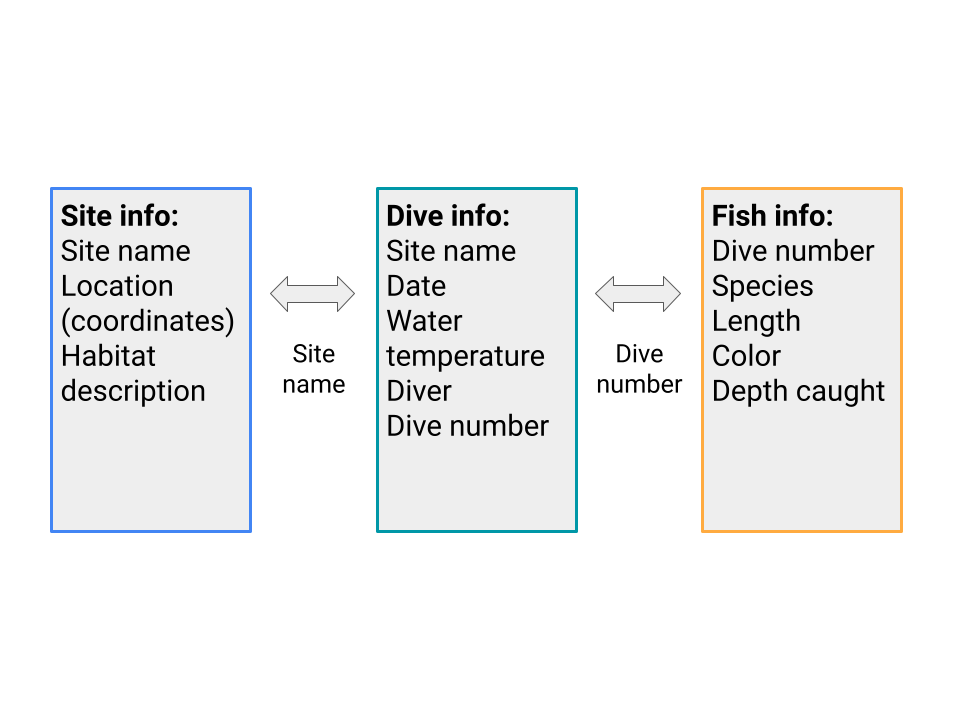
\includegraphics{images/M2S3_normalization_data_tables.png}

\hypertarget{data-organization}{%
\subsection{Data organization}\label{data-organization}}

\begin{enumerate}
\def\labelenumi{\arabic{enumi}.}
\item
  Once you have your data tables normalized, make sure that they are arranged in a way that a computer can easily interpret.

  \begin{itemize}
  \item
    Make sure that each table is stored separately. For example, if you are using a spreadsheet software, each table should hve its own sheet or tab. Multiple tables on the same sheet are hard for software programs like Tableau to read in and understand.
  \item
    Do calculations, like statistics or marginal sums, outside of your data spreadsheet. They are not observations, like the other rows, but rather data analysis.
  \end{itemize}
\end{enumerate}

\hypertarget{standardization}{%
\subsection{Standardization}\label{standardization}}

\begin{enumerate}
\def\labelenumi{\arabic{enumi}.}
\item
  Once you have your data organized in a tidy fashion, it's time to make sure the actual data values are standardized. Standardizing data involves many of the data cleaning steps from the previous session:

  \begin{itemize}
  \item
    Checking that you use consistent entries for the same data values (``Yes'' vs.~``Y'' vs.~``yes'' → choose just one).
  \item
    Checking for data points that are outside the realm of possibility and are likely to be errors, like a dog recorded as weighing 500kg.
  \item
    Verifying that all values within a column are the same data type.
  \end{itemize}
\end{enumerate}

\hypertarget{exercise}{%
\subsection{Exercise}\label{exercise}}

\begin{enumerate}
\def\labelenumi{\arabic{enumi}.}
\tightlist
\item
  Time to practice with an untidy data set! Use what you've learned about data cleaning to normalize and standardize the data set \href{files/M2S2_exercise.xlsx}{here}. See the tidied version \href{files/M2S3_exercise_key.xlsx}{here}.
\end{enumerate}

\hypertarget{normalization-and-standardization-summary}{%
\subsection{Normalization and Standardization: Summary}\label{normalization-and-standardization-summary}}

\begin{enumerate}
\def\labelenumi{\arabic{enumi}.}
\tightlist
\item
  Well done! \href{files/data_processing_checklist.docx}{Here} is a checklist summarizing what we've learned about data organizing and tidying in this module. Now that you've learned about best practices for managing and storing data, it's time to move onto Tableau.
\end{enumerate}

\hypertarget{visualizing-data}{%
\chapter{Visualizing Data}\label{visualizing-data}}

\hypertarget{tableau-basics}{%
\section{Tableau Basics}\label{tableau-basics}}

\textbf{\emph{In this Session}}

\begin{enumerate}
\def\labelenumi{\arabic{enumi}.}
\tightlist
\item
  \protect\hyperlink{tableau-basics-learning-objectives}{Learning Objectives}
\item
  \protect\hyperlink{why-tableau}{Why Tableau?}
\item
  \protect\hyperlink{installing-tableau}{Installing Tableau}
\item
  \protect\hyperlink{user-interface}{User Interface}
\item
  \protect\hyperlink{loading-data}{Loading Data}
\item
  \protect\hyperlink{opening-a-file}{Opening a File}
\item
  \protect\hyperlink{checking-data-types}{Checking Data Types}
\item
  \protect\hyperlink{sheets}{Sheets}
\item
  \protect\hyperlink{tableau-basics-summary}{Summary}
\end{enumerate}

\hypertarget{tableau-basics-learning-objectives}{%
\subsection{Tableau Basics: Learning Objectives}\label{tableau-basics-learning-objectives}}

\begin{enumerate}
\def\labelenumi{\arabic{enumi}.}
\item
  Get familiar with the user interface of Tableau.
\item
  Learn how to connect data sets to Tableau interface.
\end{enumerate}

\hypertarget{why-tableau}{%
\subsection{Why Tableau?}\label{why-tableau}}

\begin{enumerate}
\def\labelenumi{\arabic{enumi}.}
\tightlist
\item
  We are focusing on Tableau for two primary reasons.

  \begin{itemize}
  \tightlist
  \item
    First, Tableau can read a variety of data types, as you will learn in this session. This means that many different software applications and assets can be combined in a single visualization to present to your audience.
  \item
    Second, Tableau is extremely intuitive. Once you get a grasp of the basic skills, you can create compelling visualizations of data in half of the time it would take in other coding software applications.
  \item
    Note: For this training, all the exercises and examples were done with Tableau version 2021.1. The menus may look slightly different in other versions of Tableau.
  \end{itemize}
\end{enumerate}

\hypertarget{installing-tableau}{%
\subsection{Installing Tableau}\label{installing-tableau}}

\begin{enumerate}
\def\labelenumi{\arabic{enumi}.}
\item
  Let's get started with installing the software, to do so, go to
  \url{https://www.tableau.com/} and select ``Try Tableau for Free.''
\item
  Register your email address and username and download the software.
\item
  Once installed, input your key (you get one when you buy the software) and you are ready to go.
\item
  \textbf{Important note:} Tableau offers free 1-year licenses for educational purposes. If you belong to an academic institution, get a free license by going to \url{https://www.tableau.com/community/academic}. Once there, click on ``Free student license''. You will need to provide information about your academic institution to validate your educational license.
\end{enumerate}

\hypertarget{user-interface}{%
\subsection{User Interface}\label{user-interface}}

\begin{enumerate}
\def\labelenumi{\arabic{enumi}.}
\tightlist
\item
  Let's open Tableau! The image below is what you will see the first time you open Tableau. Once you start to save workbooks, they will populate here under \textbf{Open}.
\end{enumerate}

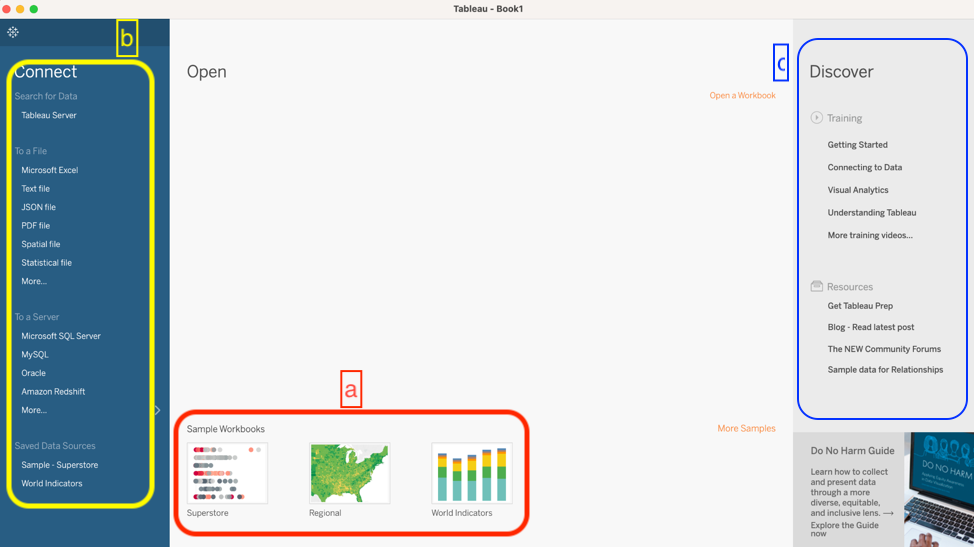
\includegraphics{images/M3S1_image0_User_Interface.png}

\begin{enumerate}
\def\labelenumi{(\alph{enumi})}
\tightlist
\item
  The examples under \textbf{Sample Workbooks} are a great resource for inspiration to see the potential of Tableau.
\item
  This column on the left is where you will load data.
\item
  The \textbf{Training} and \textbf{Resources tabs} are very useful to help you keep learning new skills. If you are interested in investigating or expanding your skills, we recommend starting with the materials in these tabs, rather than searching for other sources on the internet. The materials in these two tabs are very well thought out and provide step-by-step instructions on how to learn new Tableau skills.
\end{enumerate}

\hypertarget{loading-data}{%
\subsection{Loading Data}\label{loading-data}}

\begin{enumerate}
\def\labelenumi{\arabic{enumi}.}
\tightlist
\item
  The most important section of this interface is the \textbf{Connect} menu, where you will load data. There are three main categories of sources that you can load into Tableau.

  \begin{itemize}
  \tightlist
  \item
    \href{https://www.tableau.com/trial/tableau-server?utm_campaign_id=2017049\&utm_campaign=Prospecting-PROD-ALL-ALL-ALL-ALL\&utm_medium=Paid+Search\&utm_source=Bing\&utm_language=EN\&utm_country=USCA\&kw=tableau\%20server\&adgroup=CTX-Brand-Tableau+Server-E\&adused=ETA\&matchtype=e\&placement=\&gclid=c64d924d9b59166571a0f375554410ea\&gclsrc=3p.ds\&msclkid=c64d924d9b59166571a0f375554410ea}{\emph{Tableau Server:}} Data you have saved through your Tableau account. We will not cover that process in this course because most of the users of this training will probably not have a server setup explicitly for Tableau.
  \item
    \emph{Connecting to a local file:} Files from your computer can be Excel files, text files, statistical files, PDFs, and spatial files

    \begin{itemize}
    \tightlist
    \item
      Text files include .csv .doc .log

      \begin{itemize}
      \tightlist
      \item
        You are going to be using \textbf{Text file} frequently if you have .csv (comma separated value) files.
      \end{itemize}
    \item
      Spatial files are commonly referred to as shape files or GIS files. If you have ever dealt with shape files, you might remember that shape files are composed of a \href{https://gisgeography.com/arcgis-shapefile-files-types-extensions/}{few different files} -- some containing the coordinates, metadata, and a table. Tableau has made the adjustments necessary to load one shape file and all the associated files.

      \begin{itemize}
      \tightlist
      \item
        As we will show this later in the course, you can load a shape file and Tableau will display it in a map with just a few clicks.
      \end{itemize}
    \end{itemize}
  \item
    \emph{Connecting to a server:} You can connect to services that are online like Google Sheets, or Microsoft Office 365.

    \begin{itemize}
    \tightlist
    \item
      One of the benefits of using this approach is that when you modify the original file, the modifications will be directly updated in Tableau.

      \begin{itemize}
      \tightlist
      \item
        Let's say you created a report with nice graphs in 2020 because that's the data that you had when you created the report and then in 2021 you edited your Google sheet. The next time you open your Tableau workbook, all the data will be updated and contain the new data from 2021.
      \end{itemize}
    \end{itemize}
  \end{itemize}
\item
  It's very important to make sure that you organize and manage your files such that you know exactly where your files are. Keep in mind that if you connect to a server, any changes that you make in the original file will have an impact on how your visualization looks in Tableau.
\end{enumerate}

\hypertarget{opening-a-file}{%
\subsection{Opening a file}\label{opening-a-file}}

\begin{enumerate}
\def\labelenumi{\arabic{enumi}.}
\item
  Create a new folder on your desktop. Name the folder ``Tableau Data Training.''
\item
  Download this file: \href{files/CRM_Fish_edit.xlsx}{CRM\_Fish\_edit} and save it in the ``Tableau Data Training'' folder.
\item
  Follow along with this video to connect the new data file to Tableau.
\end{enumerate}

\begin{enumerate}
\def\labelenumi{\arabic{enumi}.}
\setcounter{enumi}{3}
\tightlist
\item
  Progress check-in. So far, you have:

  \begin{itemize}
  \tightlist
  \item
    Downloaded an excel file and connected it to Tableau
  \item
    In Tableau, you learned about drag and drop. As Alfredo always says, ``Tableau is all about drag and drop.''
  \item
    You connected the two tabs CRM\_Fish and CRM\_Site within the CRM\_fish\_edit Excel file---now in the Tableau interface. There is an orange line showing the connection.
  \end{itemize}
\end{enumerate}

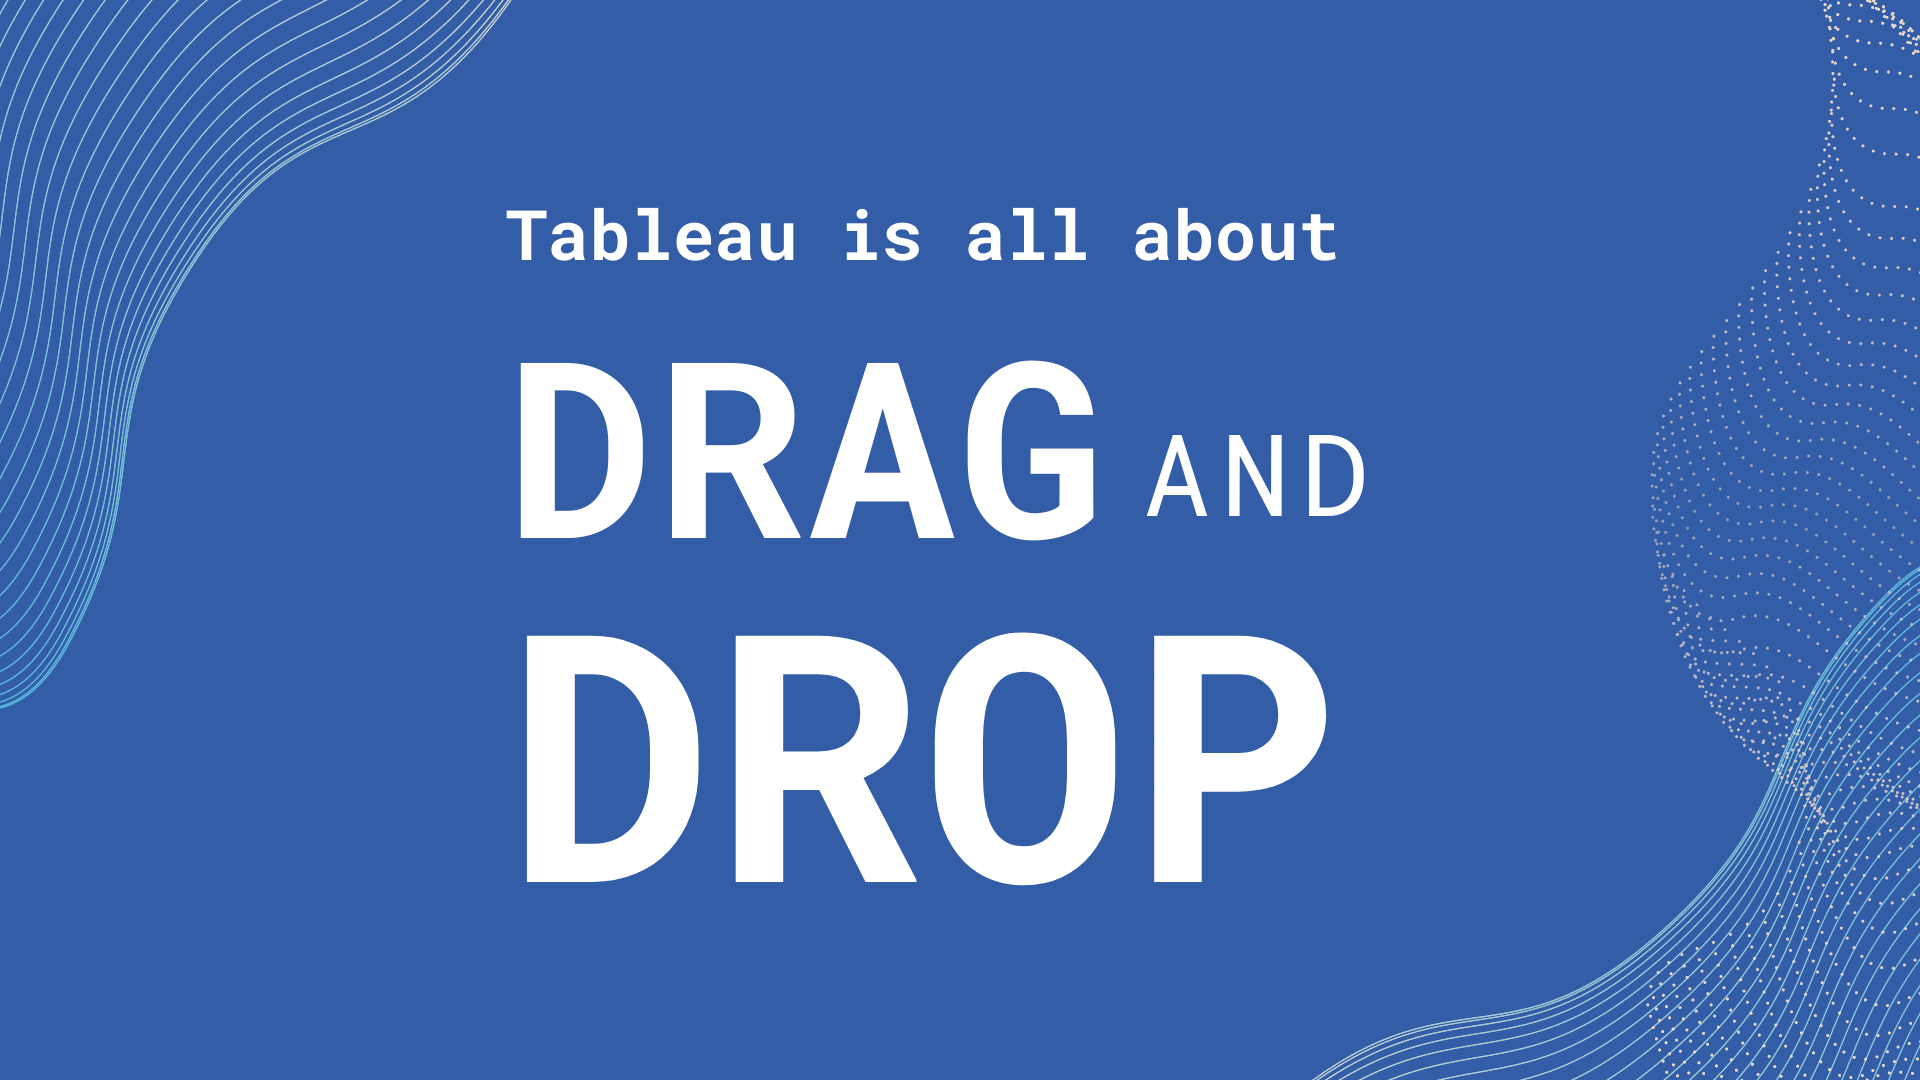
\includegraphics{images/M3S1_image1_draganddrop.png}

\hypertarget{checking-data-types}{%
\subsection{Checking Data Types}\label{checking-data-types}}

\begin{enumerate}
\def\labelenumi{\arabic{enumi}.}
\tightlist
\item
  When you load a data file, you have to check that Tableau properly labels the data types. Here, we will discuss what those data types are and how they are assigned in Tableau.

  \begin{itemize}
  \tightlist
  \item
    \textbf{\emph{Dimensions and Measurements}}

    \begin{itemize}
    \tightlist
    \item
      \textbf{Dimension} (also referred to as factor) is any information that is defined a priori of your actual sampling and helps to describe or categorize your results. Whenever you can call something a category it is a factor. Depending on your data, factors are sometimes written as numbers, like year or site ID.

      \begin{itemize}
      \tightlist
      \item
        Example: Site name, species, habitat
      \end{itemize}
    \item
      \textbf{Measurements} are the actual results of your sampling. They are usually numbers that you went into the field to measure.

      \begin{itemize}
      \tightlist
      \item
        Example: Fish size, population count, temperature
      \end{itemize}
    \item
      Tricky Case: Coordinates

      \begin{itemize}
      \tightlist
      \item
        Coordinates are a factor when you already know the coordinates where you are going to take your sample. Example: You have ten sites that you visit each year to count the number of whales. The coordinates of each site are a factor because they are predetermined. You know where you are going to gather data each time.
      \item
        Coordinates are a measurement when it is part of the information that you are recording and it is not predefined. Example: you put a gps tracker on a whale and every time the whale surfaces, you record the coordinates. You did not know ahead of time where the whale would surface and the location is what the study is measuring.
      \end{itemize}
    \item
      Tricky case: Is depth a factor or a measurement?

      \begin{itemize}
      \tightlist
      \item
        Depth is a factor when indicating a transect location. Example: If you are always putting transects at either 3m or 30m you can categorize depth into shallow or deep.
      \item
        Depth is a measurement when it is recorded with every observation. Example: If you are swimming for 50 minutes to record visual observations of fish while also noting the depth at each observation, then depth is also a measurement. You measured and recorded your depth as you recorded the observation of the fish.
      \end{itemize}
    \item
      Practice exercise: Time

      \begin{itemize}
      \tightlist
      \item
        SCENARIO 1: Let's say that you are birdwatching and you want to know what time of day birds are more active. You count the birds and you write down the time that you saw each bird. Is time a measurement or a factor?

        \begin{itemize}
        \tightlist
        \item
          Answer: Measurement because you are registering the time every time you see a bird.
        \end{itemize}
      \item
        SCENARIO 2: You want to know whether there are more birds in the morning, the afternoon, or in the evening.

        \begin{itemize}
        \tightlist
        \item
          Answer: In this case, time is a factor because you go out three times a day, you count all the birds you see at that time and categorize by morning, afternoon, or evening.
        \end{itemize}
      \end{itemize}
    \end{itemize}
  \item
    \textbf{\emph{Types of Data}}

    \begin{itemize}
    \tightlist
    \item
      Different ways computers classify data:

      \begin{itemize}
      \tightlist
      \item
        Numeric - integers, decimals

        \begin{itemize}
        \tightlist
        \item
          Any kind of numeric field, except Boolean (binary or true/false statements). Examples include integer, double, floating, etc.
        \end{itemize}
      \item
        Text - strings, including special characters
      \item
        Yes/no, true/false - Also known as logical or boolean
      \item
        Spatial Location - Coordinates, Country Name, City Name, ZIP code
      \item
        Date and time. Tableau can recognize different date formats. One best practice is to separate fields for year, month, and day, which can be linked together directly in Tableau.
      \end{itemize}
    \end{itemize}
  \item
    \textbf{\emph{Discrete and Continuous Data}}

    \begin{itemize}
    \tightlist
    \item
      \textbf{Discrete data} refer to variables that can only be conceptualized in a unitary manner. \emph{It is quite similar to the difference between using many vs much. In this case, discrete data would be for things described as many}.

      \begin{itemize}
      \tightlist
      \item
        Example for text -- color, name, city
      \item
        Example for numbers -- number of transects conducted, position in a ranking
      \end{itemize}
    \item
      \textbf{Continuous data} refer to variables that cannot be counted by units, but instead as continuous amounts. \emph{Following the example above, continuous data would be for things described as much}.

      \begin{itemize}
      \tightlist
      \item
        Example: number of fish recorded, total biomass, height, depth
      \end{itemize}
    \end{itemize}
  \end{itemize}
\item
  You should go through the preview of the data and ensure that each column is labeled correctly.

  \begin{itemize}
  \tightlist
  \item
    \emph{Note: Never skip this step even if you have worked with the data set in Tableau before!}
  \end{itemize}
\item
  The type of data is shown as symbols above the column title.
\end{enumerate}

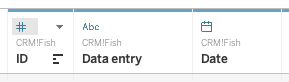
\includegraphics{images/m3s1_image2_Data-Type-Symbols.png}

\begin{enumerate}
\def\labelenumi{\arabic{enumi}.}
\setcounter{enumi}{3}
\item
  As you can see, the \textbf{ID} column is correctly labeled as a number; \textbf{Data entry} is a string (or text); and \textbf{Date} is a date (little calendar symbol).

  \begin{itemize}
  \tightlist
  \item
    \emph{Note: Remember string is a synonym for text in Tableau.}
  \end{itemize}
\item
  To change the label, click on the symbol and a drop-down menu will appear.

  \begin{itemize}
  \tightlist
  \item
    The \textbf{CRM\_Fish} table should look like this:
  \end{itemize}

  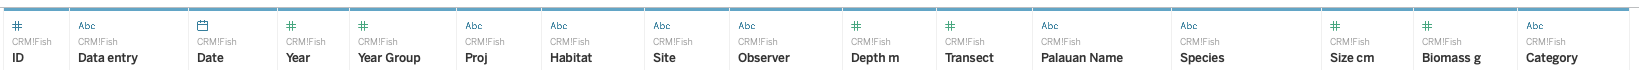
\includegraphics{images/m3s1_image3_CRM_Fish-Data-Types.png}

  \begin{itemize}
  \tightlist
  \item
    The \textbf{CMR\_Site} table should look like this:
  \end{itemize}

  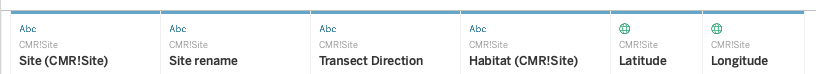
\includegraphics{images/m3s1_image4_CMR_Site-Data-Types.png}

  \begin{itemize}
  \tightlist
  \item
    Notice that Latitude and Longitude are spatial data. If you open the drop-down, you will see that you can specify the type of spatial data provided under Geographic Role.\\
    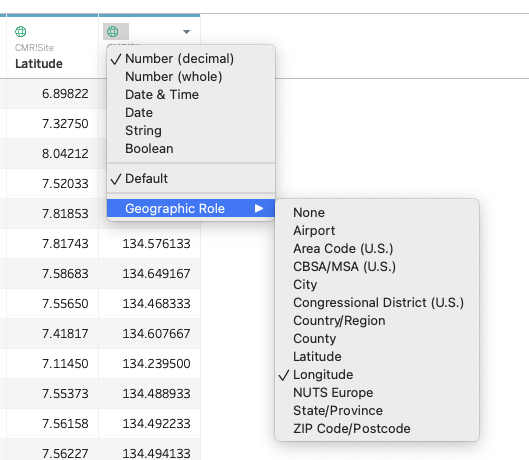
\includegraphics{images/m3s1_image5_Data_Types_choosing-coordinates.png}
  \end{itemize}
\end{enumerate}

\hypertarget{sheets}{%
\subsection{Sheets}\label{sheets}}

\begin{enumerate}
\def\labelenumi{\arabic{enumi}.}
\tightlist
\item
  Sheets Cheat Sheet

  \begin{itemize}
  \tightlist
  \item
    Discrete vs.~Continuous

    \begin{itemize}
    \tightlist
    \item
      {DISCRETE is Blue}
    \item
      {CONTINUOUS is Green}
    \end{itemize}
  \item
    Factors vs.~Measures

    \begin{itemize}
    \tightlist
    \item
      Above the grey line is a FACTOR
    \item
      Below the grey line is a MEASURE
    \end{itemize}
  \end{itemize}
\end{enumerate}

\hypertarget{tableau-basics-summary}{%
\subsection{Tableau Basics Summary}\label{tableau-basics-summary}}

\begin{enumerate}
\def\labelenumi{\arabic{enumi}.}
\tightlist
\item
  Great job! You have completed your first in depth Tableau session. Now, you know how to explore Tableau's user interface, to connect a data file, check data types, and open sheets.
\end{enumerate}

\hypertarget{tableau-skills-part-1-basic-plots-with-single-variables}{%
\section{Tableau Skills Part 1: Basic plots with single variables}\label{tableau-skills-part-1-basic-plots-with-single-variables}}

\textbf{\emph{In this Session}}

\begin{enumerate}
\def\labelenumi{\arabic{enumi}.}
\tightlist
\item
  \protect\hyperlink{basic-plots-learning-objectives}{Learning Objectives}
\item
  \protect\hyperlink{basic-plots-value-statement}{Value Statement}
\item
  \protect\hyperlink{creating-your-first-graph}{Creating Your First Graph}
\item
  \protect\hyperlink{basic-plots-using-the-marks-menu}{Basic Plots using the Marks Menu}
\item
  \protect\hyperlink{line-plot}{Line Plot}
\item
  \protect\hyperlink{area-plot}{Area Plot}
\item
  \protect\hyperlink{map}{Map}
\item
  \protect\hyperlink{bubble-plot}{Bubble Plot}
\item
  \protect\hyperlink{scatter-plot}{Scatter Plot}
\item
  \protect\hyperlink{editing-and-formatting-the-axes}{Editing and Formatting the Axes}
\item
  \protect\hyperlink{saving-my-files}{Saving my Files}
\item
  \protect\hyperlink{homework-exercise}{Homework Exercise}
\item
  \protect\hyperlink{tableau-skills-part-1-summary}{Summary}
\end{enumerate}

\hypertarget{basic-plots-learning-objectives}{%
\subsection{Basic Plots: Learning Objectives}\label{basic-plots-learning-objectives}}

\begin{enumerate}
\def\labelenumi{\arabic{enumi}.}
\item
  Explore the user interface.
\item
  Learn how to make basic plots and customize them.
\item
  Learn how to save and share workbooks.
\end{enumerate}

\hypertarget{basic-plots-value-statement}{%
\subsection{Basic Plots: Value Statement}\label{basic-plots-value-statement}}

\begin{enumerate}
\def\labelenumi{\arabic{enumi}.}
\item
  Learning how to make basic plots in Tableau (e.g., bars, lines, pies, etc.) and how to take full control of the appearance will prepare you to take full advantage of Tableau's more advanced skills.
\item
  \emph{For this session we recommend that, if possible, you have two screens open---one with Tableau and one with the course material---so you can follow along with the exercises.}
\end{enumerate}

\hypertarget{creating-your-first-graph}{%
\subsection{Creating your first graph}\label{creating-your-first-graph}}

\begin{enumerate}
\def\labelenumi{\arabic{enumi}.}
\tightlist
\item
  In the menu on the left, find \textbf{Habitat} under CRM\_Fish
\end{enumerate}

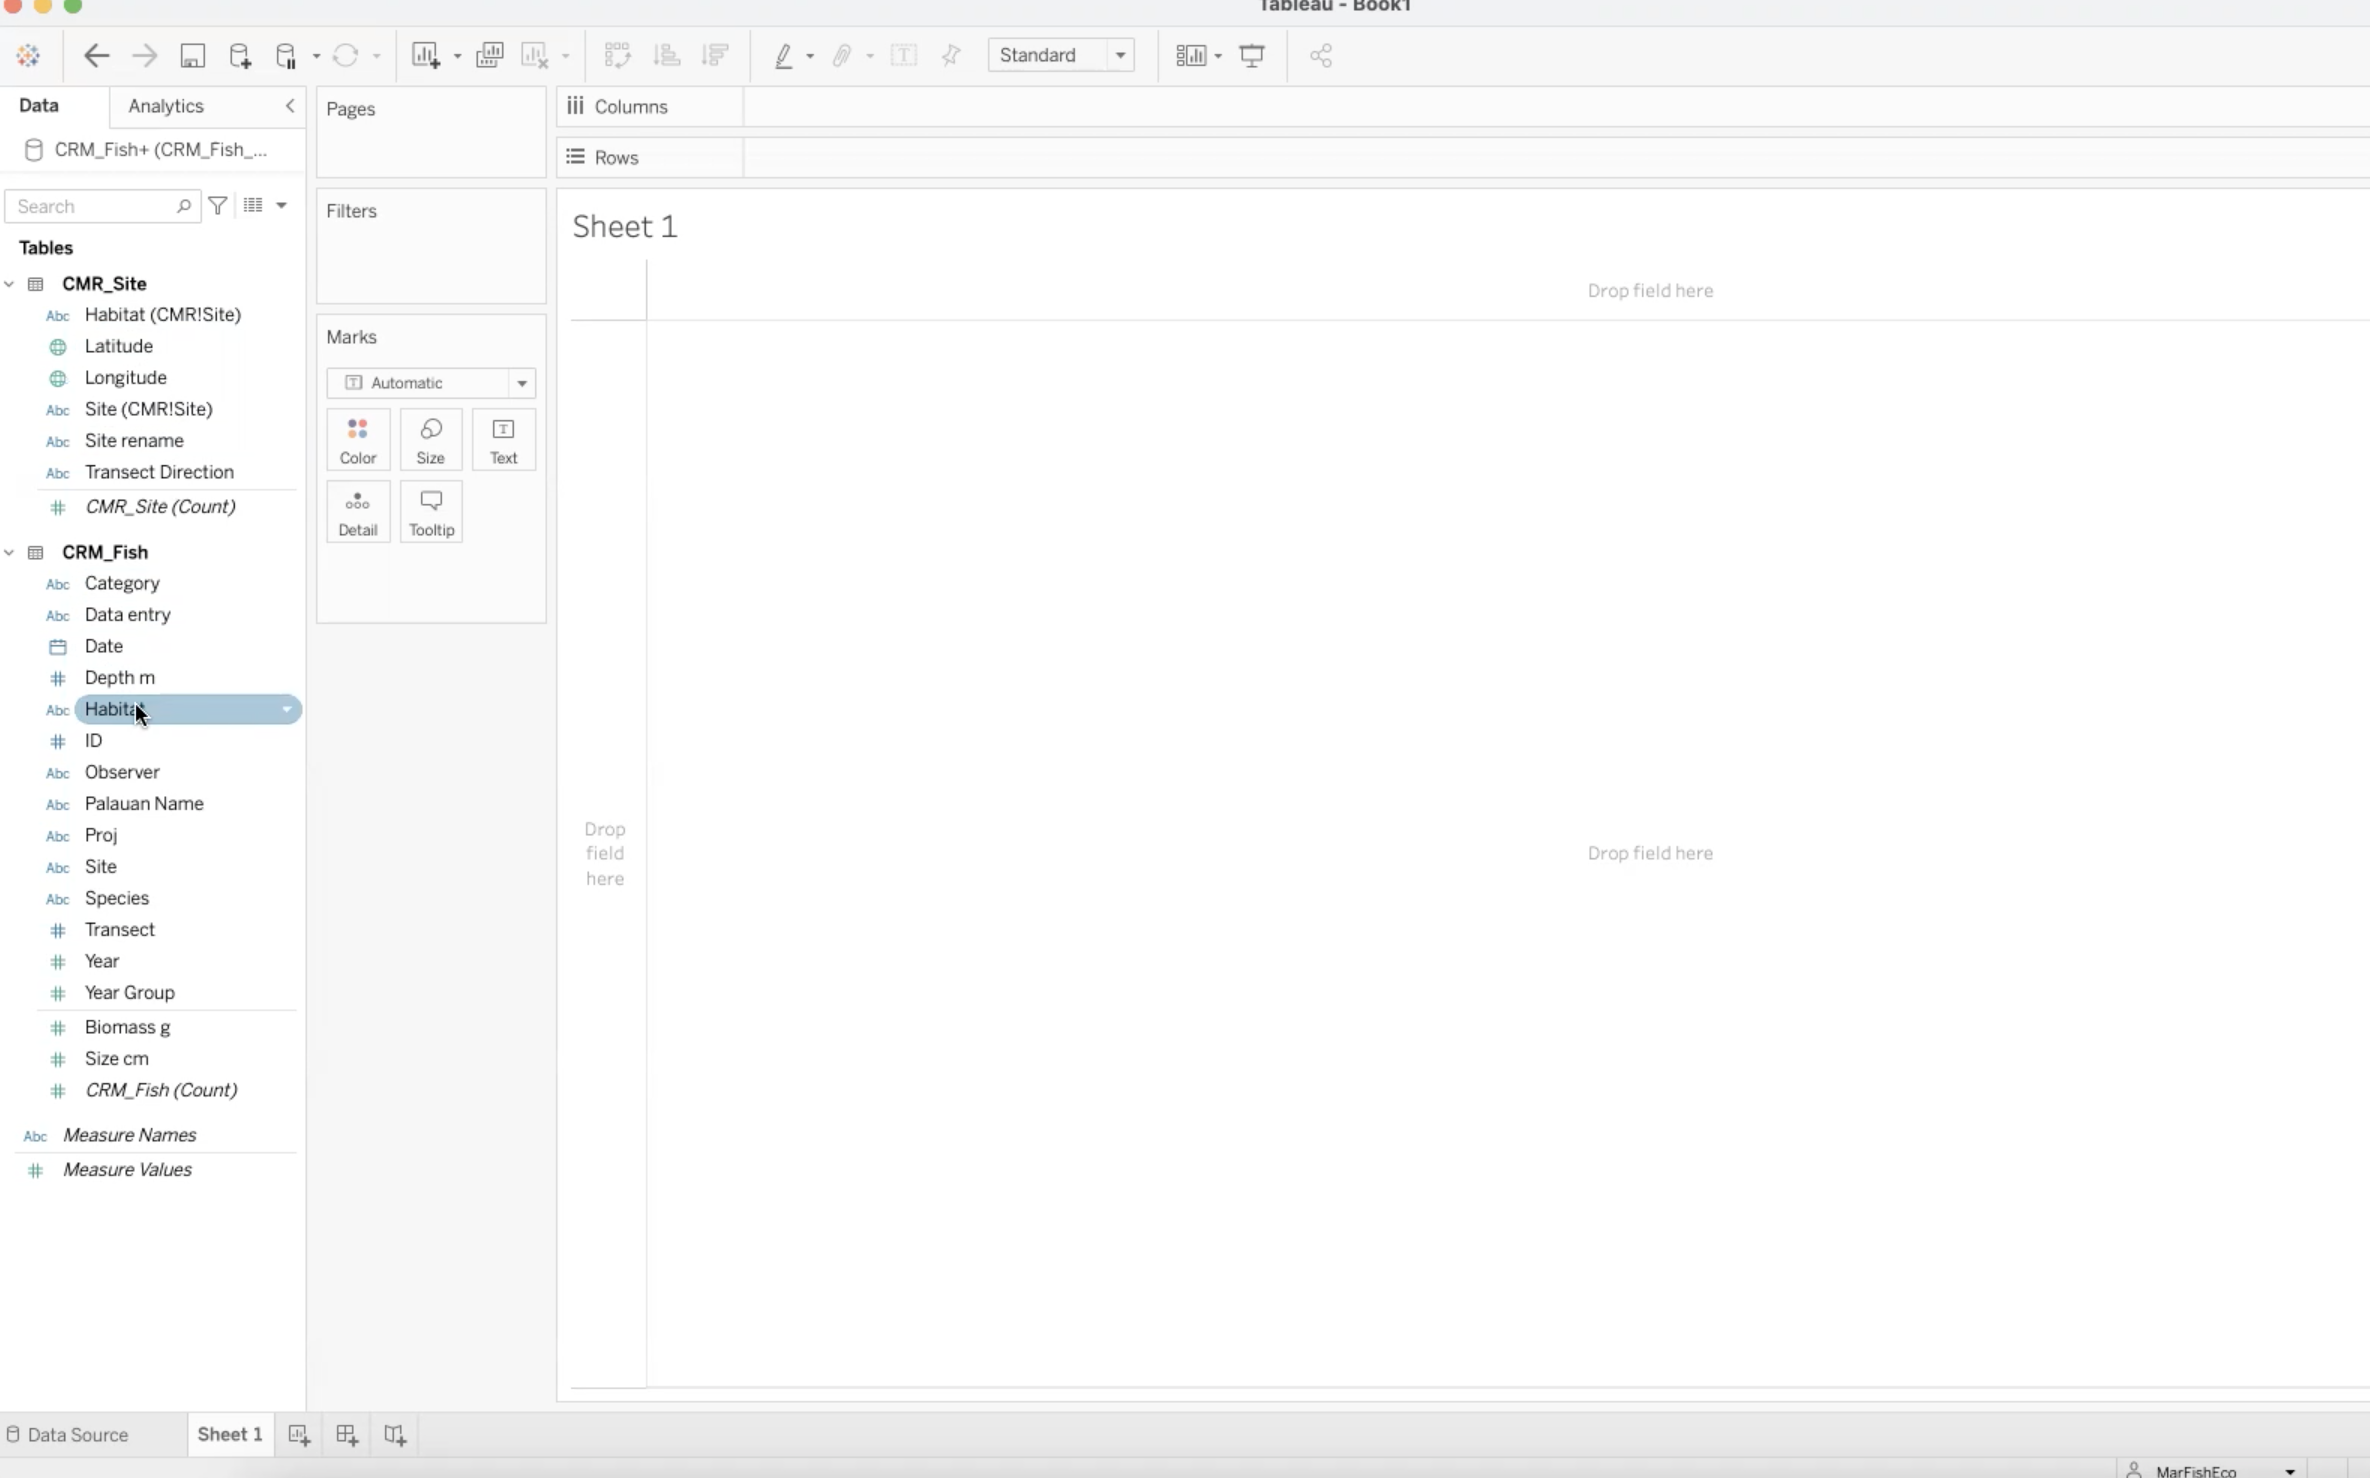
\includegraphics{images/M3S2_find-habitat.png}

\begin{enumerate}
\def\labelenumi{\arabic{enumi}.}
\setcounter{enumi}{1}
\tightlist
\item
  Drag and drop \textbf{Habitat} into \textbf{Columns}

  \begin{itemize}
  \tightlist
  \item
    This will place \textbf{Habitat} in the x-axis of the graph
  \end{itemize}
\end{enumerate}

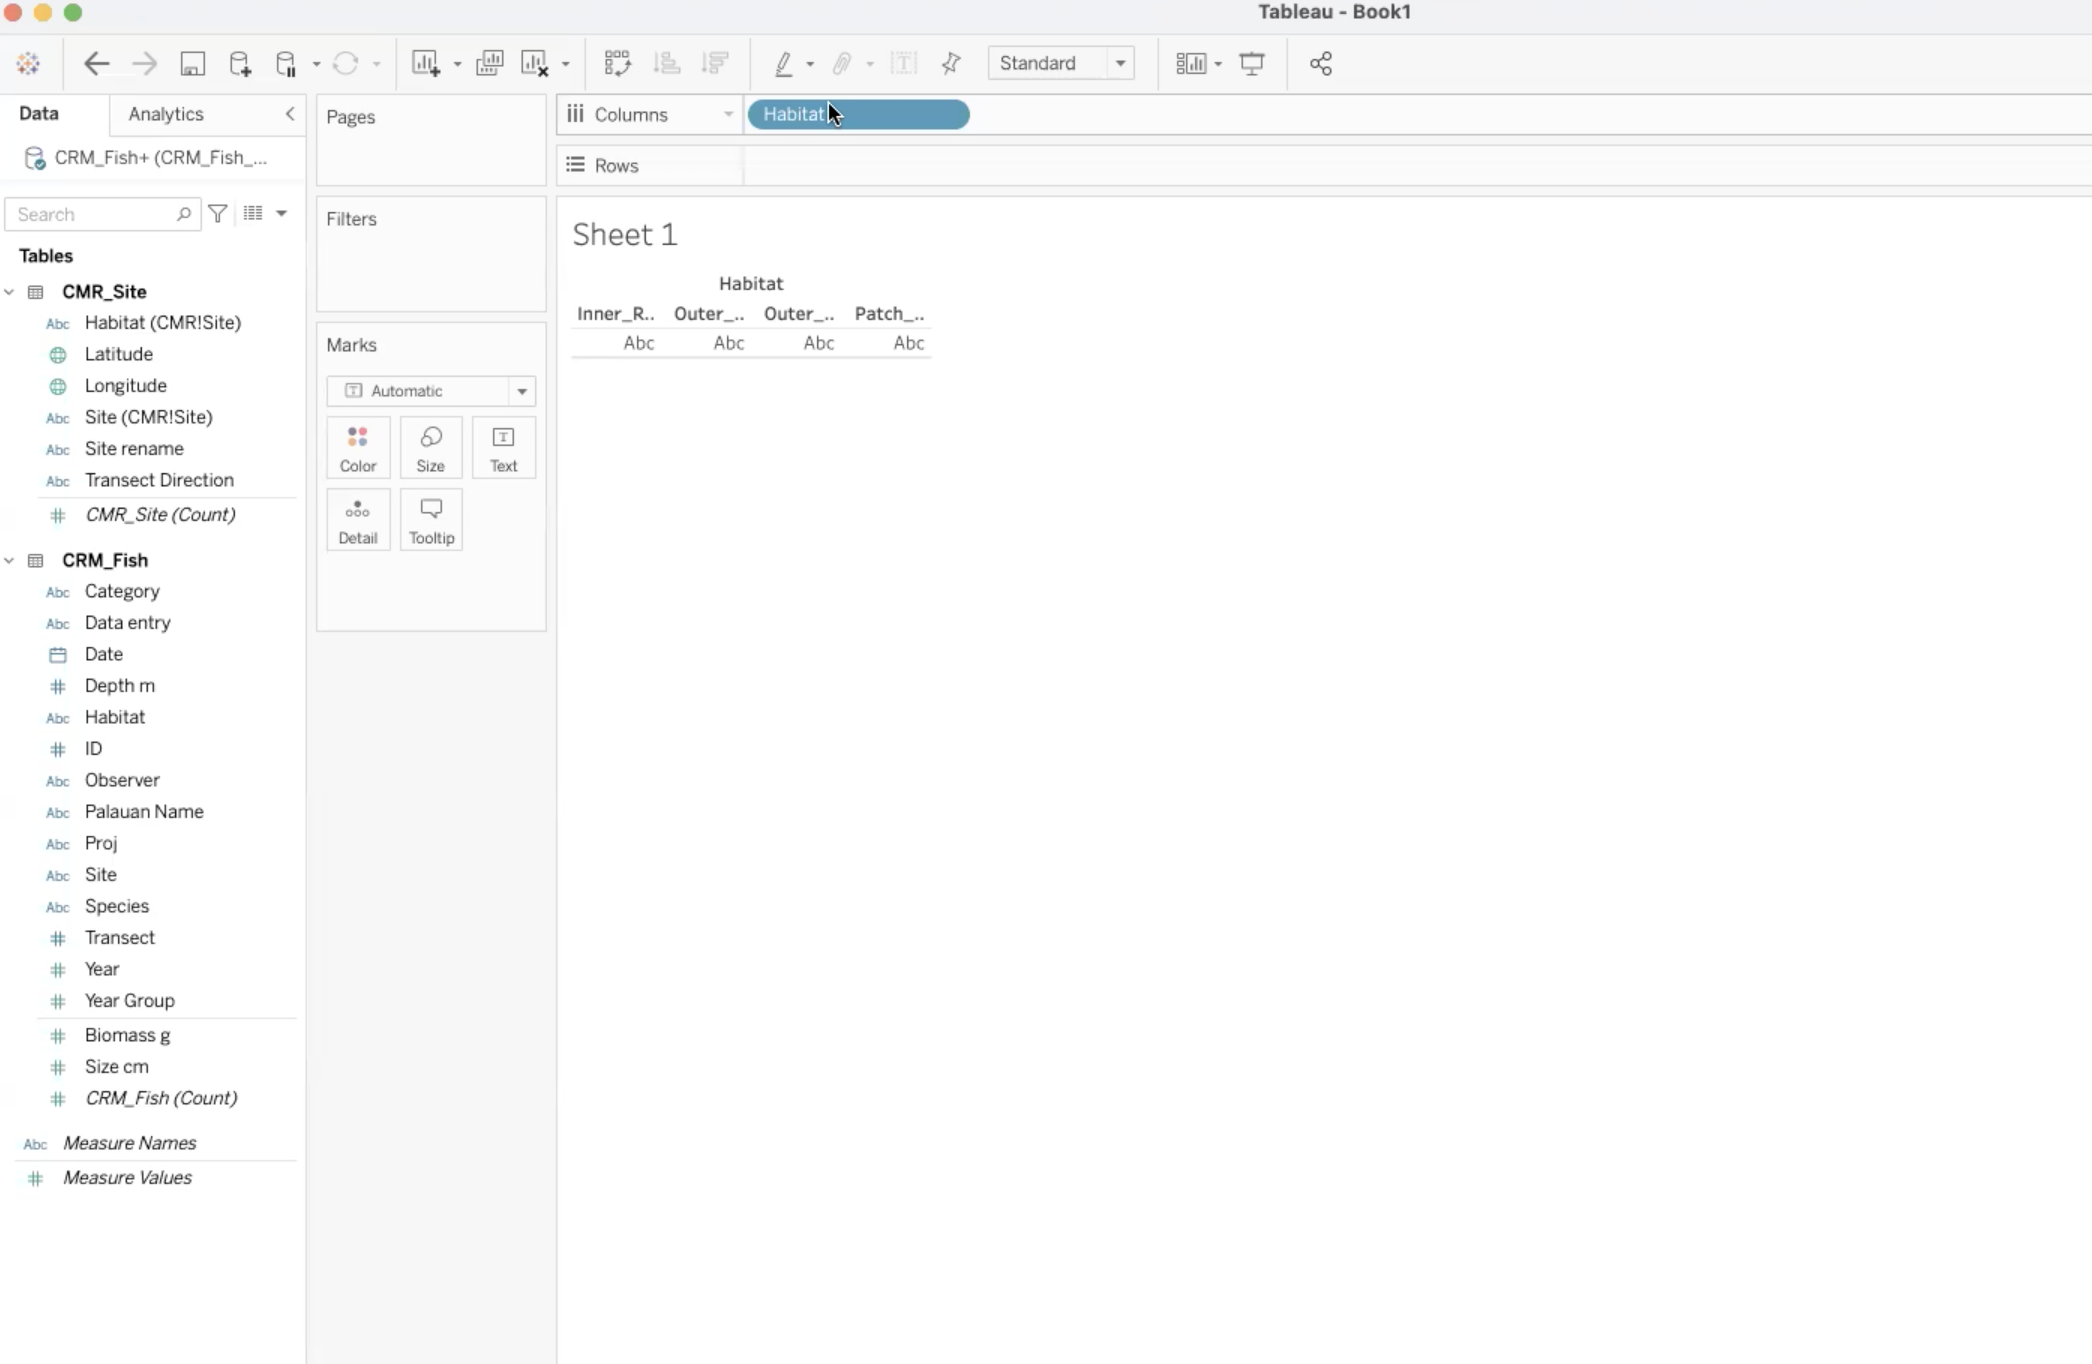
\includegraphics{images/M3S2_drag-habitat.png}

\begin{enumerate}
\def\labelenumi{\arabic{enumi}.}
\setcounter{enumi}{2}
\tightlist
\item
  Find \textbf{Biomass} under CRM\_Fish
\end{enumerate}

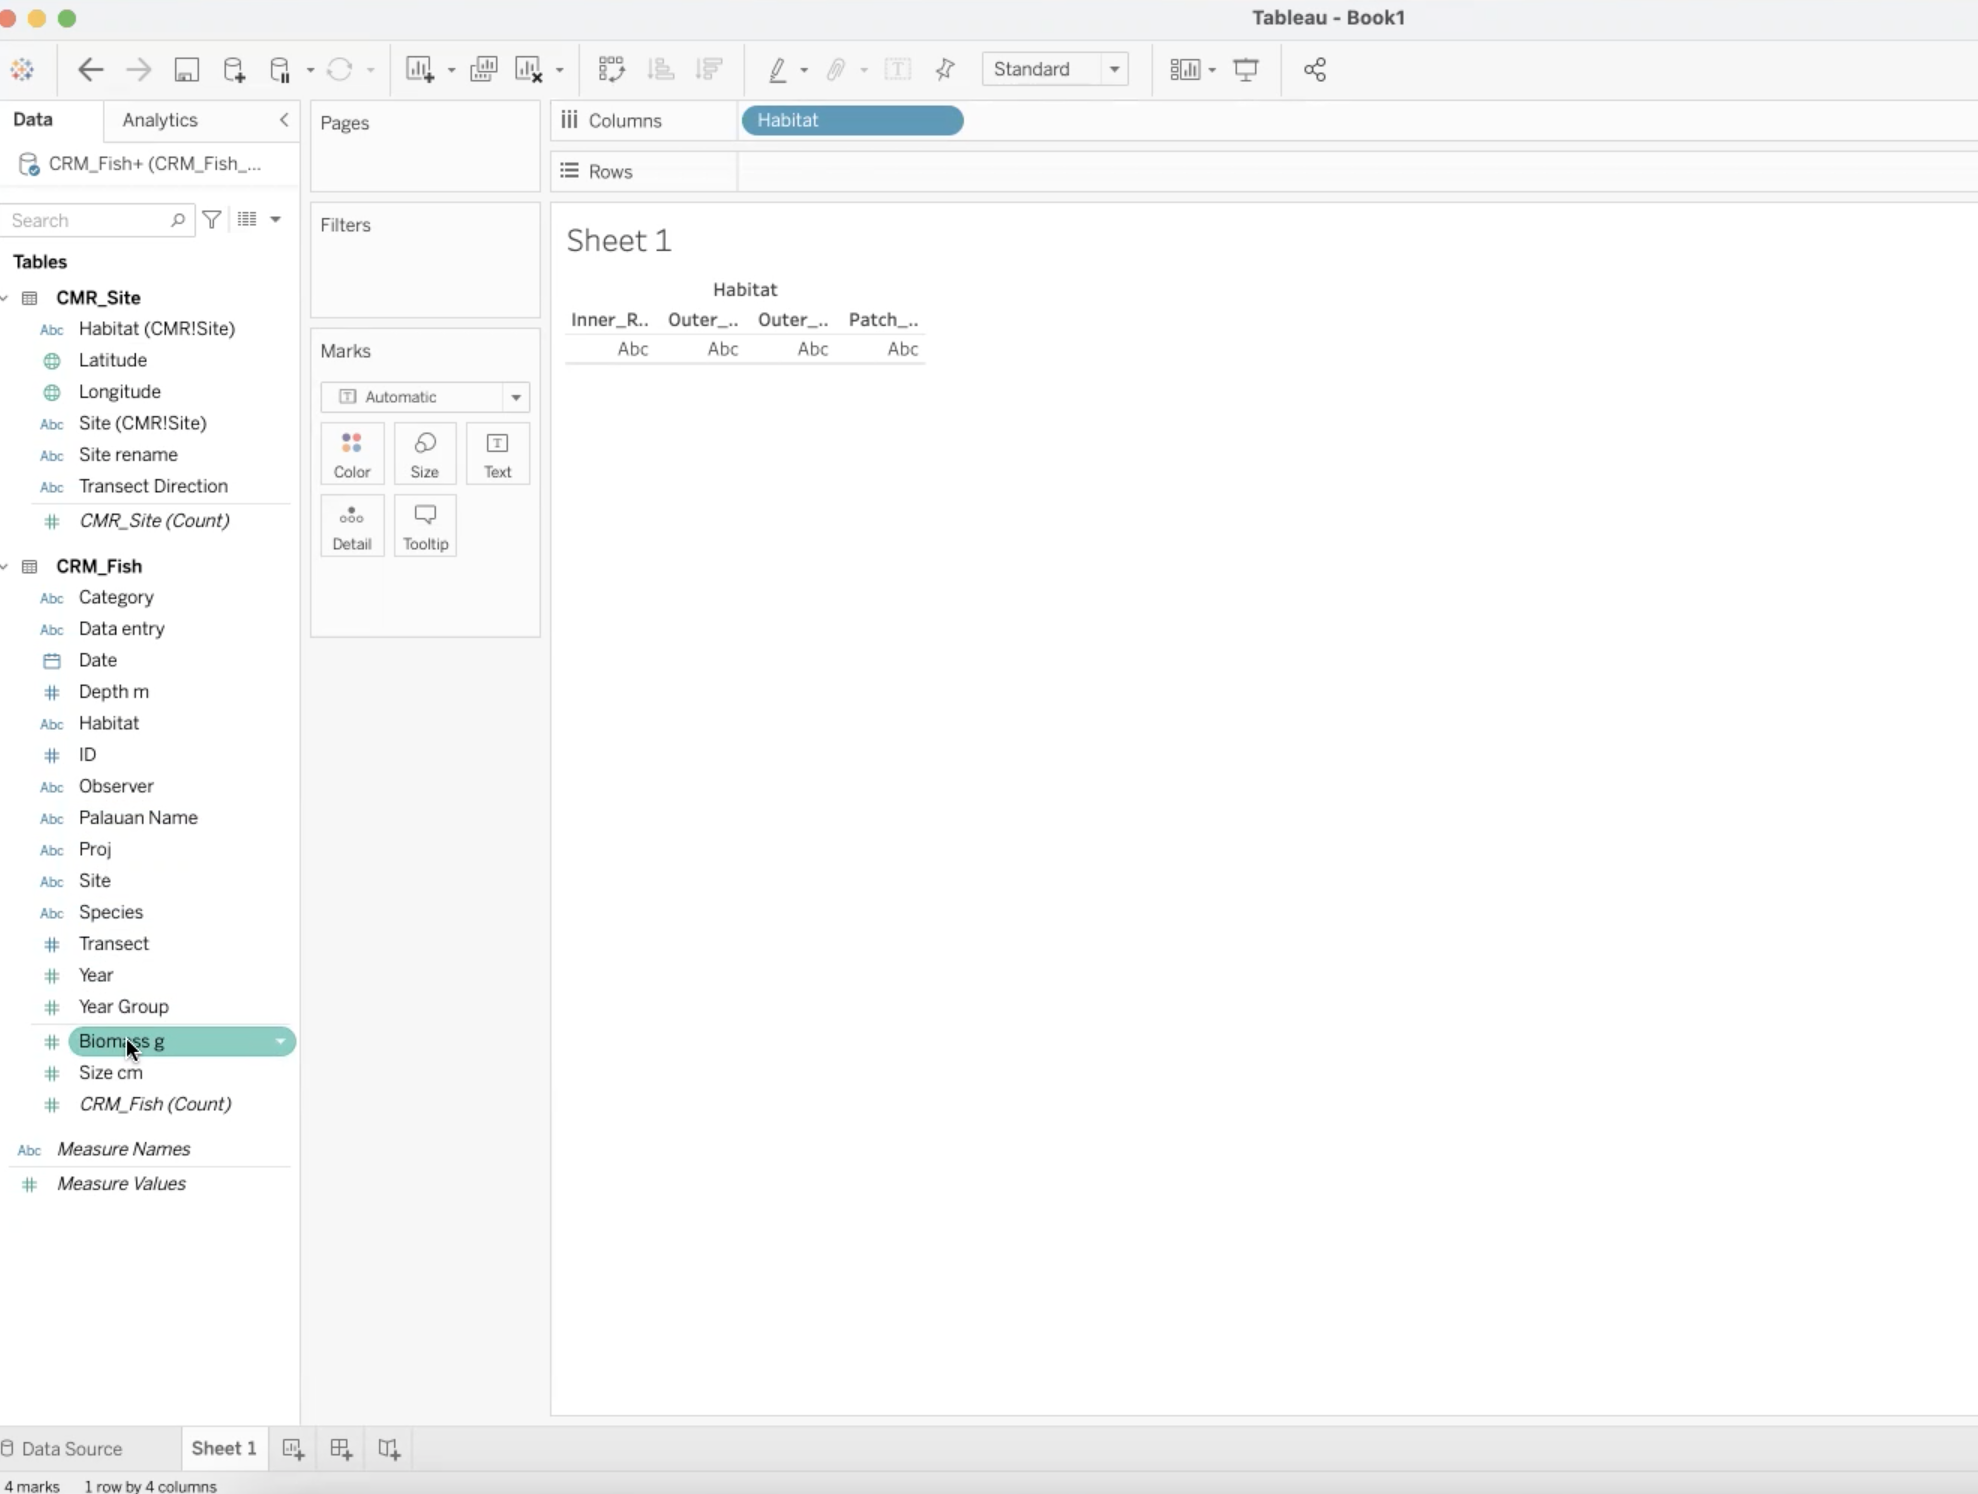
\includegraphics{images/M3S2_find-biomass.png}

\begin{enumerate}
\def\labelenumi{\arabic{enumi}.}
\setcounter{enumi}{3}
\tightlist
\item
  Drag and drop \textbf{Biomass} into \textbf{Rows}

  \begin{itemize}
  \tightlist
  \item
    This will place \textbf{Biomass} in the y-axis.
  \end{itemize}
\end{enumerate}

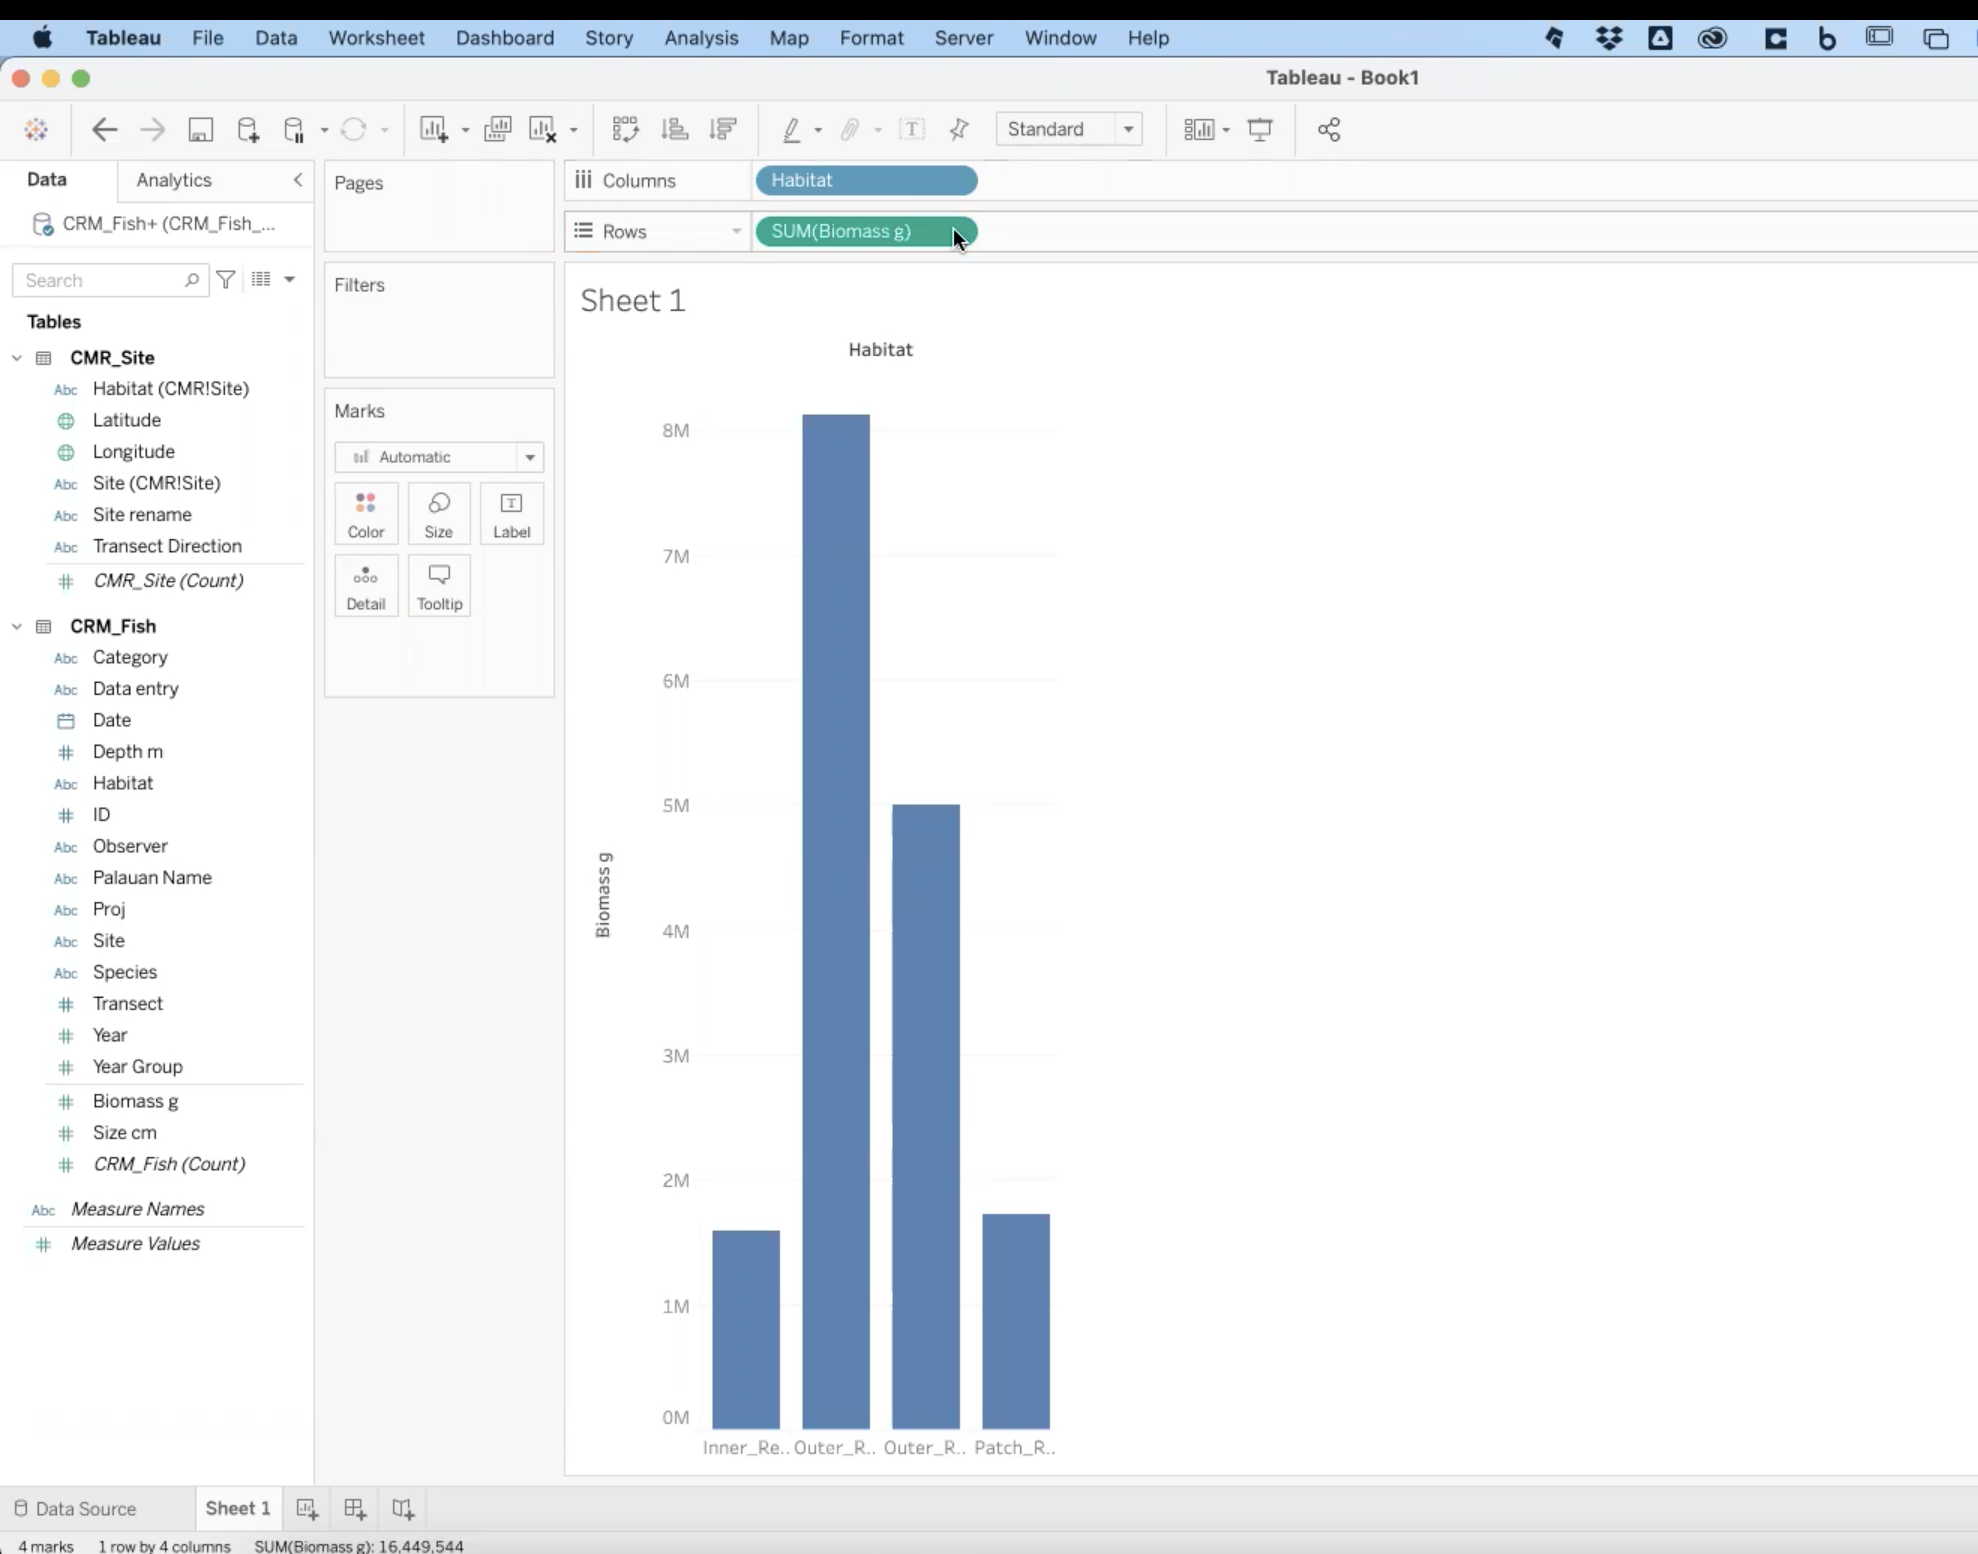
\includegraphics{images/M3S2_drag-biomass.png}

\begin{enumerate}
\def\labelenumi{\arabic{enumi}.}
\setcounter{enumi}{4}
\tightlist
\item
  Congratulations! You just made your first bar plot in Tableau!
\end{enumerate}

\textbf{\emph{Entire View and Sorting }}

\textbf{\emph{Show Me Menu}}

\begin{enumerate}
\def\labelenumi{\arabic{enumi}.}
\tightlist
\item
  The Show Me menu may pop up when you create a new graph. It looks like the image below.
\end{enumerate}

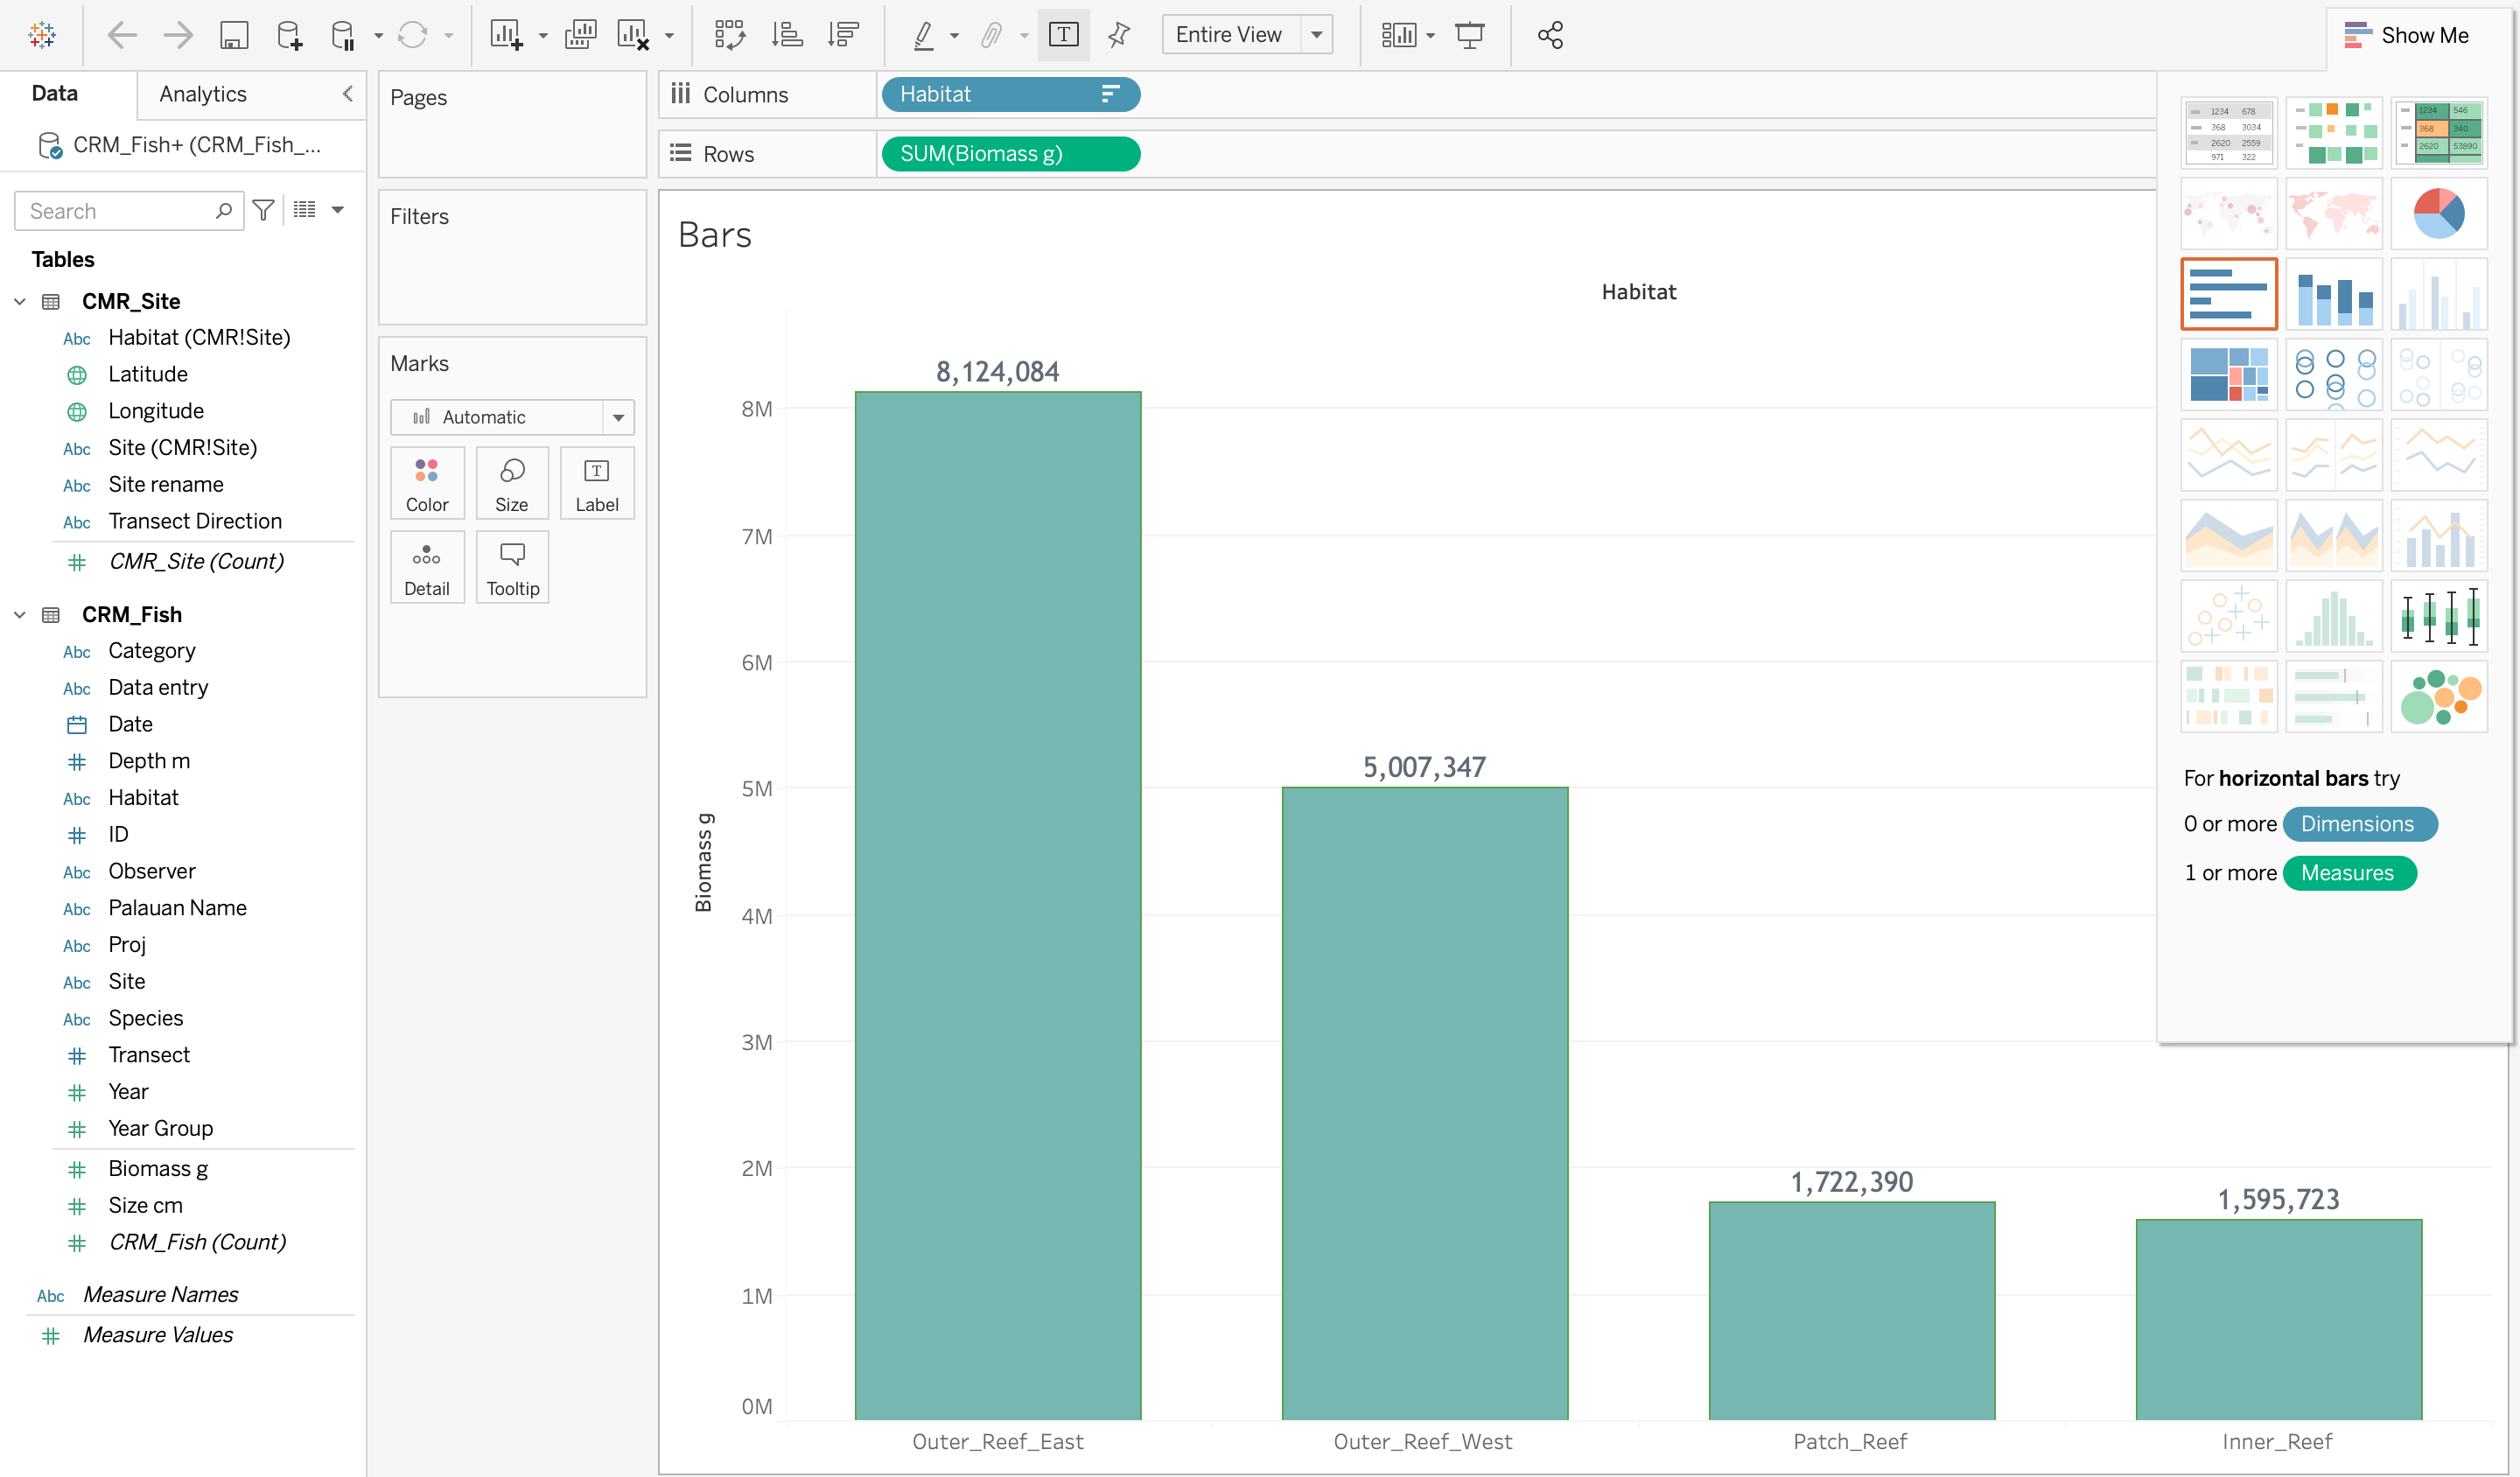
\includegraphics{images/M3S2_show-me-menu-full.png}

\begin{enumerate}
\def\labelenumi{\arabic{enumi}.}
\setcounter{enumi}{1}
\tightlist
\item
  If the Show Me menu obscures your view, you can simply click on \textbf{Show Me} at the top and the menu will collapse.
\end{enumerate}

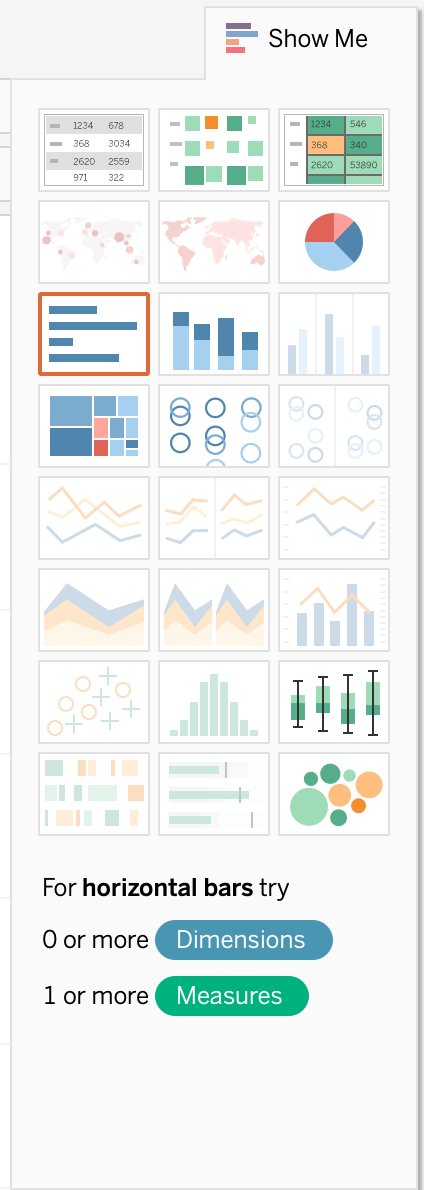
\includegraphics{images/M3S2_show-me-menu-zoom.png}

\begin{enumerate}
\def\labelenumi{\arabic{enumi}.}
\setcounter{enumi}{2}
\tightlist
\item
  How to use the \textbf{Show Me} menu
\end{enumerate}

\textbf{\emph{Troubleshooting: Switching Rows and Columns}}

\begin{enumerate}
\def\labelenumi{\arabic{enumi}.}
\tightlist
\item
  Lilli has a question that came up when she was exploring the Show Me menu. When she tried to go back to a bar chart, the chart was flipped! Watch Alfredo's answer:
\end{enumerate}

\hypertarget{basic-plots-using-the-marks-menu}{%
\subsection{Basic plots using the Marks menu}\label{basic-plots-using-the-marks-menu}}

\begin{enumerate}
\def\labelenumi{\arabic{enumi}.}
\tightlist
\item
  The Show Me menu is a great tool where Tableau can suggest automated graphs, but we want to teach you how to take full control of Tableau. In order to do that, we will utilize the Marks menu.

  \begin{itemize}
  \tightlist
  \item
    The Marks menu is located to the left of your bar graph:
  \end{itemize}
\end{enumerate}

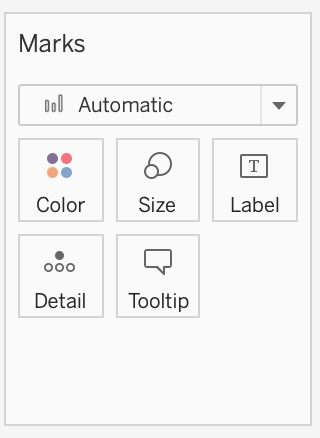
\includegraphics{images/M3S2_Marks-Menu.png}

\begin{enumerate}
\def\labelenumi{\arabic{enumi}.}
\setcounter{enumi}{1}
\item
  Color

  \begin{itemize}
  \item
    Here you can customize the color, opacity, and border of your graph.
    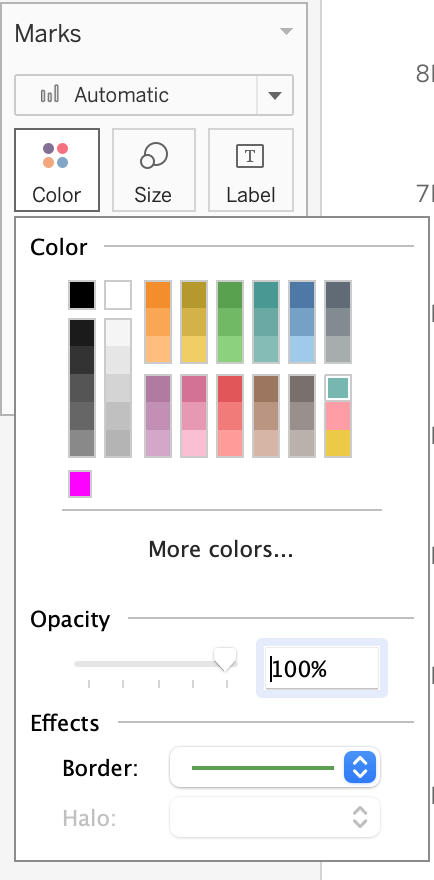
\includegraphics{images/M3S2_color-marks-menu.png}
  \item
    Click on \textbf{More colors\ldots{}} and you will see even more options to customize your color palette.
  \item
    Practice: Insert a Hex Color

    \begin{itemize}
    \tightlist
    \item
      Find the Hex Color field under \textbf{More colors\ldots{}}

      \begin{itemize}
      \tightlist
      \item
        For example, here is the ``RGB Sliders'' window on a Mac.
        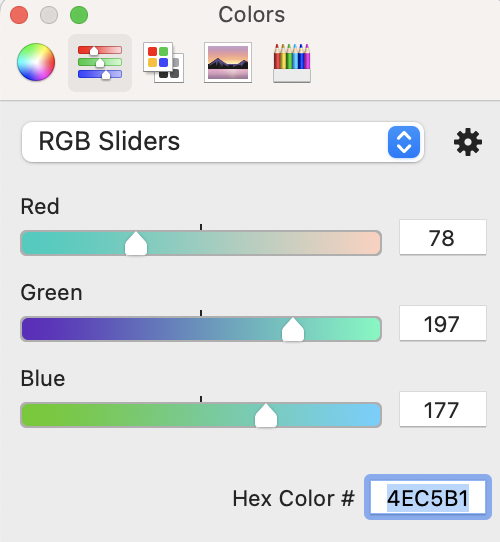
\includegraphics{images/M3S2_RGB-Sliders-Marks-Menu.png}
      \item
        Type or paste \textbf{4EC5B1} in the Hex Color \#
      \item
        Now, your graph should be this color:
        
\includegraphics{images/M3S2_Hex-Code-Medium-Turquoise.png}
      \end{itemize}
    \end{itemize}
  \end{itemize}
\item
  Size

  \begin{itemize}
  \tightlist
  \item
    If you click on Size, a slider will appear. In bar graphs, the slider changes the width of each bar. Let's see how Size affects a pie chart.

    \begin{itemize}
    \tightlist
    \item
      First, name this sheet ``Bars.'' {REMEMBER TO ALWAYS NAME YOUR SHEETS}\\
    \end{itemize}
  \item
    To edit, double-click on the bottom where it says ``Sheet 1''
    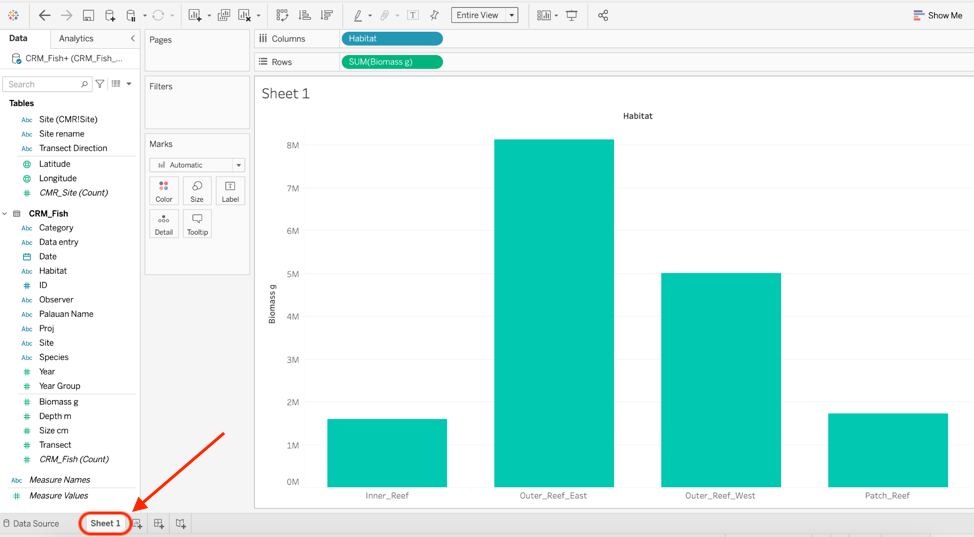
\includegraphics{images/M3S2_rename-sheets.png}
  \item
    Create a new worksheet by clicking on the button directly to the right of ``Bars''.
    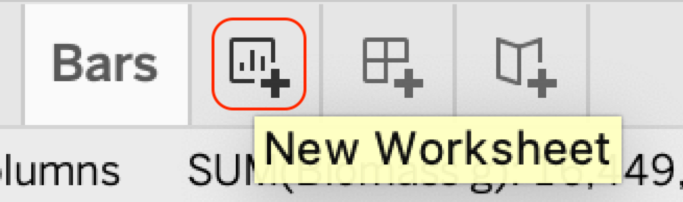
\includegraphics{images/M3S2_button.png}
  \item
    Name this sheet ``Pie''.
  \item
    In the new sheet, create exactly the same graph. Drag \textbf{Habitat} into \textbf{Columns} and \textbf{Biomass} into \textbf{Rows}.
  \item
    Go to \textbf{Show Me} and choose Pie Chart.

    \begin{itemize}
    \tightlist
    \item
      The pie chart will look very small, so change the view to Entire View. Your current sheet should look like the image below:
      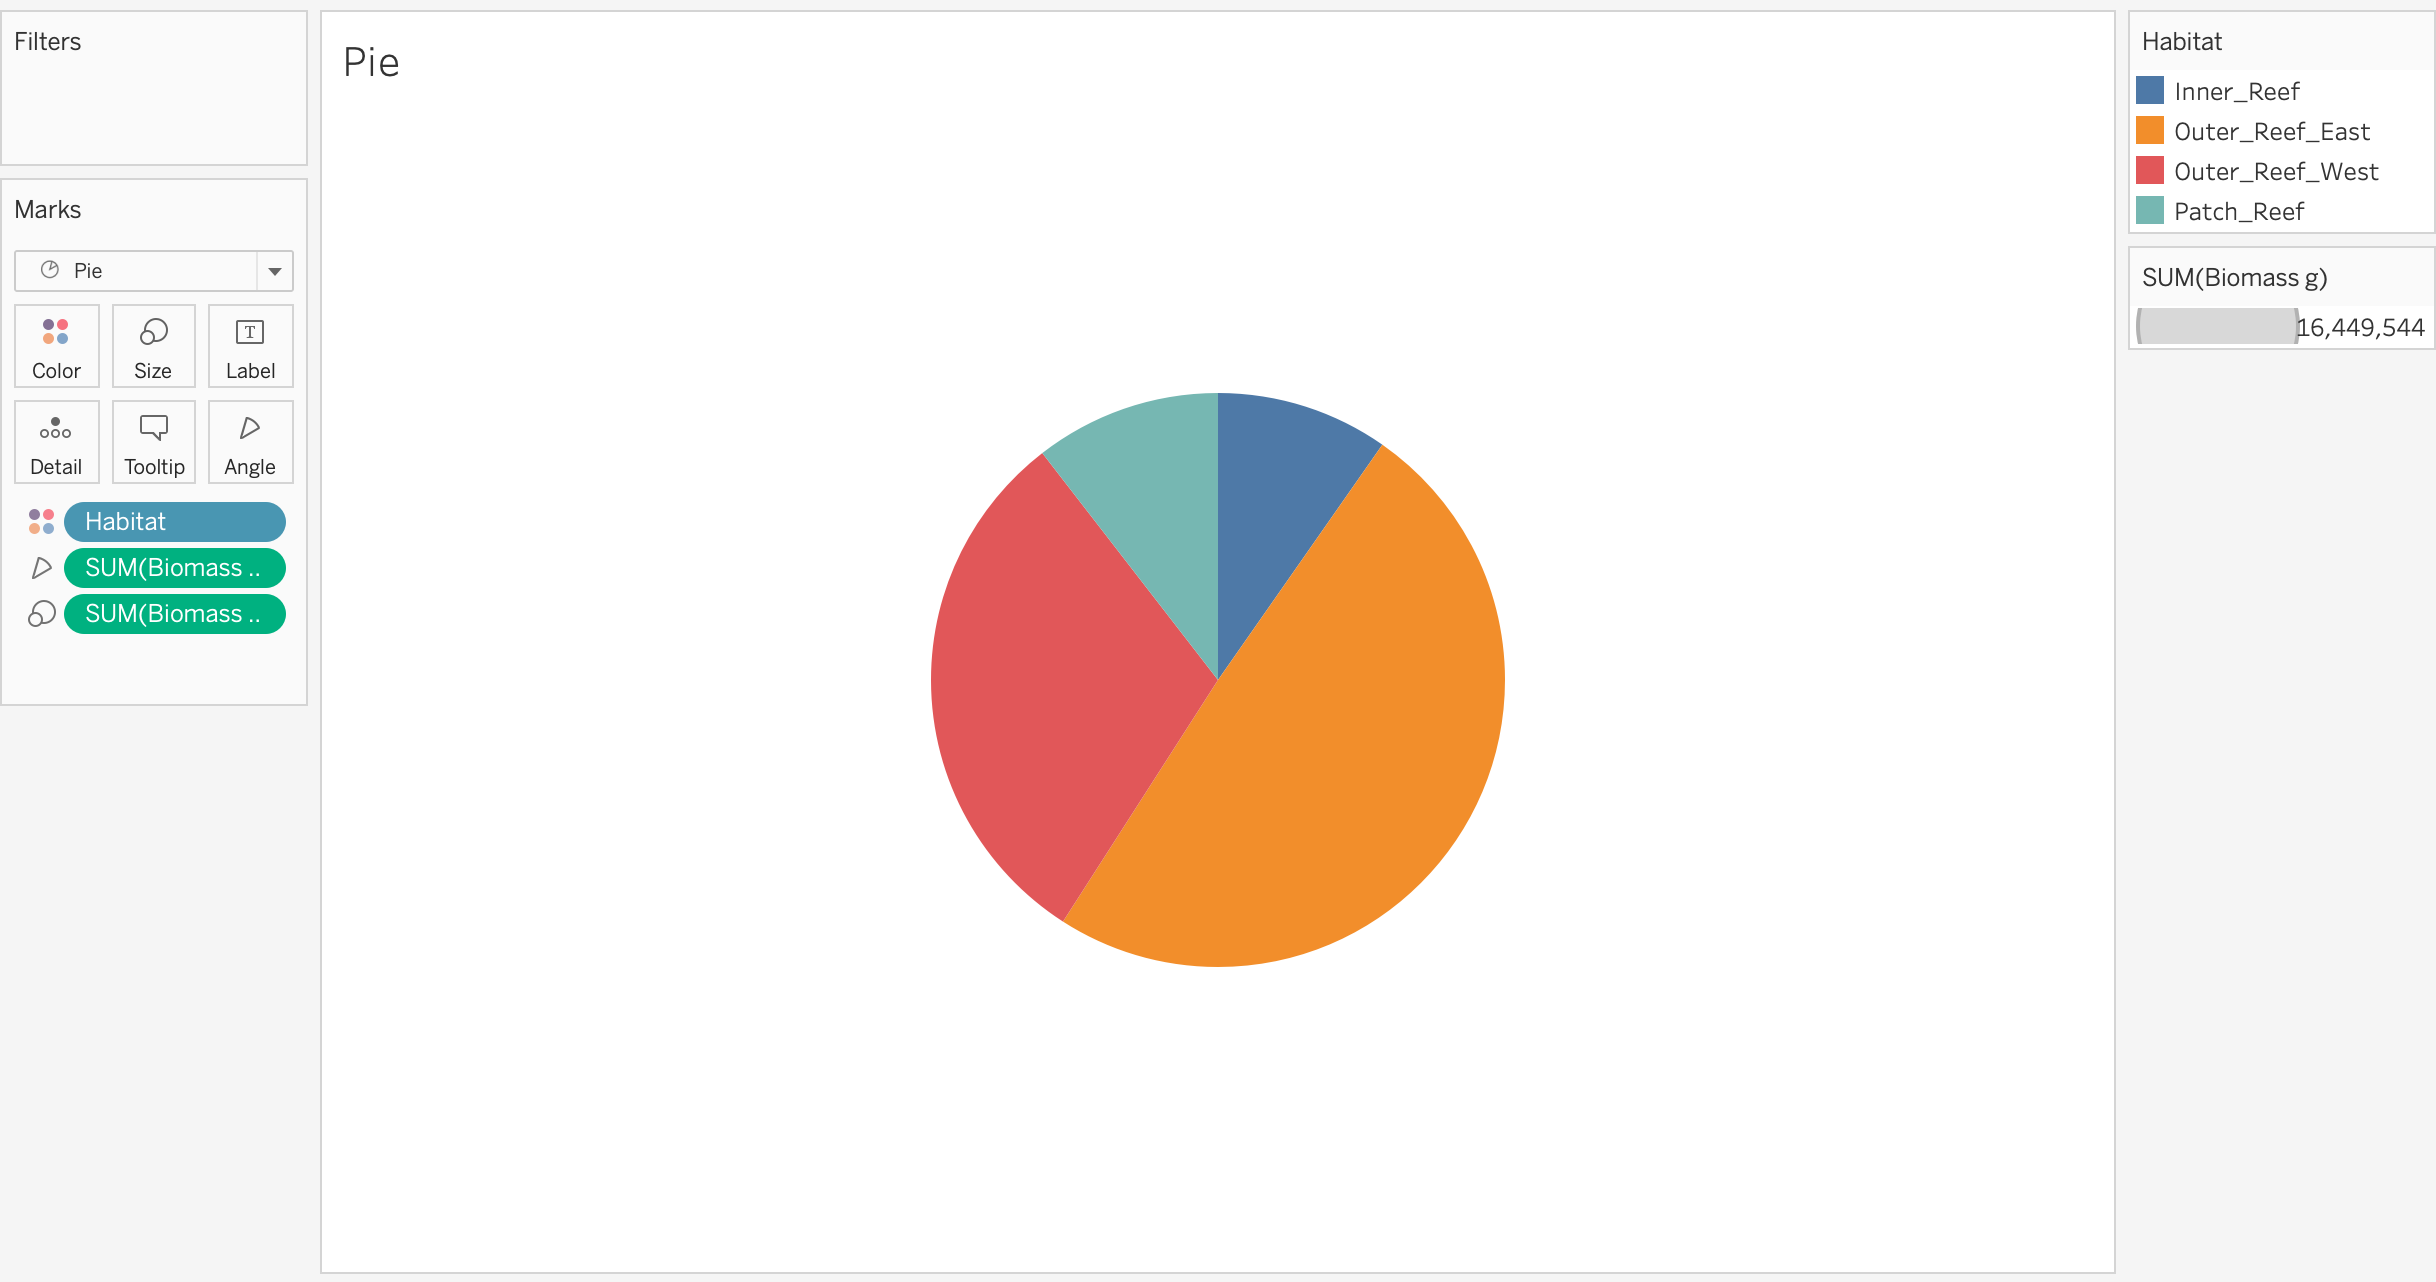
\includegraphics{images/M3S2_Pie-Chart.png}
    \end{itemize}
  \item
    Try using the \textbf{Size} function in the \textbf{Marks} menu. Notice that when you change the size of this graph, you are changing the size of the whole pie chart.
  \end{itemize}
\end{enumerate}

\begin{itemize}
\tightlist
\item
  When you are changing something like the size, you have to experiment a bit to see what the software will do. Each graph type will respond differently to changing the size.
\end{itemize}

\begin{enumerate}
\def\labelenumi{\arabic{enumi}.}
\setcounter{enumi}{3}
\tightlist
\item
  Labels
\end{enumerate}

\begin{enumerate}
\def\labelenumi{\arabic{enumi}.}
\setcounter{enumi}{4}
\item
  Details

  \begin{itemize}
  \tightlist
  \item
    We will cover the Details marks in a \protect\hyperlink{tableau-dashboards-part-1-basic-dashboards}{later session}.
  \end{itemize}
\item
  Tooltip
\end{enumerate}

\hypertarget{line-plot}{%
\subsection{Line Plot}\label{line-plot}}

\begin{enumerate}
\def\labelenumi{\arabic{enumi}.}
\item
  Practice Exercise: Create and modify a \textbf{Line Plot}

  \begin{itemize}
  \tightlist
  \item
    Create a new sheet and name it ``Line''.
  \item
    Drag \textbf{Year} into \textbf{Columns} and drag \textbf{Size} into \textbf{Rows}.
  \item
    For a line plot, summing the size of all the fish doesn't make much sense. In this case, showing the average size of the fish per year makes more sense, so let's do that.
  \item
    Right click on the field where it says \textbf{SUM (Size cm)} and a drop down menu will appear. Choose \textbf{Measure}, then click on \textbf{Average}.
  \end{itemize}

  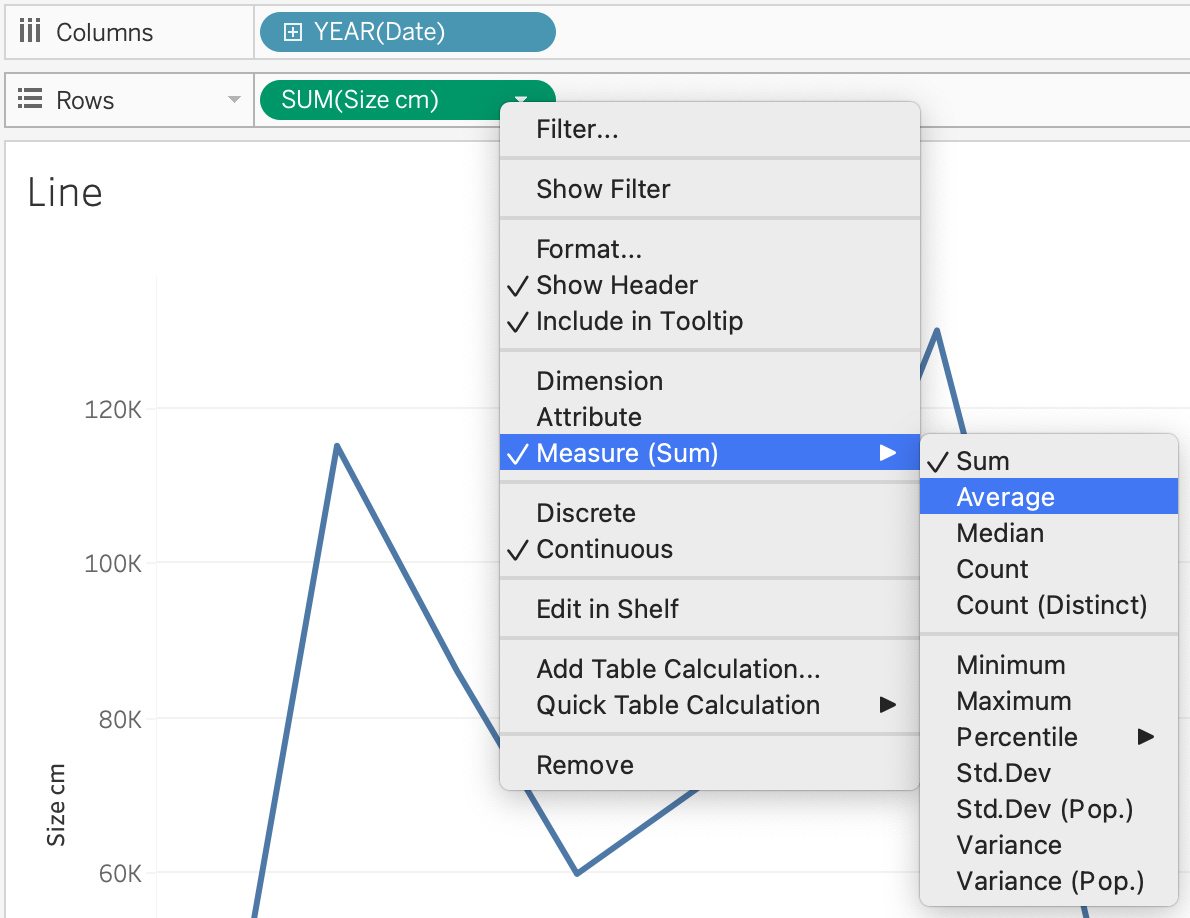
\includegraphics{images/M3S2_change-measure.png}

  \begin{itemize}
  \tightlist
  \item
    Does your plot now look like the image below? If so, you can move on to the next steps.
  \end{itemize}
\end{enumerate}

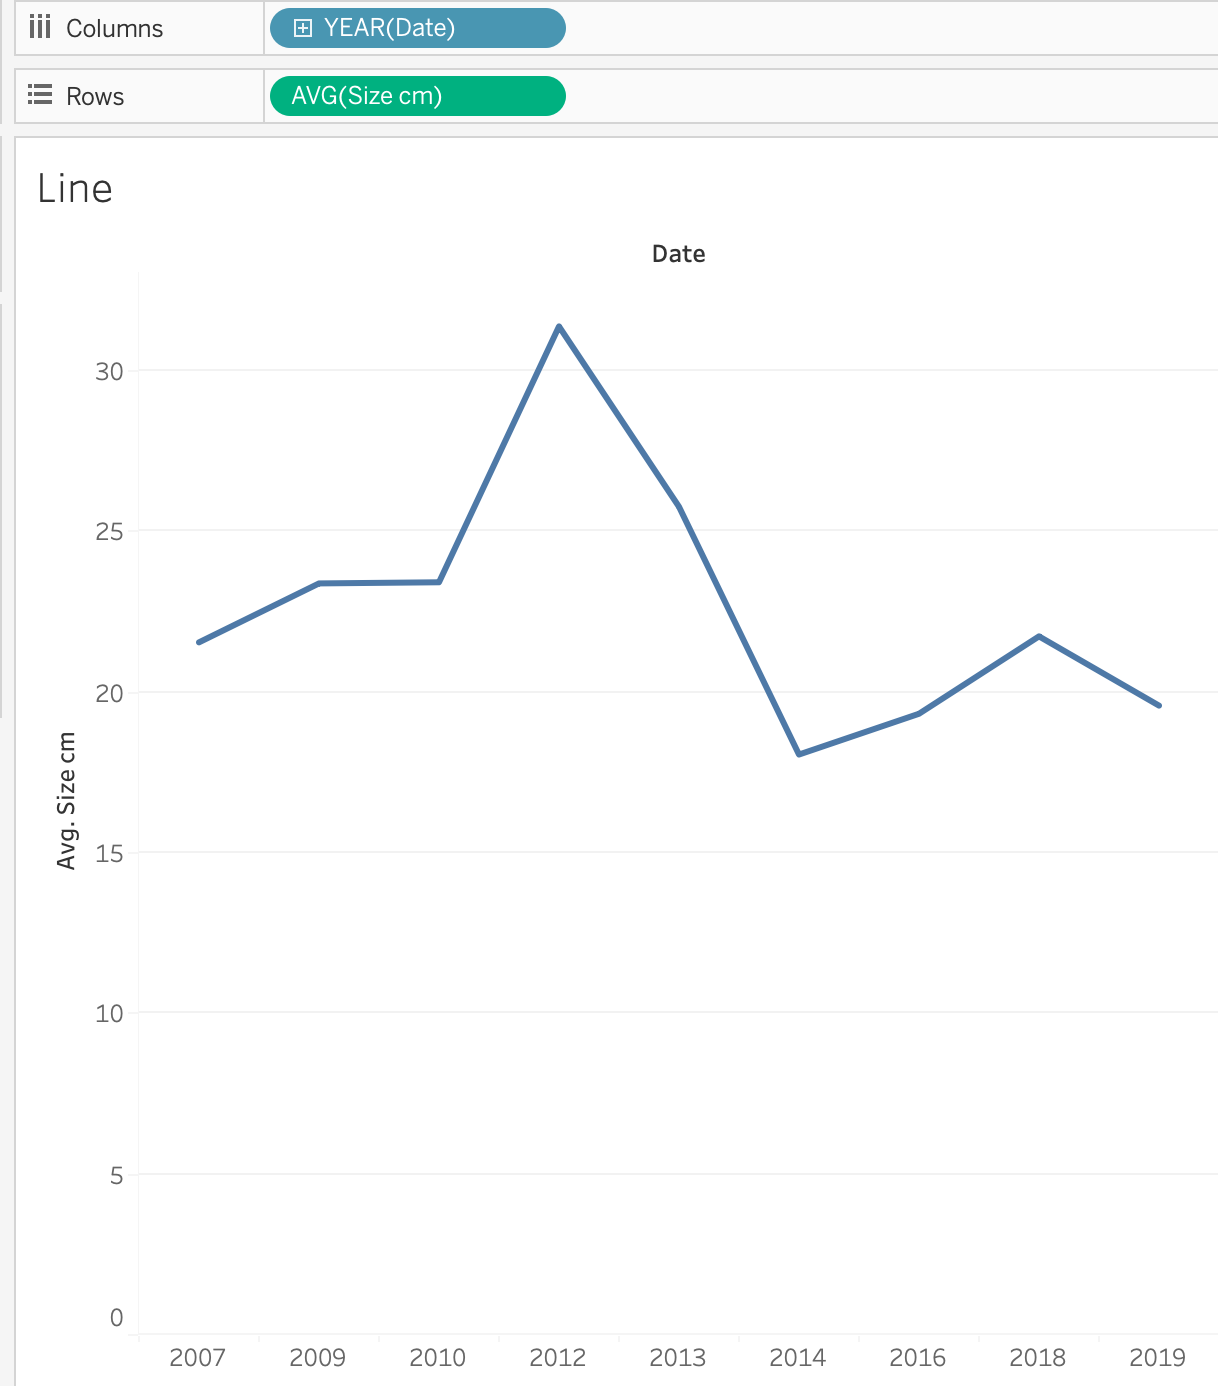
\includegraphics{images/M3S2_Line-Plot.png}

\hypertarget{area-plot}{%
\subsection{Area plot}\label{area-plot}}

\begin{enumerate}
\def\labelenumi{\arabic{enumi}.}
\tightlist
\item
  Good job! From here, it is easy to change your \textbf{Line} plot to an \textbf{Area} plot. Under the \textbf{Marks} menu, open the dropdown menu where it says \textbf{Automatic} and click on \textbf{Area}.
\end{enumerate}

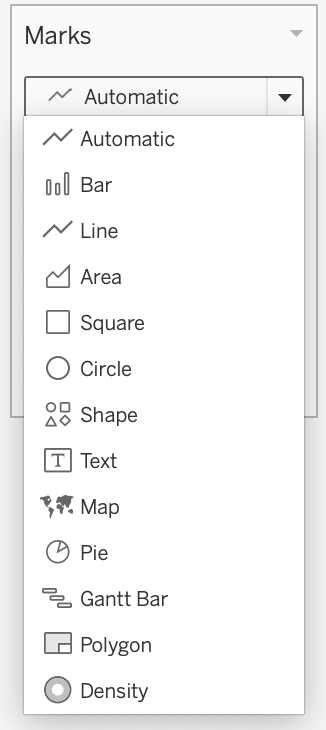
\includegraphics{images/M3S2_Plot-types.png}

\begin{enumerate}
\def\labelenumi{\arabic{enumi}.}
\setcounter{enumi}{1}
\tightlist
\item
  As you can see, there are many options in this dropdown menu. This is where you can manually change the type of plot displayed.
\end{enumerate}

\hypertarget{map}{%
\subsection{Map}\label{map}}

\begin{enumerate}
\def\labelenumi{\arabic{enumi}.}
\tightlist
\item
  There are two ways to create a map.
\item
  First, on a new sheet you can drag and drop \textbf{Longitude} to \textbf{Columns} and \textbf{Latitude} to \textbf{Rows}.

  \begin{itemize}
  \tightlist
  \item
    \emph{Remember that Columns are the x-axis and Rows are the y-axis.}\\
  \item
    Your map should look like this:
    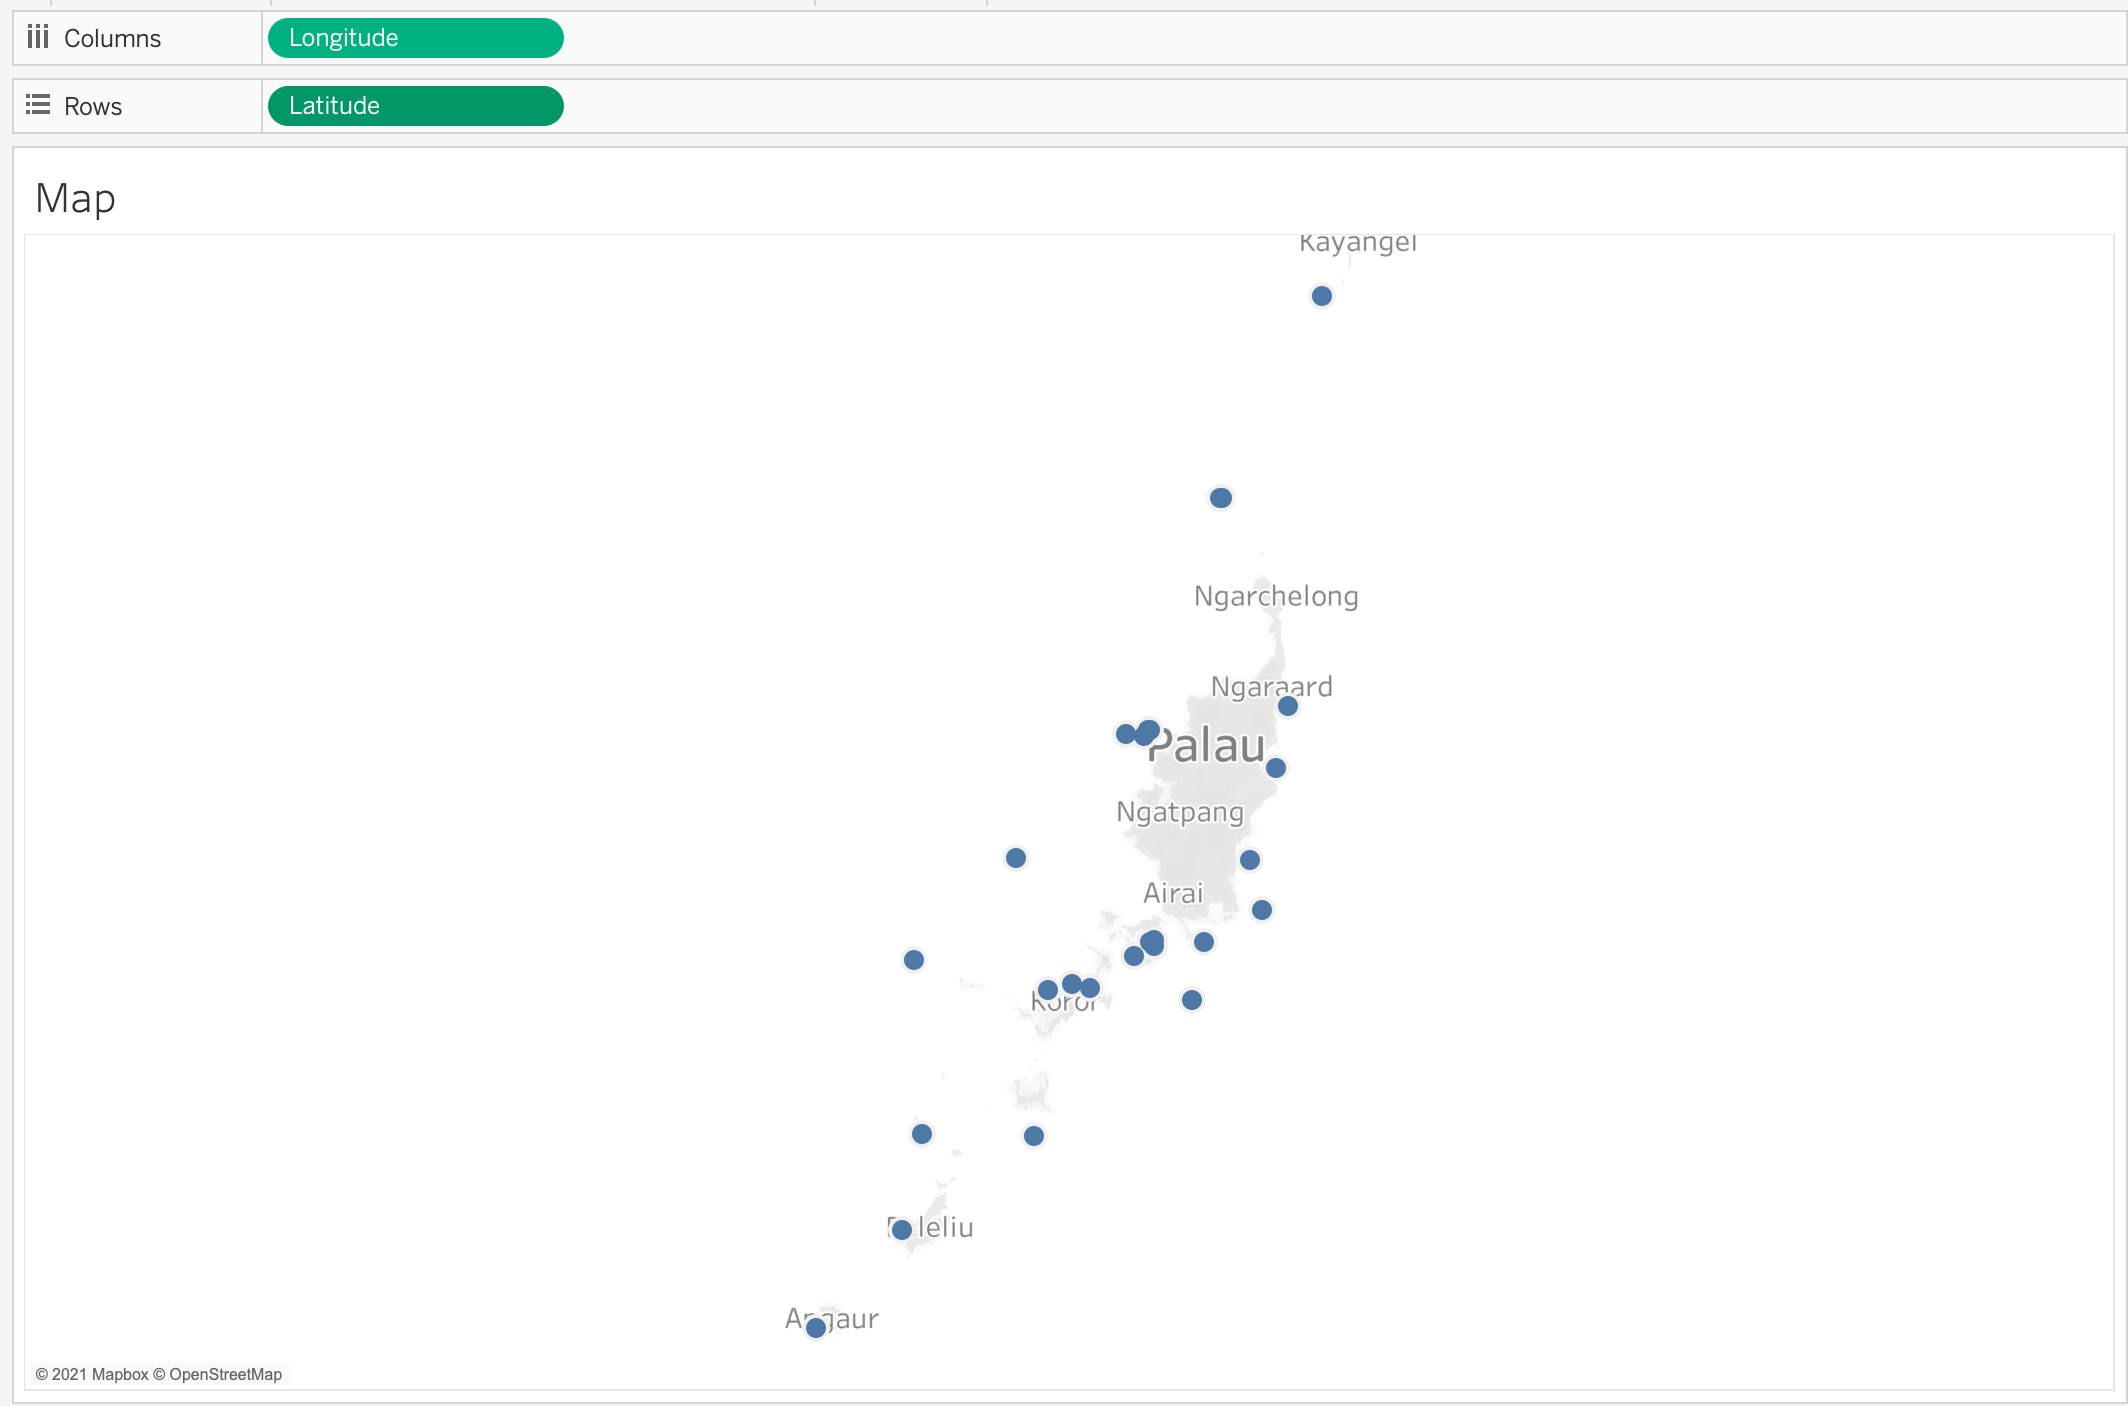
\includegraphics{images/M3S2_map-1.png}
  \end{itemize}
\item
  Next, clear the \textbf{Columns} and \textbf{Rows} fields. You can do this either by right-clicking and then choosing \textbf{Remove} or you can drag \textbf{Longitude} and \textbf{Latitude} back into the left column.
\end{enumerate}

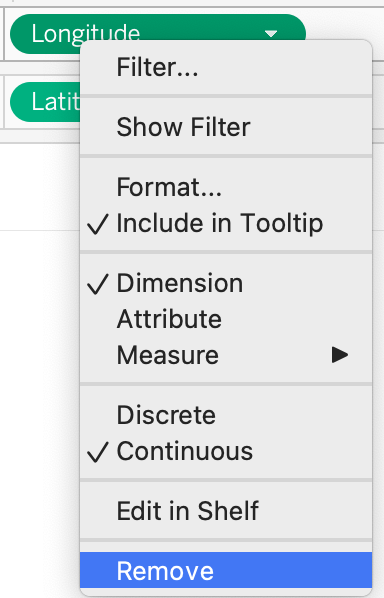
\includegraphics{images/M3S2_remove-column.png}

\begin{enumerate}
\def\labelenumi{\arabic{enumi}.}
\setcounter{enumi}{3}
\tightlist
\item
  Second, there is an even easier way to plug in geographic spatial data. Double-click \textbf{Latitude} and then double-click \textbf{Longitude}. If you assigned the data properly (i.e.~Dimension, Geographic Role: Latitude), Tableau will know exactly how to create this map for you.

  \begin{itemize}
  \tightlist
  \item
    Your map should look exactly the same as the previous visualization:
    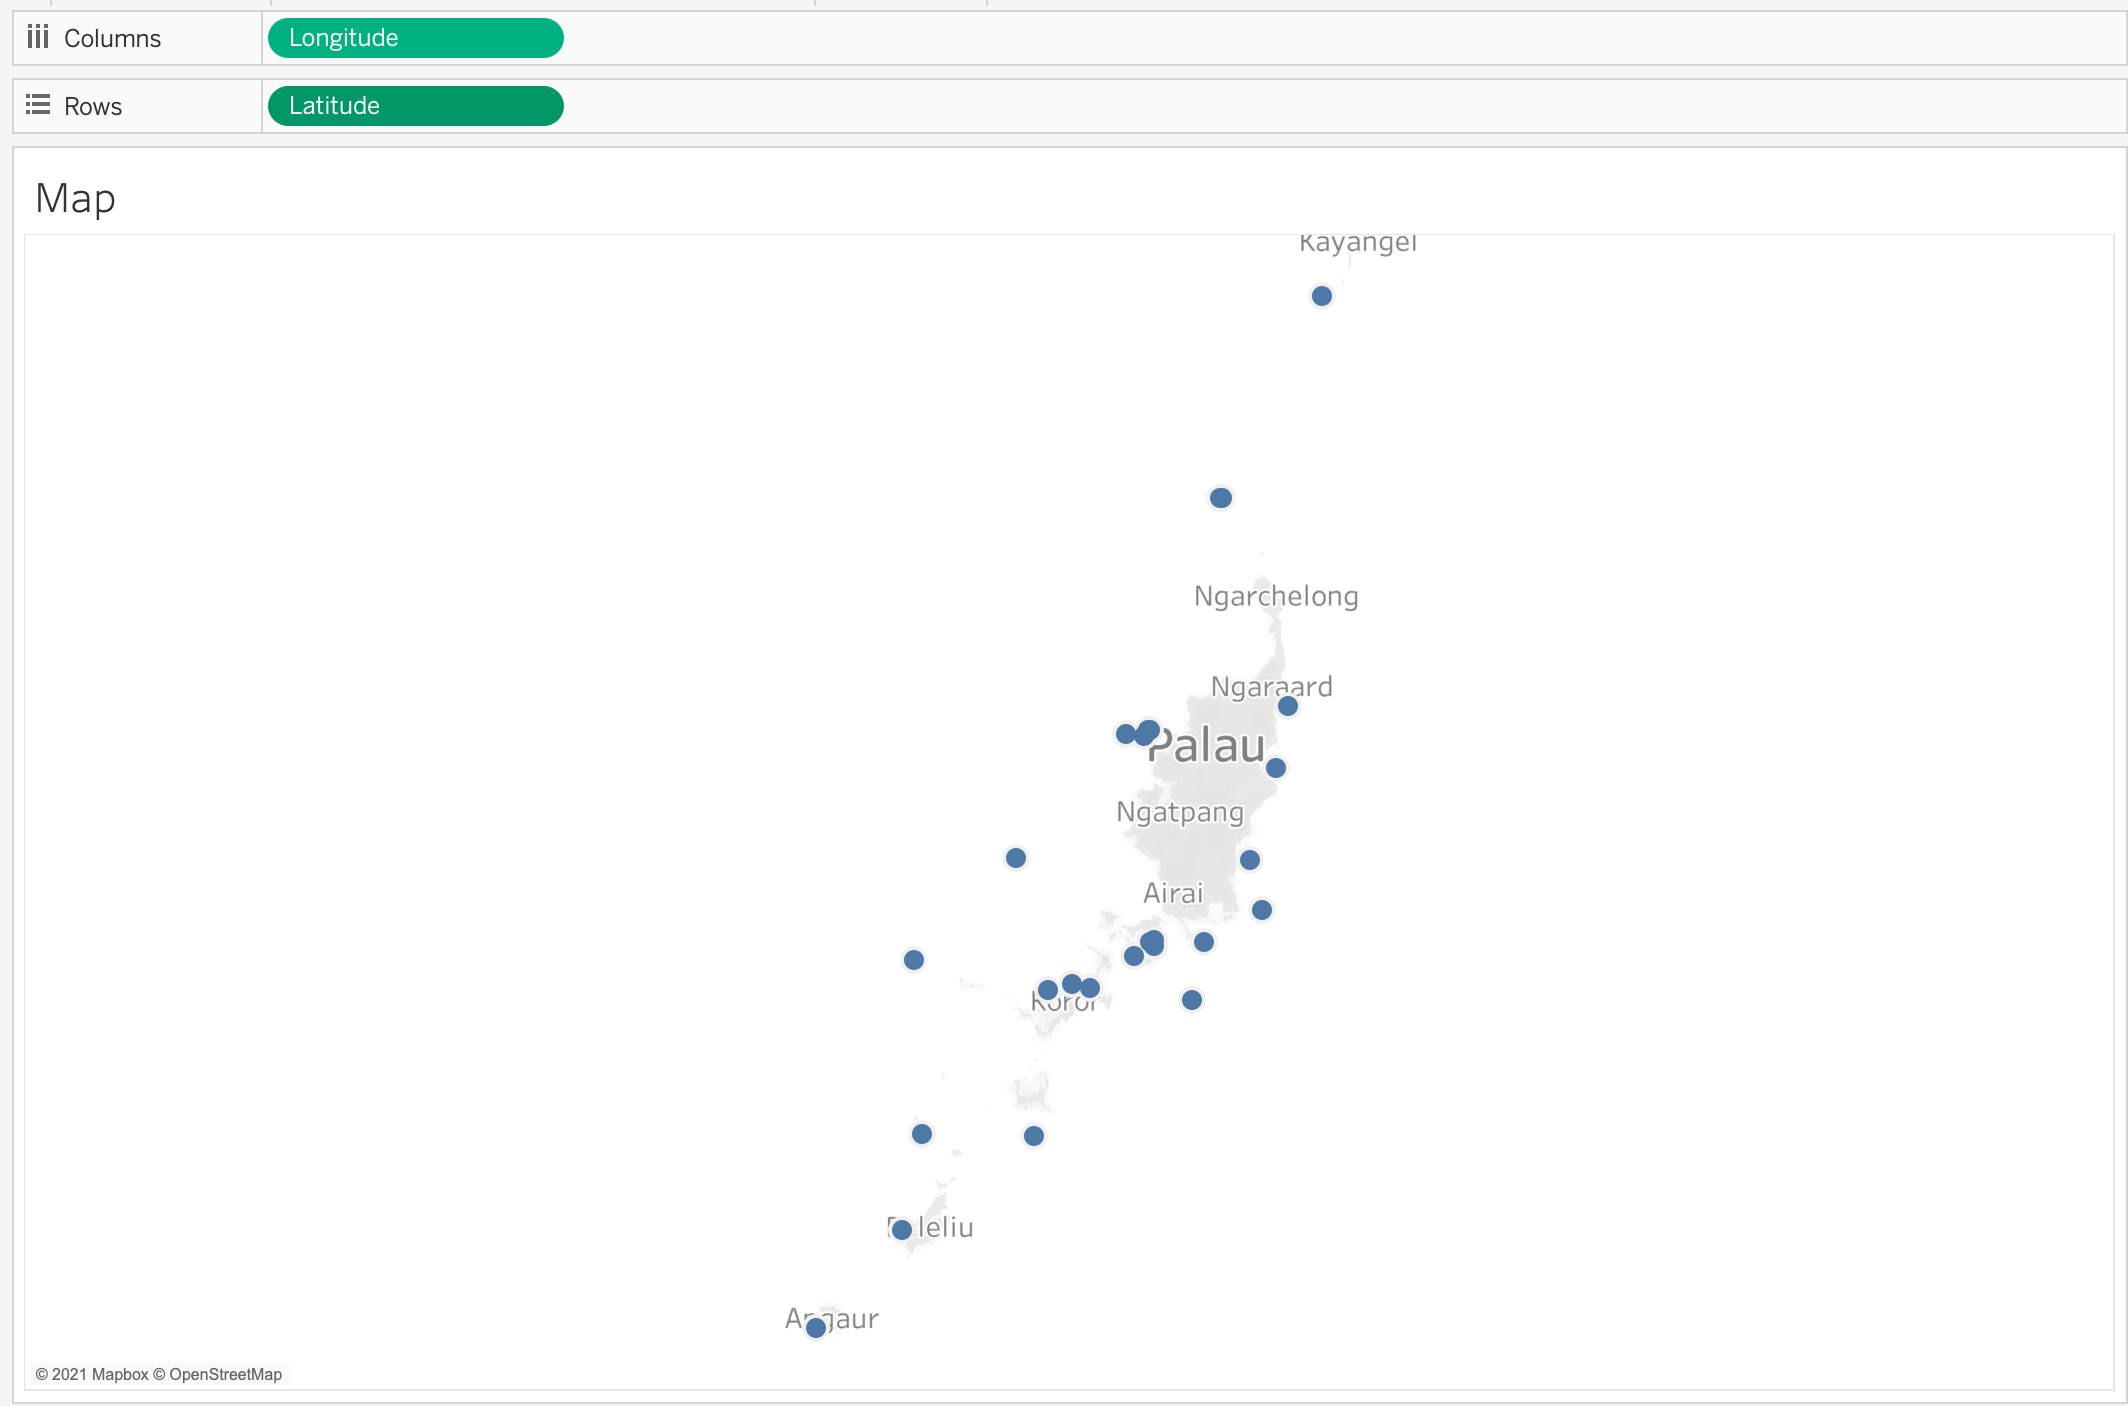
\includegraphics{images/M3S2_map-1.png}
  \end{itemize}
\item
  Name this sheet ``Map''
\item
  Customizing the Map using the \textbf{Marks} menu

  \begin{itemize}
  \tightlist
  \item
    Using the \textbf{Color} tool, change the color of the elements to a preferred color and add a black border.
  \item
    Using the \textbf{Size} tool, make the elements a bit larger so you can see them better.

    \begin{itemize}
    \tightlist
    \item
      Remember that sliding to the right makes the elements larger and to the left makes them smaller.
    \end{itemize}
  \item
    Do you notice anything missing? If we were to show this map to a collaborator, they would only see the Longitude and Latitude, but not the Site name. Let's add the \textbf{Site} name to the \textbf{Tooltip} as dynamic text (or text that will be updated as the user interacts with the visualization).

    \begin{itemize}
    \tightlist
    \item
      Find \textbf{Site} in the left column under CRM\_Fish. Drag and drop \textbf{Site} into \textbf{Tooltip} in the Marks menu.
    \end{itemize}
  \item
    Edit \textbf{Tooltip} to clarify the map for users.

    \begin{itemize}
    \tightlist
    \item
      Click on \textbf{Tooltip} so we can edit the text. We want the name of the site to be at the top, so cut and paste ``Site: \textless ATTR(Site)\textgreater{}'' to move it above Latitude and Longitude.
    \item
      Delete the static text ``Site:'' leaving just ``\textless ATTR(Site)\textgreater{}'' at the top.
    \item
      Select all the text and change the alignment to center.
    \item
      Next, add ``˚N'' to the right of \textless Latitude\textgreater{} and ``˚W'' to the right of \textless Longitude\textgreater{}

      \begin{itemize}
      \tightlist
      \item
        Mac shortcut: ``Option + Shift + 8''
      \item
        Windows shortcut: ``''Alt + 0176'' (with Num Lock on)
      \item
        If you have trouble with the degree symbol, copy and paste from this text: ˚N ˚W
        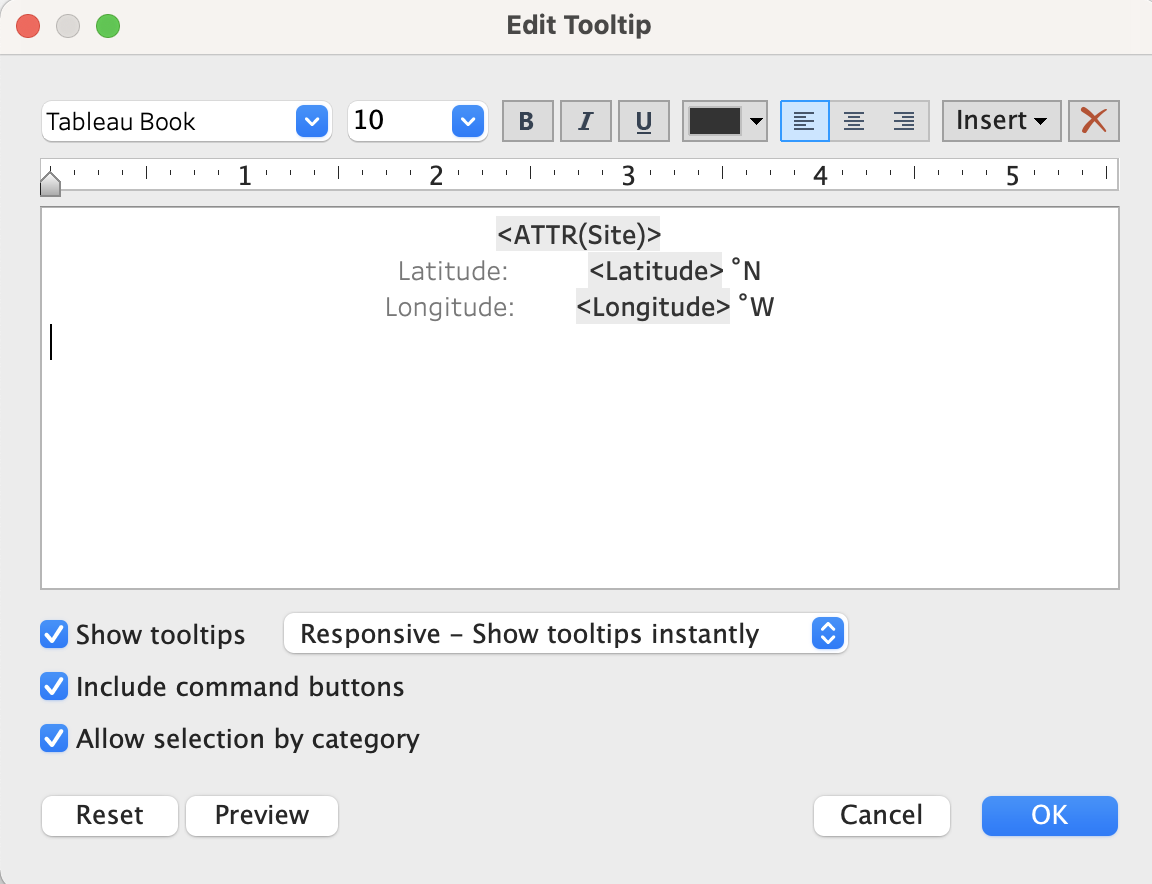
\includegraphics{images/M3S2_edit-tooltip-for-map.png}
      \end{itemize}
    \item
      Click \textbf{OK} to close the editing window and hover your cursor over your map to check that the tooltip is working.
      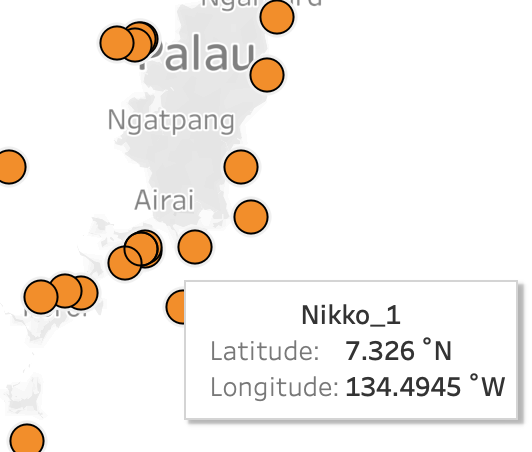
\includegraphics{images/M3S2_check-tooltip-for-map.png}
    \end{itemize}
  \end{itemize}
\item
  You have just created an interactive map showing the various sites around Palau where data was collected.

  \begin{itemize}
  \tightlist
  \item
    Take a moment to explore the functionality of the map you created by moving your cursor around the map and clicking on a few of the data points.
  \end{itemize}
\end{enumerate}

\hypertarget{bubble-plot}{%
\subsection{Bubble plot}\label{bubble-plot}}

\begin{enumerate}
\def\labelenumi{\arabic{enumi}.}
\tightlist
\item
  To create a Bubble plot, you always start with a Bar plot.

  \begin{itemize}
  \tightlist
  \item
    In a new sheet, drag and drop \textbf{Species} into \textbf{Columns} and \textbf{Biomass} into \textbf{Rows}.
  \item
    Then, click on \textbf{Show Me} and choose \textbf{Bubble}.
    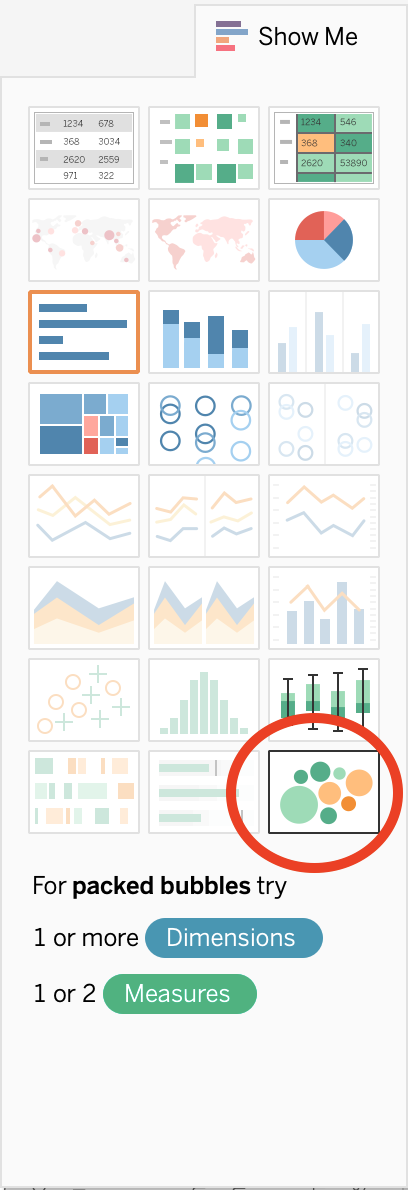
\includegraphics{images/M3S2_show-me-bubble-plot.png}
  \item
    E Voilá! A Bubble plot!
    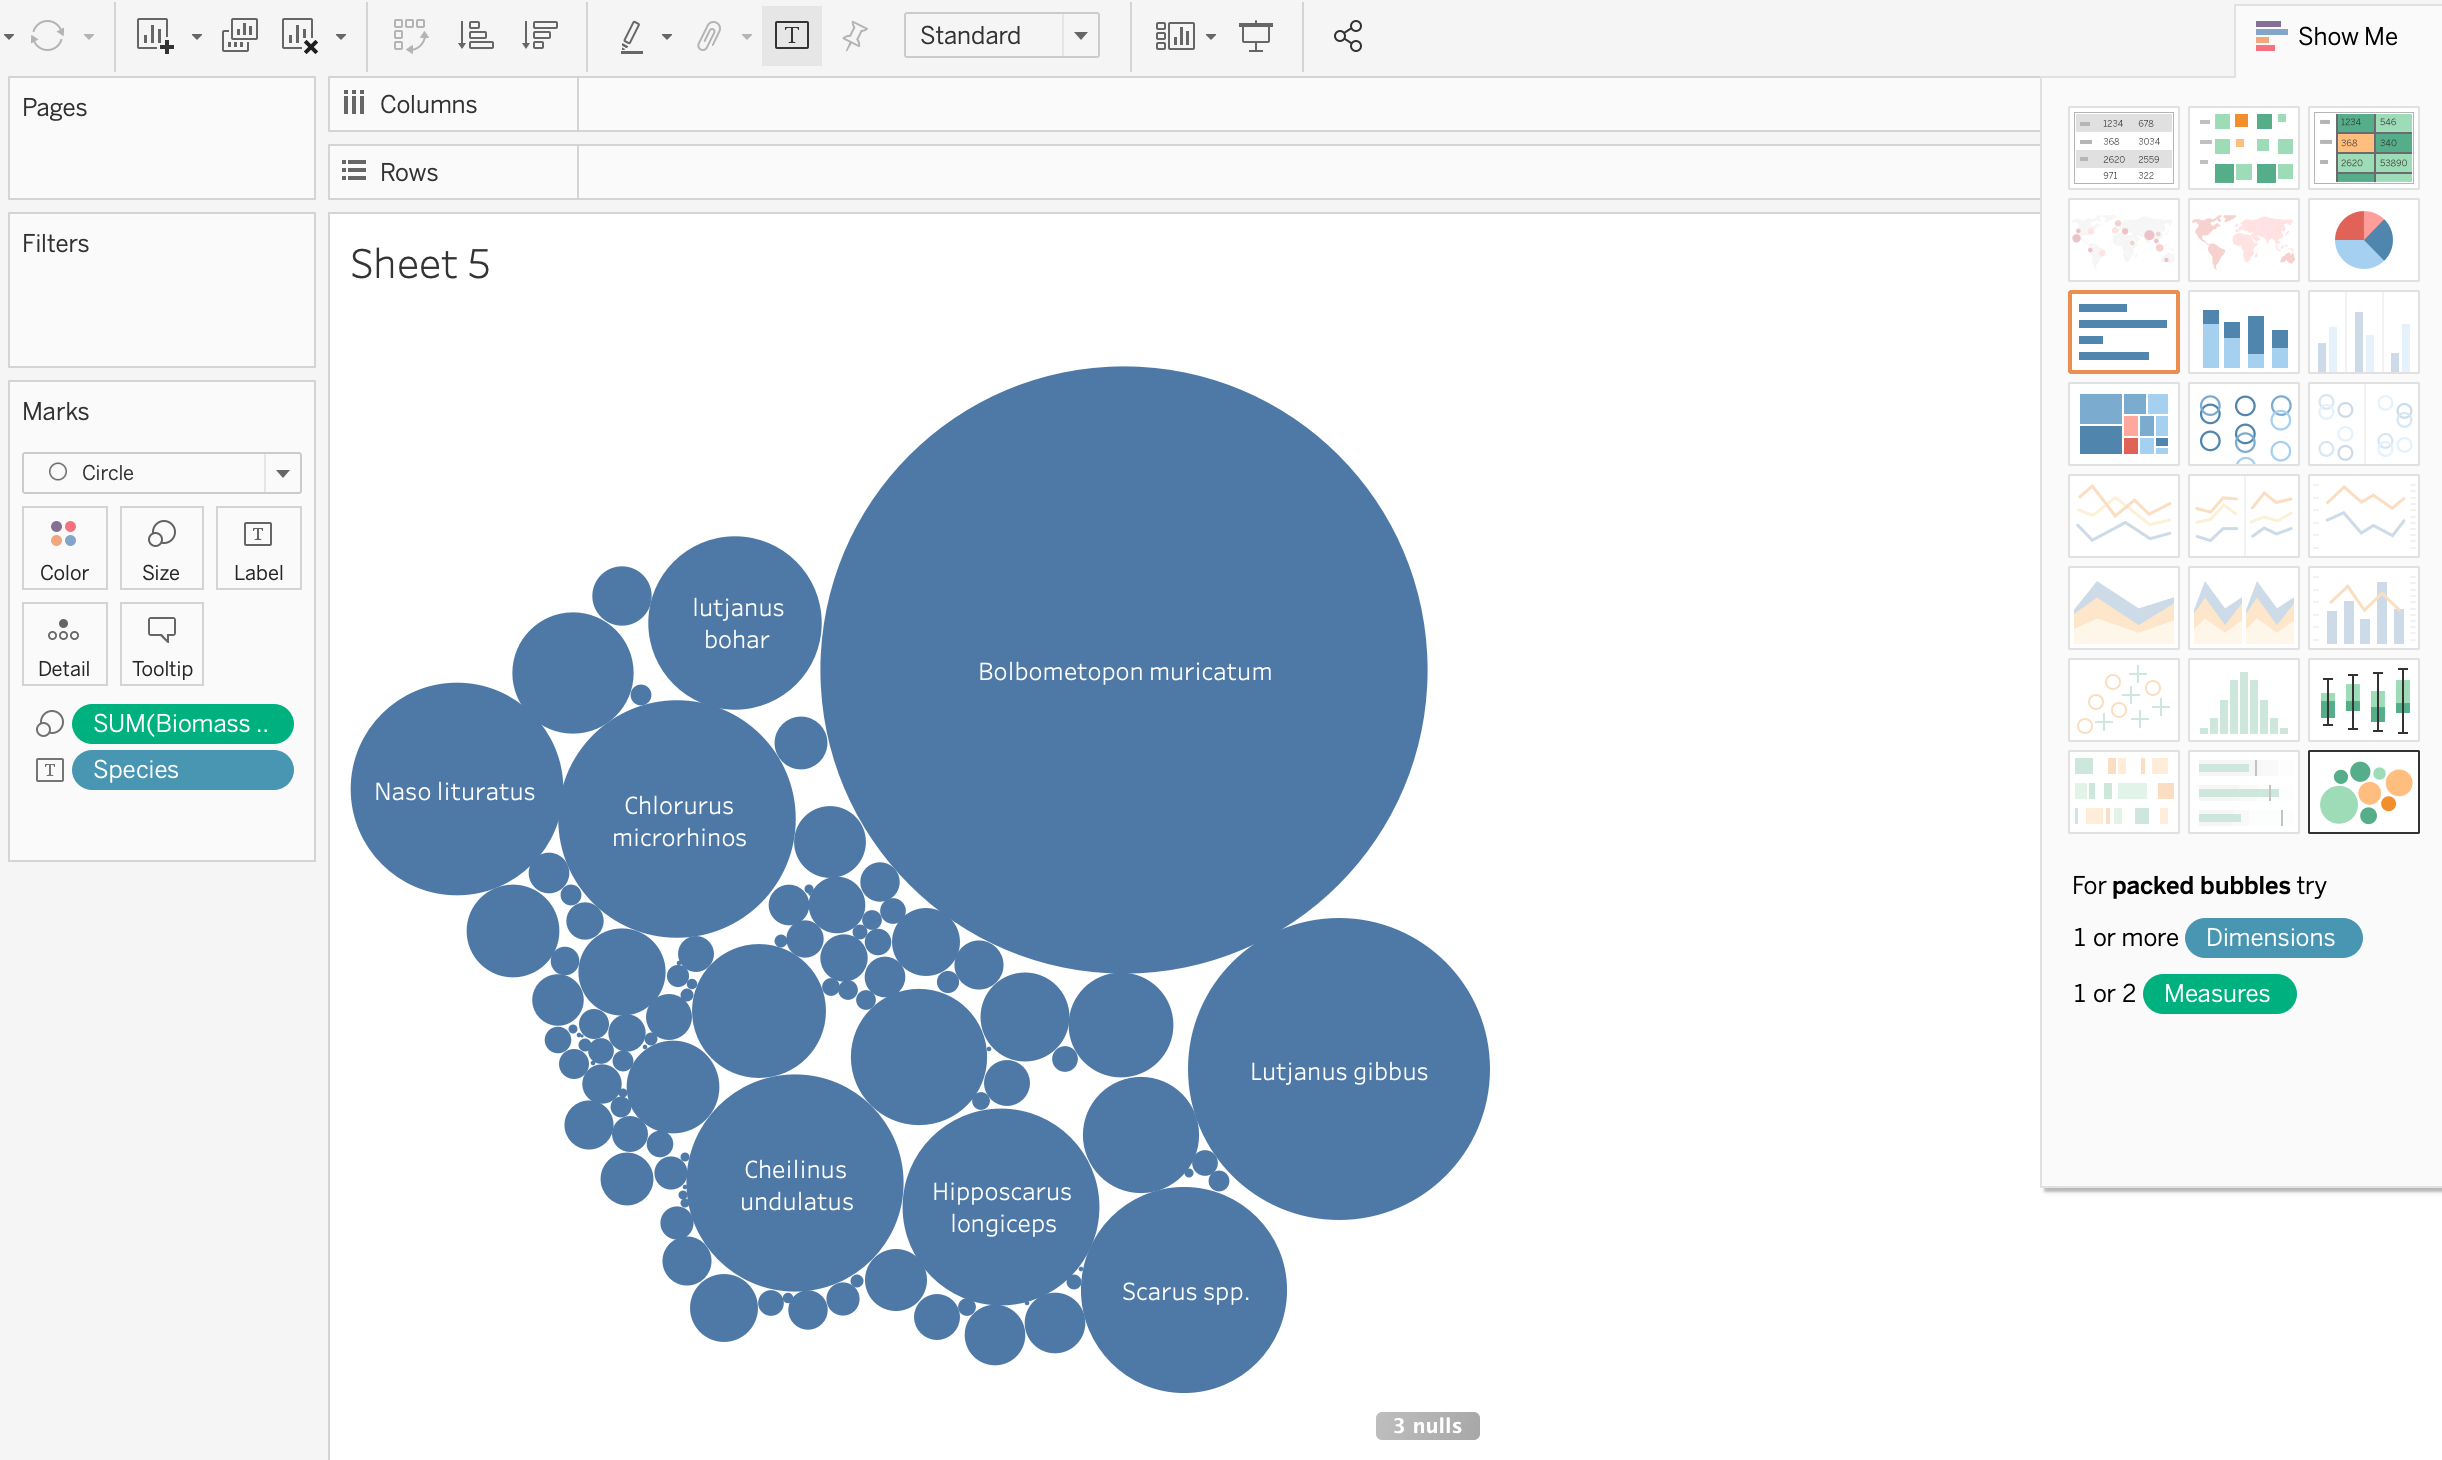
\includegraphics{images/M3S2_bubble-plot.png}
  \item
    Name this sheet ``Bubble.''
  \end{itemize}
\end{enumerate}

\hypertarget{scatter-plot}{%
\subsection{Scatter plot}\label{scatter-plot}}

\begin{enumerate}
\def\labelenumi{\arabic{enumi}.}
\tightlist
\item
  Finally, let's create a Scatter plot. Scatter plots are tricky; follow along with this video to learn about scatter plots in Tableau.
\end{enumerate}

\hypertarget{editing-and-formatting-the-axes}{%
\subsection{Editing and Formatting the Axes}\label{editing-and-formatting-the-axes}}

\begin{enumerate}
\def\labelenumi{\arabic{enumi}.}
\tightlist
\item
  ``Biomass g'' is not a very descriptive title for the x-axis. Let's change it to give more information to a viewer. Double-click on the axis and an editing window will pop up.
\end{enumerate}

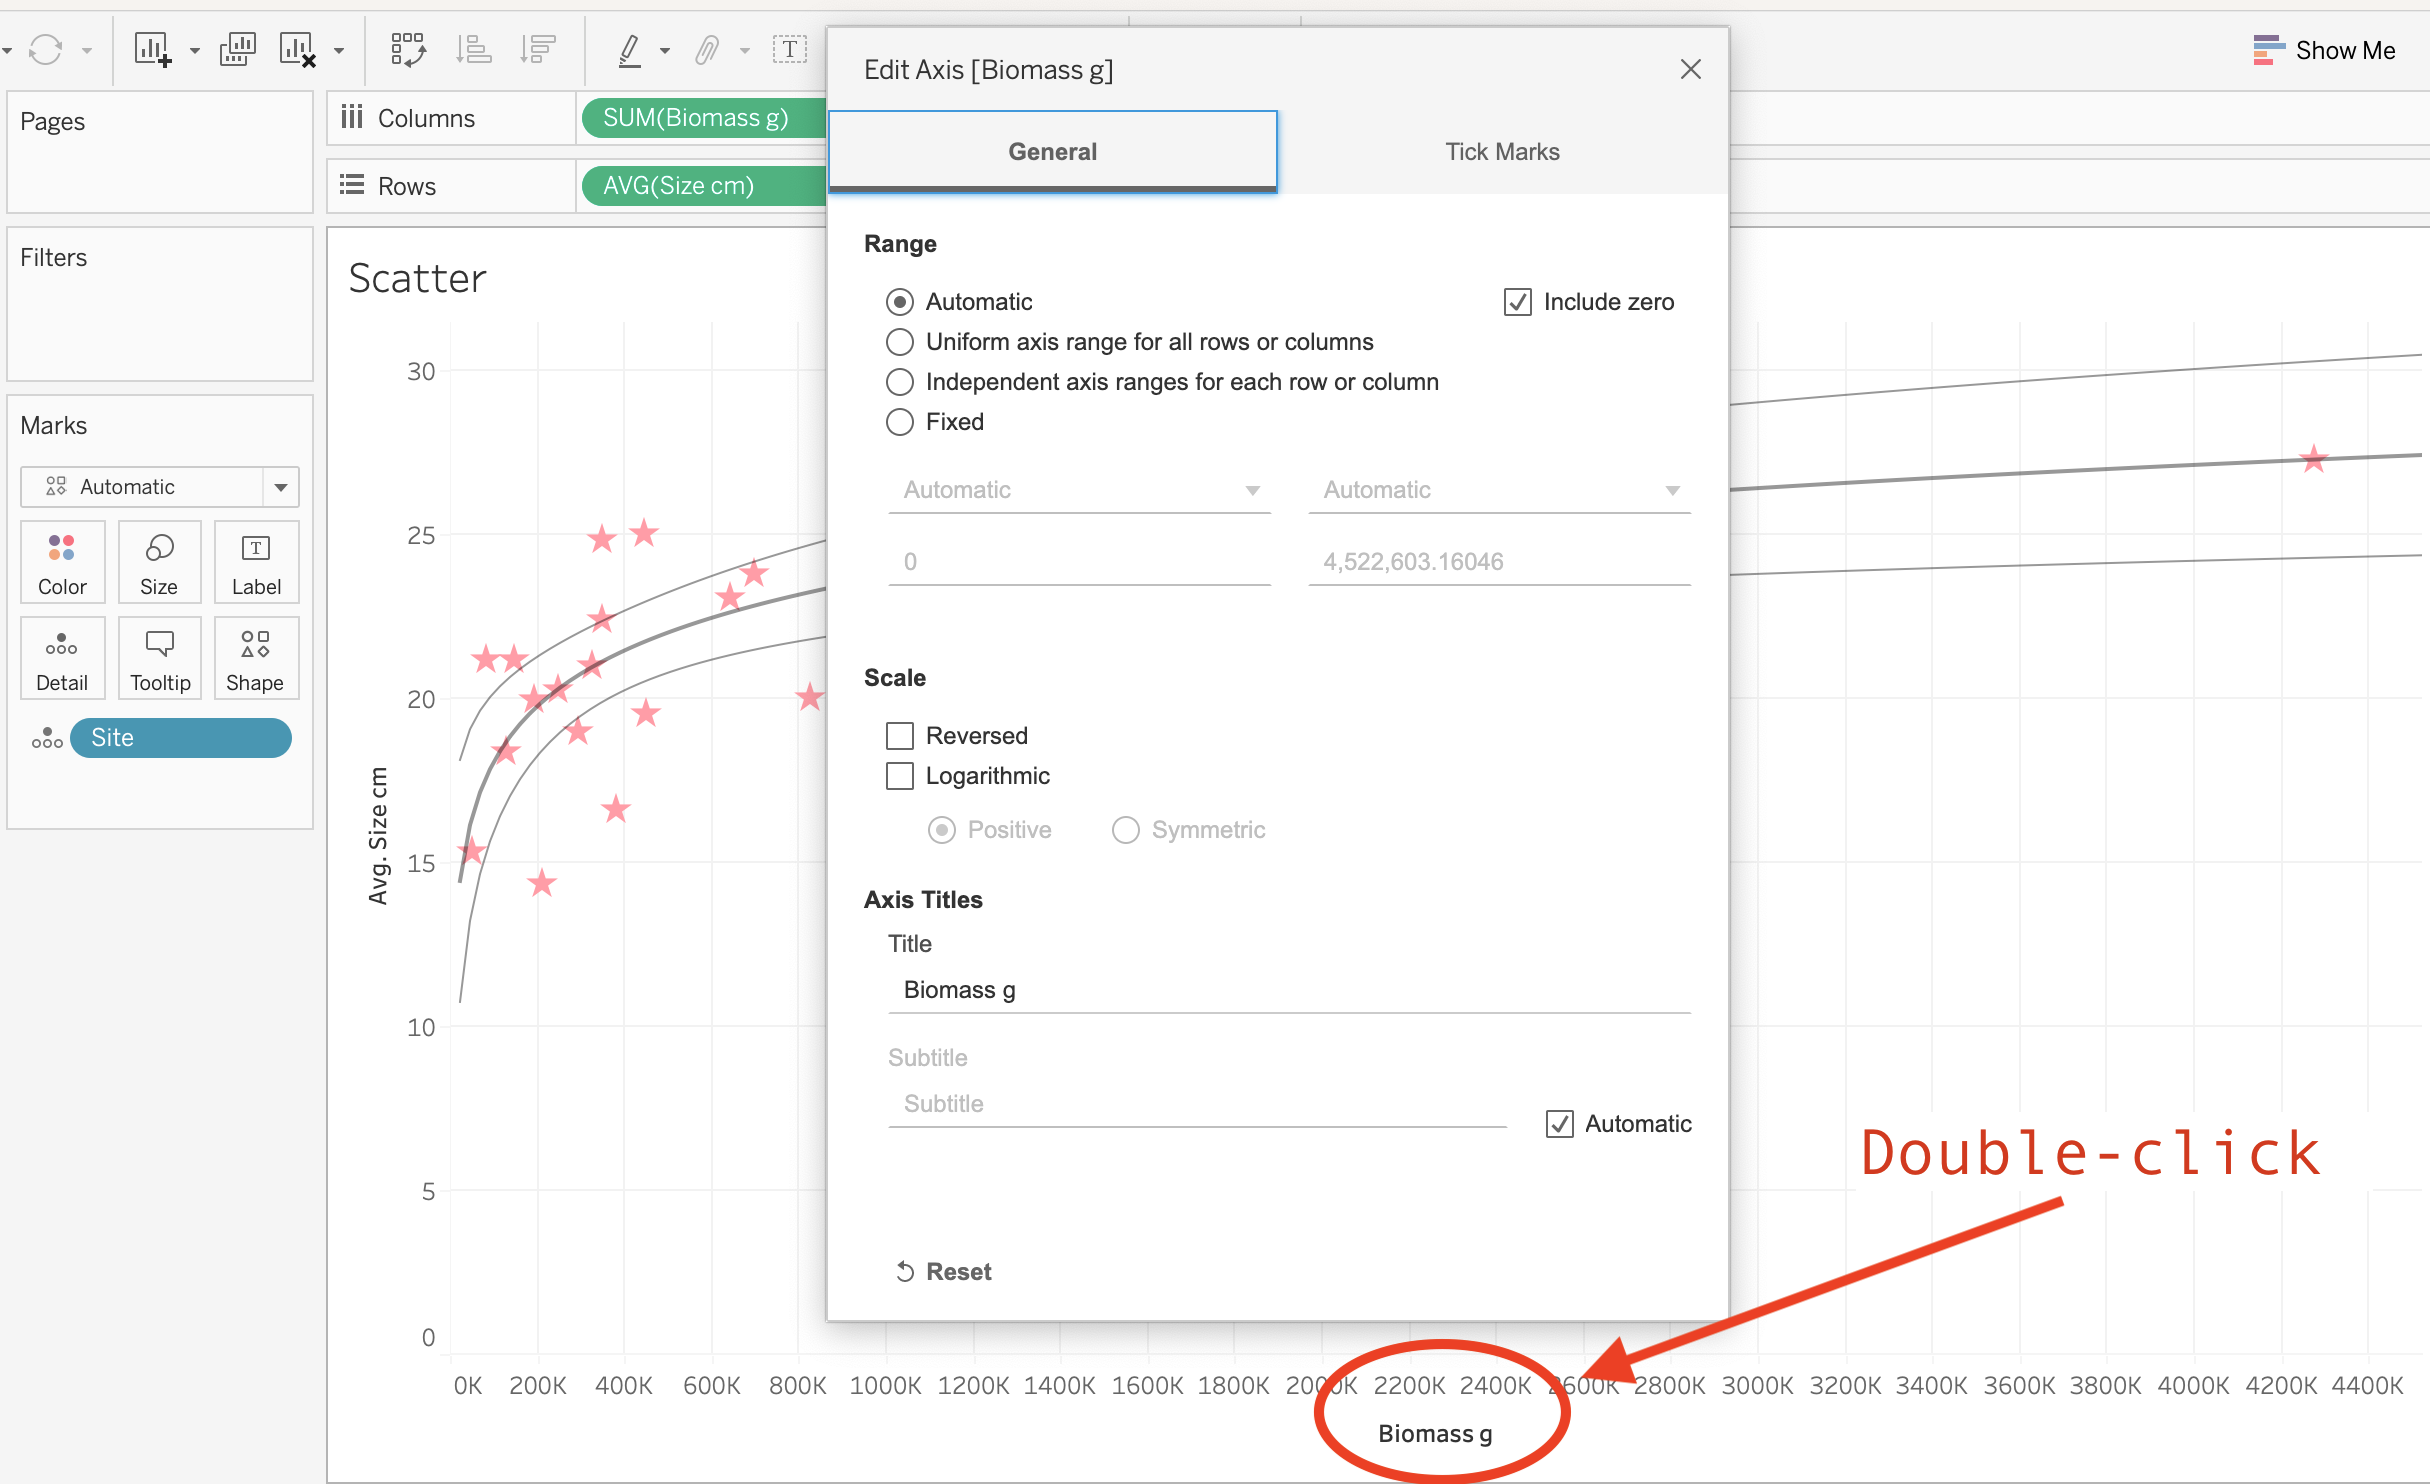
\includegraphics{images/M3S2_edit-axis.png}

\begin{enumerate}
\def\labelenumi{\arabic{enumi}.}
\setcounter{enumi}{1}
\tightlist
\item
  Under Title delete ``Biomass g'' and type ``Total biomass (g).''
\item
  Do the same for the y-axis. Replace the title with ``Avg. Size (cm).''
\item
  Now, we want to increase the font size to make the axes titles easier to read.

  \begin{itemize}
  \item
    Right-click on the y-axis and choose Format.
    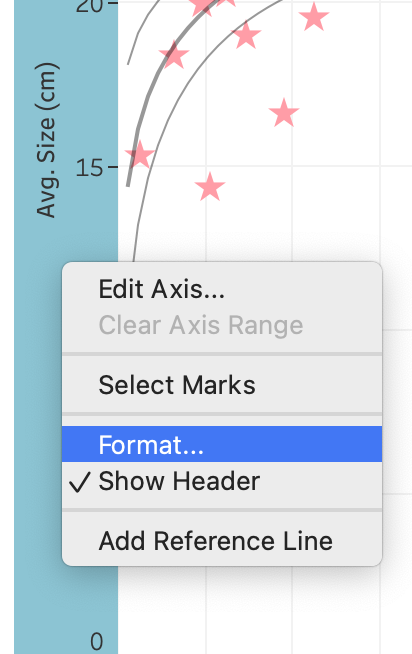
\includegraphics{images/M3S2_format-axis.png}
  \item
    Open the dropdown menu that says Font: and change the font size to 14.
    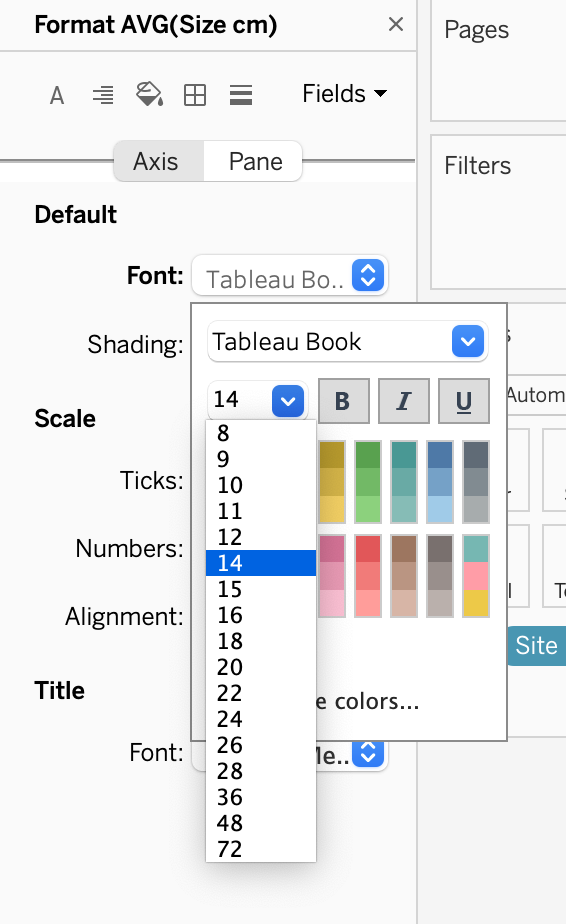
\includegraphics{images/M3S2_axis-font-size.png}
  \end{itemize}
\item
  Do the same for the x-axis.
\item
  When you are done, click on the X in the right corner of the Format window to exit.
\end{enumerate}

\hypertarget{saving-my-files}{%
\subsection{Saving my Files}\label{saving-my-files}}

\begin{enumerate}
\def\labelenumi{\arabic{enumi}.}
\tightlist
\item
  There are two primary ways to save your work in Tableau. The first is similar to saving any other type of file on your computer.

  \begin{itemize}
  \tightlist
  \item
    Click on \textbf{File \textgreater{} Save As} on the menu bar at the top of your screen. Name this file ``Tableau\_class\_skills\_1''. Save the file under your Tableau Data Training folder.
    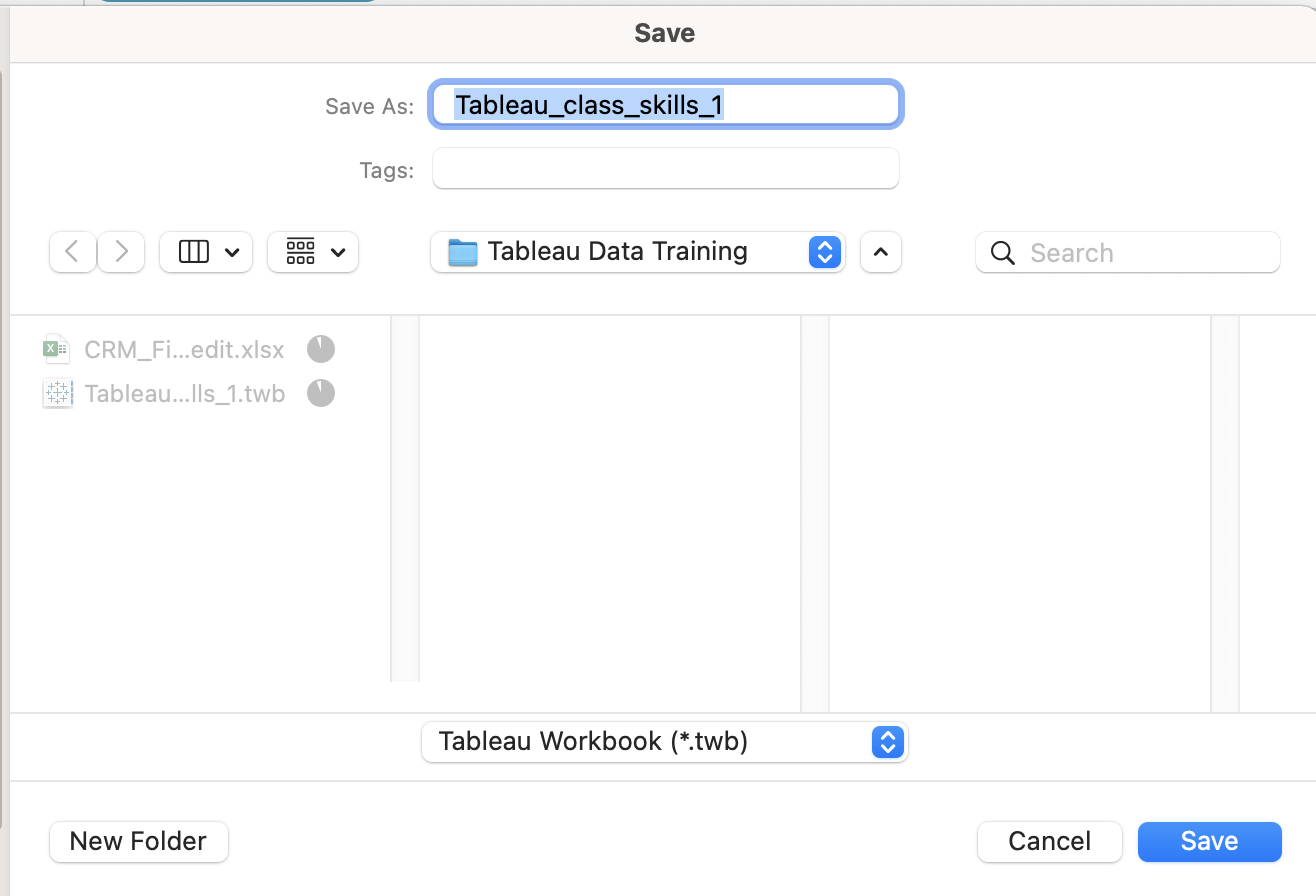
\includegraphics{images/M3S2_save-as.png}
  \item
    Let's take a look at the files. If you look at the Tableau Data Training folder, you'll see that the Excel file CRM\_Fish is 2.1 megabytes while the Tableau Workbook (.twb) that you just saved is 226 kilobytes. That's significantly smaller than the original Excel file because your Tableau Workbook file doesn't contain the data, it just has the instructions for what to do with the data. Therefore if you save .twb files (Tableau Workbook file) and you want to share them with a colleague, you also have to share the original data file.
  \end{itemize}
\item
  Packaged Workbooks

  \begin{itemize}
  \tightlist
  \item
    The second way to save a file saves a compressed version of both the data file and the Tableau Workbook. This is called a Packaged Workbook.
  \item
    First, you have to create a data extract, which puts your data in Tableau format. On the menu bar at the top of your screen click on \textbf{Data \textgreater{} CRM\_Fish \textgreater{} Extract Data}
    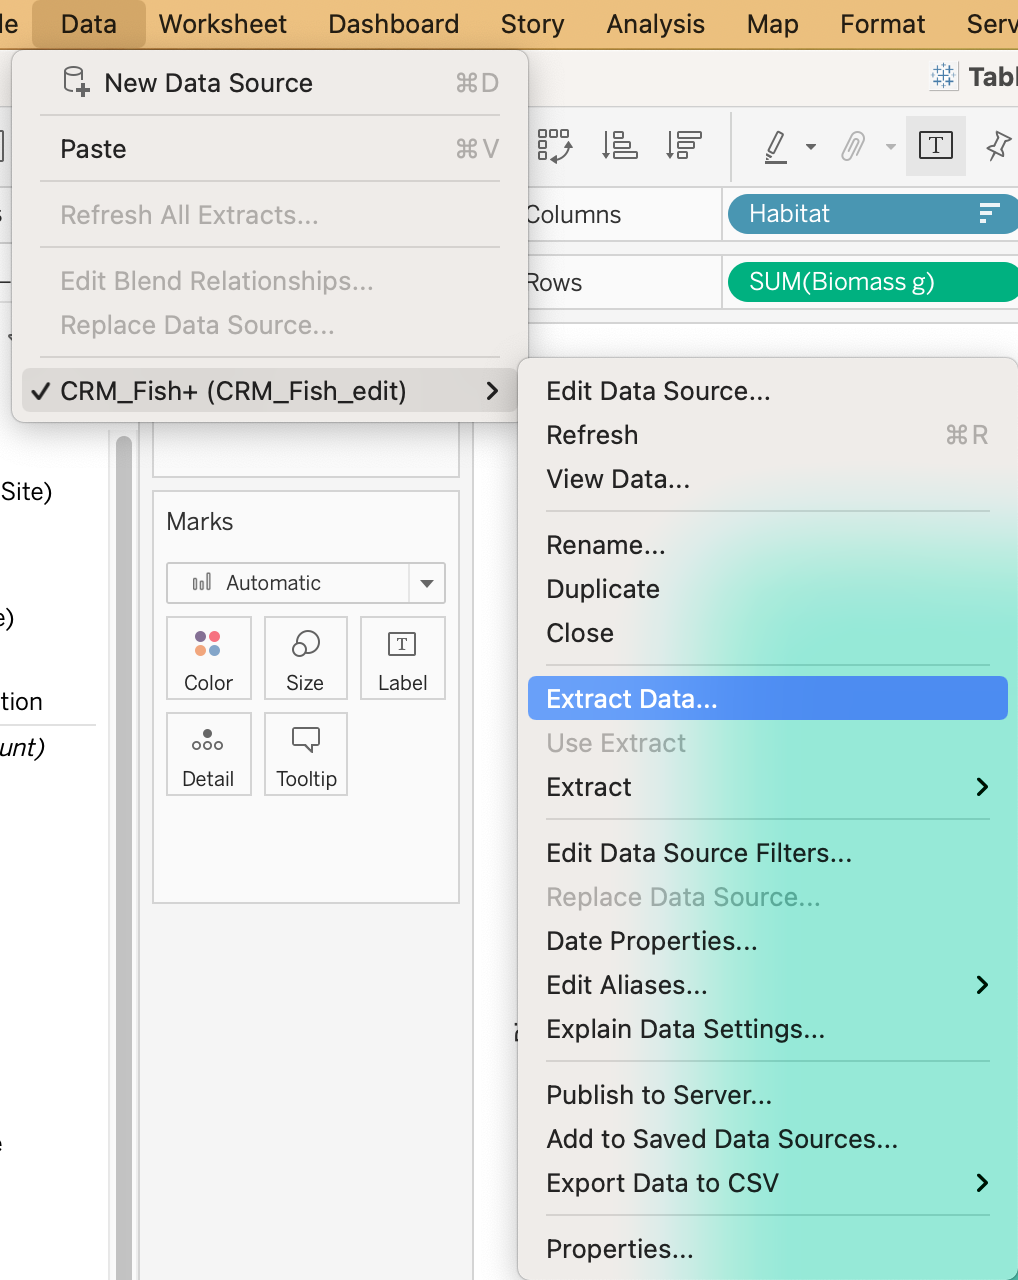
\includegraphics{images/M3S2_extract-data.png}
    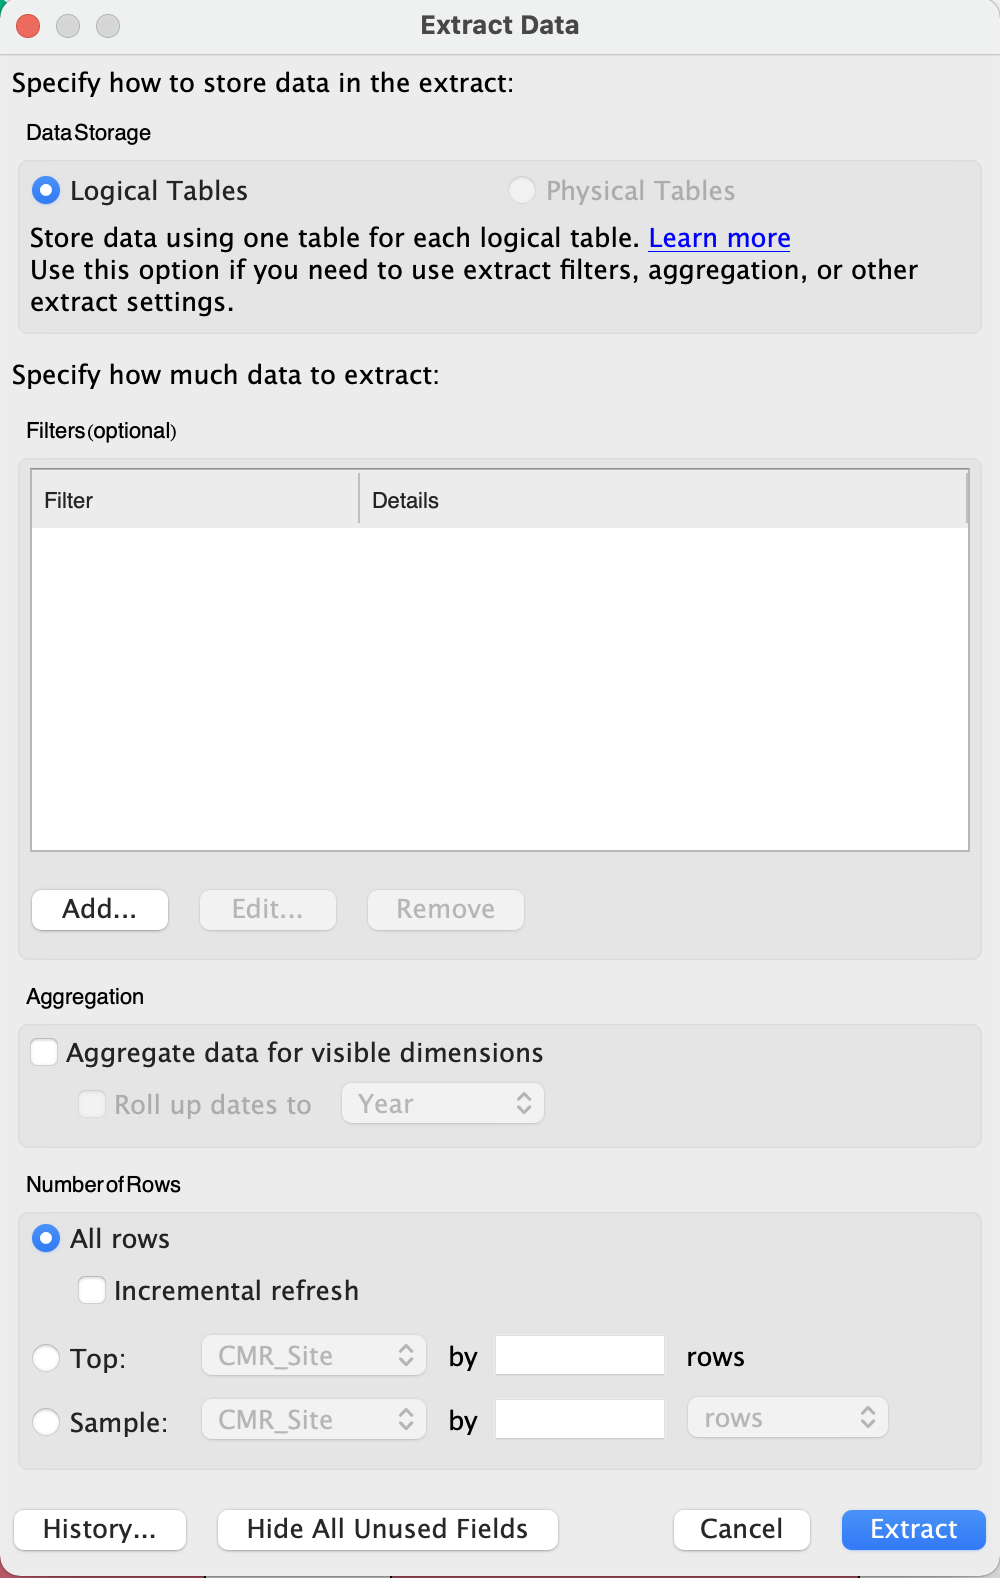
\includegraphics{images/M3S2_extract_menu.png}
  \item
    Click extract, name this file CRM\_Fish\_Extract, and save it in your Tableau Data Training folder.
  \item
    Now that you have created your extract, you will create a packaged file. In order to do that, go to \textbf{File \textgreater{} Export Packaged Workbook \textgreater{} Save}
  \item
    If you look at the folder in your finder, you will see that the new file type is \textbf{.twbx} which means it contains both the data and the instructions (Tableau Packaged Workbook file).
  \item
    If you want to share your work with colleagues who also have Tableau installed, you will share Packaged Workbooks (.twbx) with them.
  \end{itemize}
\end{enumerate}

\hypertarget{homework-exercise}{%
\subsection{Homework Exercise}\label{homework-exercise}}

\begin{enumerate}
\def\labelenumi{\arabic{enumi}.}
\tightlist
\item
  Open data file Excel file CRM\_Fish in Tableau, check field dimensions vs measure, data types, discrete vs.~continuous.
\item
  Create a bar plot, a pie chart, line, map, scatter plot.
\item
  Make presentable for an audience. Ensure that:

  \begin{itemize}
  \tightlist
  \item
    Axes are legible size and descriptive titles
  \item
    Marks utilize nice and legible colors
  \item
    Tooltips provide useful information
  \item
    Name all worksheets
  \end{itemize}
\item
  Create a packaged workbook (.twbx).
\item
  Check your work by comparing it with \href{files/M3S2_exercise_key.twbx}{this file}.
\end{enumerate}

\hypertarget{tableau-skill-part-1-summary}{%
\subsection{Tableau Skill Part 1: Summary}\label{tableau-skill-part-1-summary}}

\begin{enumerate}
\def\labelenumi{\arabic{enumi}.}
\tightlist
\item
  Congratulations! You are now equipped to create basic plots in Tableau and take full control of their design.
\item
  You also know that when sharing your work with colleagues, you should always include the data, either as a separate file, or included in your workbook as a data extract.
\end{enumerate}

\hypertarget{tableau-skills-part-2-multiple-factors-and-dynamic-tables}{%
\section{Tableau Skills Part 2: Multiple factors and dynamic tables}\label{tableau-skills-part-2-multiple-factors-and-dynamic-tables}}

\textbf{\emph{In this session }}

\begin{enumerate}
\def\labelenumi{\arabic{enumi}.}
\tightlist
\item
  \protect\hyperlink{multiple-factors-and-dynamic-tables-learning-objectives}{Learning objectives}
\item
  \protect\hyperlink{multiple-factors-and-dynamic-tables-value-statement}{Value statement}
\item
  \protect\hyperlink{multiple-factor-plots-using-the-marks-menu}{Multiple factor plots using the Marks menu}

  \begin{itemize}
  \tightlist
  \item
    Create a map with multiple factors
  \item
    Create a bar plot with multiple factors
  \item
    Create a timeseries with multiple factors
  \item
    Create a scatter plot with multiple factors
  \item
    Create a bar plot using continuous data
  \end{itemize}
\item
  \protect\hyperlink{maps}{Maps}

  \begin{itemize}
  \tightlist
  \item
    Practice exercise: Search and reset on a Map.
  \end{itemize}
\item
  \protect\hyperlink{filters}{Filters}
\item
  \protect\hyperlink{dynamic-tables}{Dynamic tables}
\item
  \protect\hyperlink{save-your-work}{Save your work}
\item
  \protect\hyperlink{conclusions}{Conclusions}
\item
  \protect\hyperlink{homework}{Homework}
\end{enumerate}

\hypertarget{multiple-factors-and-dynamic-tables-learning-objectives}{%
\subsection{Multiple Factors and Dynamic Tables: Learning objectives}\label{multiple-factors-and-dynamic-tables-learning-objectives}}

\begin{enumerate}
\def\labelenumi{\arabic{enumi}.}
\tightlist
\item
  Learn how to create plots with multiple factors (e.g., colors, mark size, shapes).
\item
  Explore Tableau's mapping functionalities and learn to customize them.
\item
  Understand Tableau's powerful filtering capabilities.
\end{enumerate}

\hypertarget{multiple-factors-and-dynamic-tables-value-statement}{%
\subsection{Multiple Factors and Dynamic Tables: Value statement}\label{multiple-factors-and-dynamic-tables-value-statement}}

\begin{enumerate}
\def\labelenumi{\arabic{enumi}.}
\tightlist
\item
  In this session you will take your skills to the next level and gain full control of how your plots and maps look and how to use filters to display only the information that you are interested in. By adding multiple factors, you can communicate more information through color, size, and shapes. These are the building blocks that make a full interactive visualization!
\end{enumerate}

\hypertarget{multiple-factor-plots-using-the-marks-menu}{%
\subsection{Multiple factor plots using the Marks menu}\label{multiple-factor-plots-using-the-marks-menu}}

\begin{enumerate}
\def\labelenumi{\arabic{enumi}.}
\tightlist
\item
  So far we have learned how to make simple plots, meaning that the plot has one dimension and one measure and you can modify the Marks. But what really makes Tableau awesome is that you can make interactive plots very quickly that look very appealing. Let's start with an example.
\item
  Create a map with multiple factors

  \begin{itemize}
  \tightlist
  \item
    In a new sheet, drag \textbf{Longitude} into \textbf{Columns} and \textbf{Latitude} into \textbf{Rows}. Name the sheet ``Map2''

    \begin{itemize}
    \tightlist
    \item
      Now, let's change the size of the circles to represent the total biomass of that site. In order to make that change, drag and drop the \textbf{Biomass} into the \textbf{Size} in the Marks menu.
    \item
      Result:
      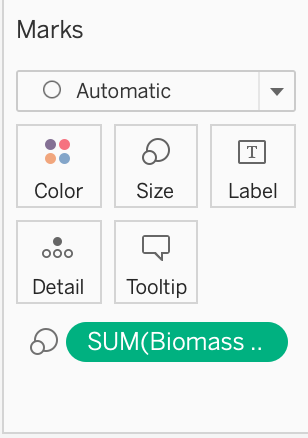
\includegraphics{images/M3S3-Biomass_in_size.png}
      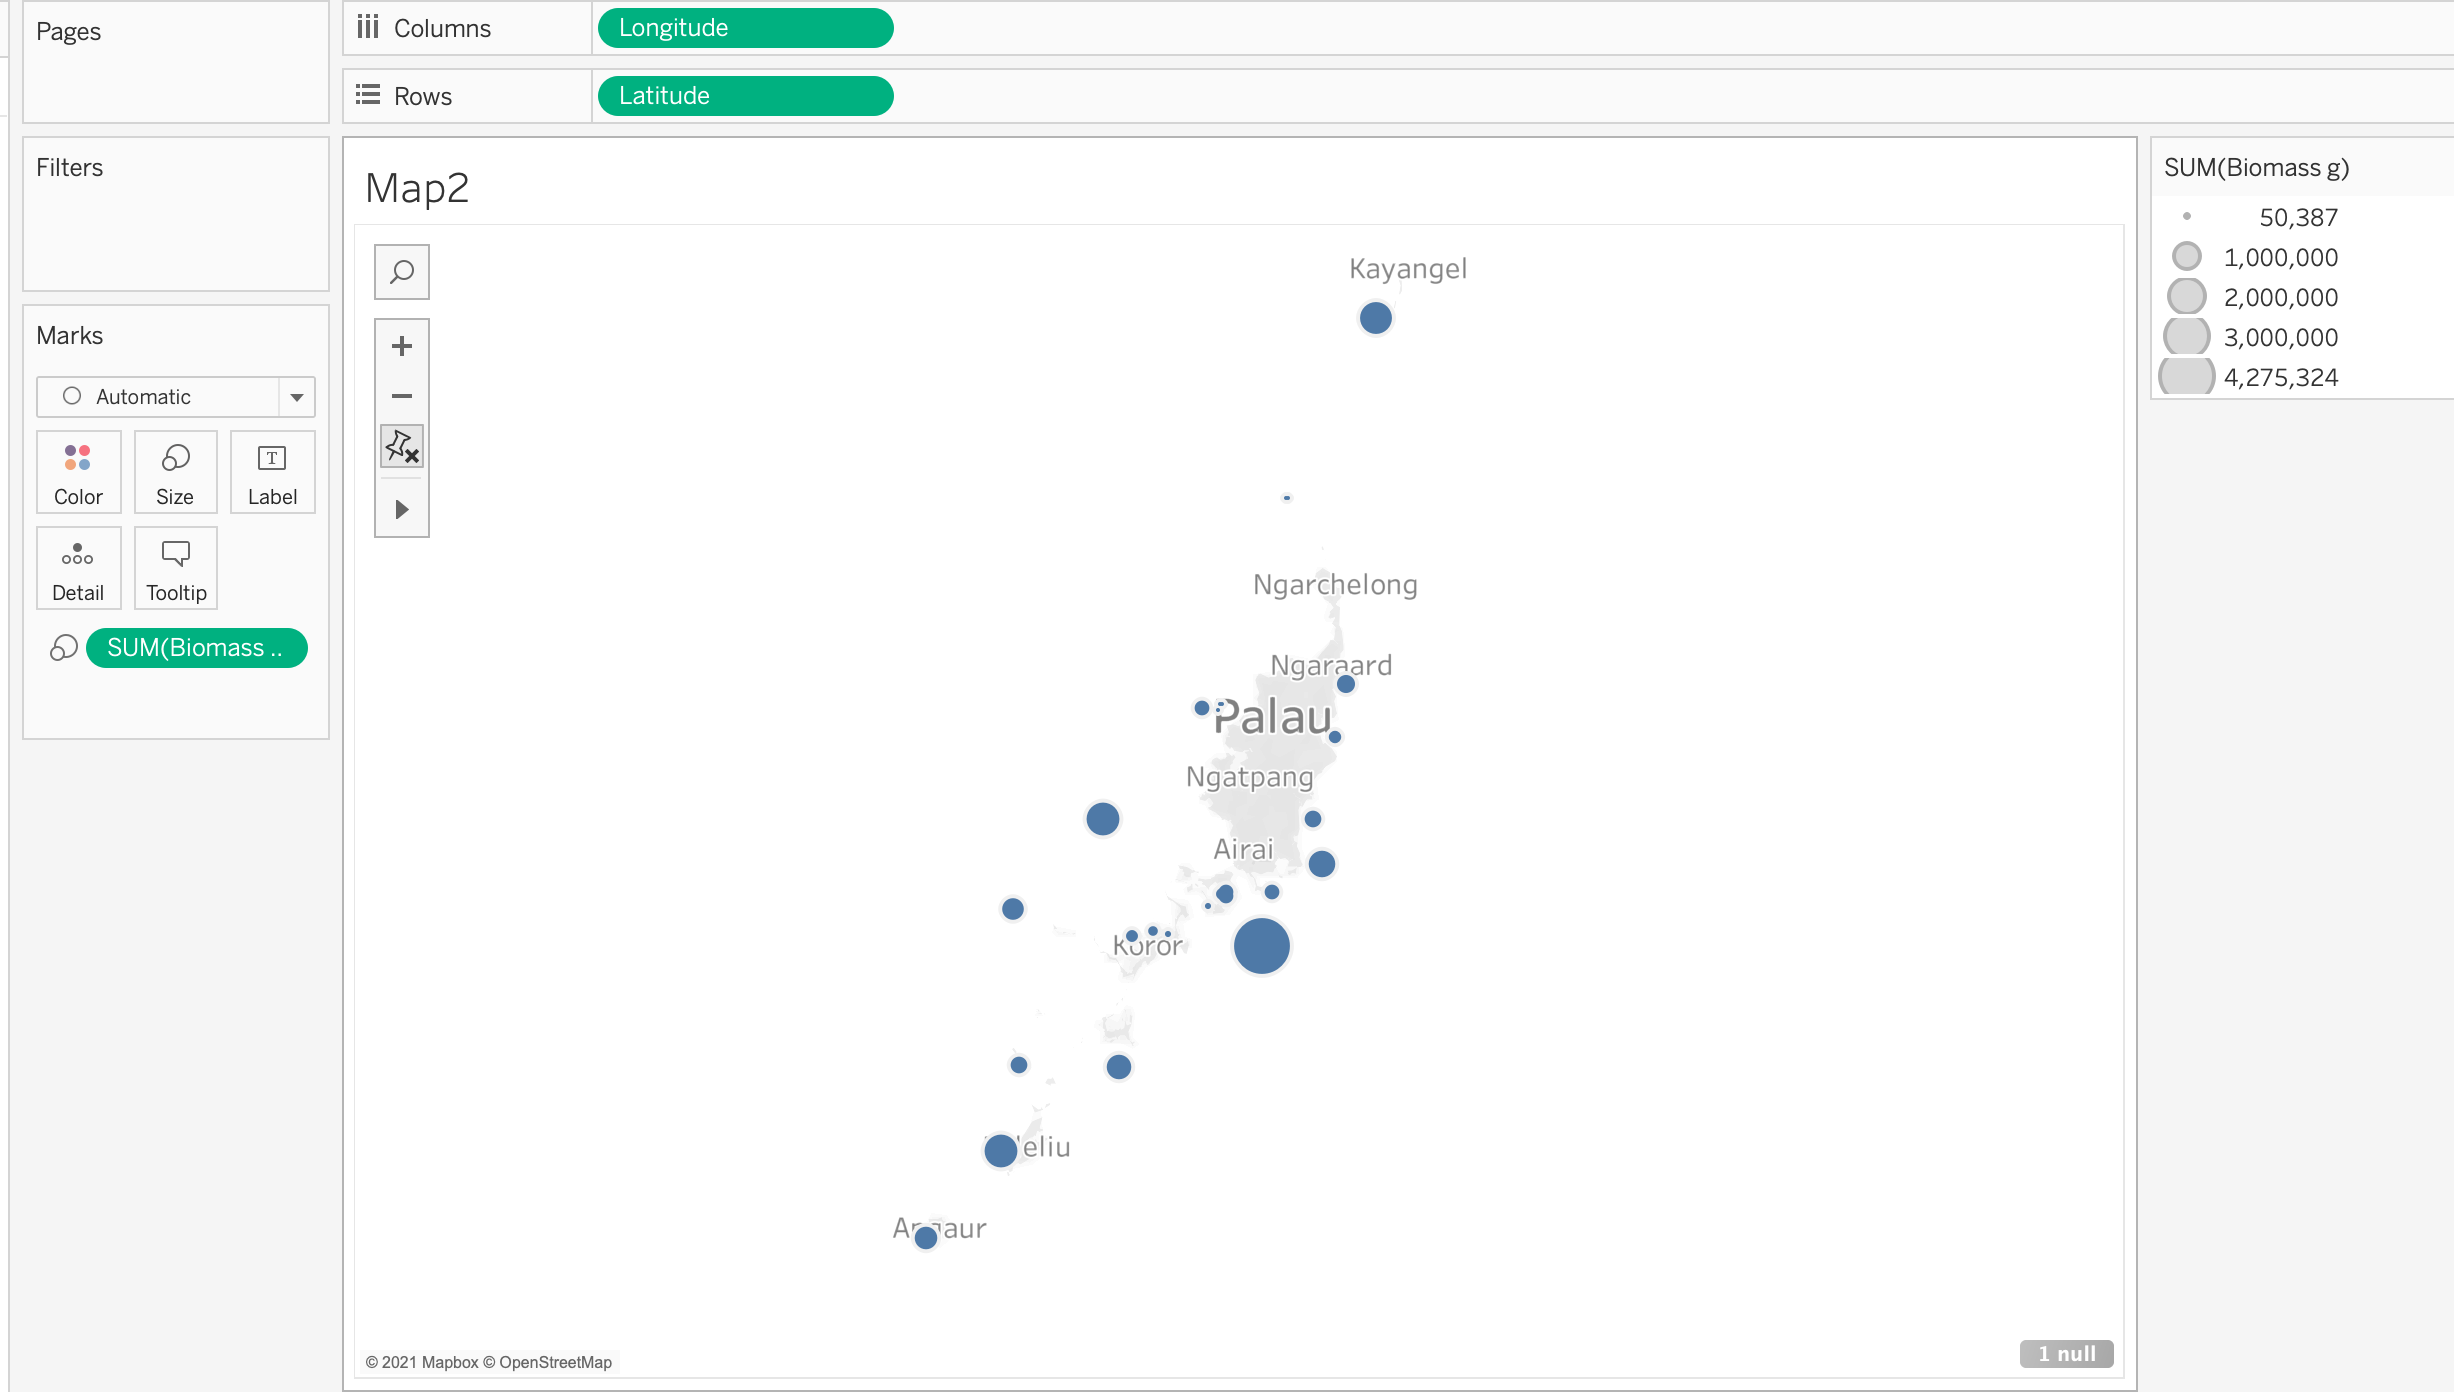
\includegraphics{images/M3S3-map_view_biomass_in_size.png}
    \end{itemize}
  \item
    Troubleshooting: What if I drag something into the wrong Mark?

    \begin{itemize}
    \tightlist
    \item
      \emph{Don't worry, there are 2 easy solutions. First, you can drag the dimension or measure that shows at the bottom of the Mark menu into the correct Mark. Second, you can simply drag the item back into the left column to delete it from the Mark menu. }
    \end{itemize}
  \item
    Exploring the Legend

    \begin{itemize}
    \tightlist
    \item
      In the upper right corner of your Tableau, you should see a legend titled ``SUM(Biomass g)''. If you can't see it, minimize the Show Me menu.
    \item
      If you double-click the legend, you will be able to modify even more aspects of the size marks. Go ahead and play with the ranges to explore.
    \end{itemize}
  \item
    Now, let's say you want to change the color based on the habitat to show the different habitats at different sites on the map. In order to do that, drag and drop Habitat into the Color field of the Marks menu.
  \item
    Double-click the Habitat legend on the right to explore the many color palettes that Tableau offers.

    \begin{itemize}
    \tightlist
    \item
      There are two methods for choosing colors. The first is to just click \textbf{Assign Palette} and Tableau will automatically change the color of each Data Item. The second is to change each color manually. Click on the Data Item, for example \textbf{Inner\_Reef}, so it is highlighted and then click on the specific color you'd like to choose.
    \end{itemize}
  \end{itemize}
\item
  Create a bar plot with multiple factors

  \begin{itemize}
  \tightlist
  \item
    In a new sheet, drag \textbf{Site} into \textbf{Columns} and \textbf{Biomass} into \textbf{Rows}.

    \begin{itemize}
    \item
      Name this sheet ``Bars2''
    \item
      Sort the bars in descending order. There are two potential approaches:

      \begin{itemize}
      \item
        \begin{enumerate}
        \def\labelenumii{\arabic{enumii})}
        \tightlist
        \item
          Right-click the \textbf{Site} item in the Rows field. Click sort and then choose descending and close the pop out menu.
        \end{enumerate}
      \end{itemize}
    \item
      \begin{enumerate}
      \def\labelenumii{\arabic{enumii})}
      \setcounter{enumii}{1}
      \tightlist
      \item
        At the top of Tableau, there is a shortcut menu with many symbols. An explanation of each function should show when you hover over the button. Click this one:
        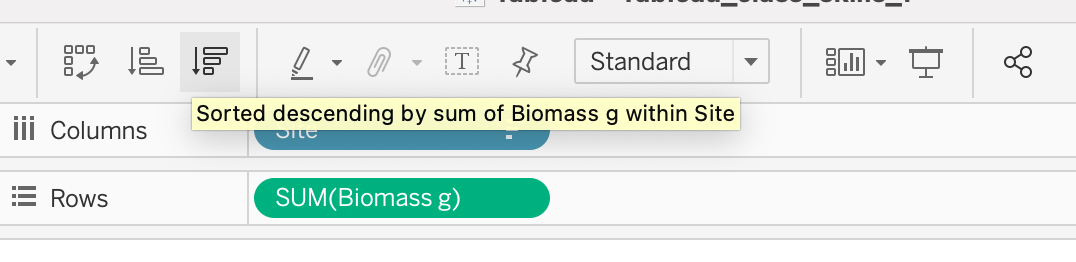
\includegraphics{images/M3S3-sort.png}
      \end{enumerate}

      \begin{itemize}
      \tightlist
      \item
        The arrow pointing down represents descending order.
      \end{itemize}
    \item
      Drag \textbf{Habitat} into the \textbf{Color} mark.
    \end{itemize}
  \item
    You can see that this is the same representation with a bit more detail for a viewer.
  \item
    What if we want to know how different species contribute to the overall biomass of each site?

    \begin{itemize}
    \tightlist
    \item
      Remove \textbf{Habitat} from the Marks menu by dragging it to the left column.
    \end{itemize}
  \item
    This is a fun example of the many possible options you have by adding dimensions and measures into the Marks menu.
  \end{itemize}
\item
  Create a timeseries with multiple factors
\item
  Create a scatter plot with multiple factors

  \begin{itemize}
  \tightlist
  \item
    In a new sheet, drag \textbf{Biomass} into \textbf{Columns} and \textbf{Size} into \textbf{Rows}. Name this sheet ``Scatter2''

    \begin{itemize}
    \tightlist
    \item
      Change the Size from Sum to Average by right-clicking \textbf{Size}, choose \textbf{Measure} and choose \textbf{Average}:
      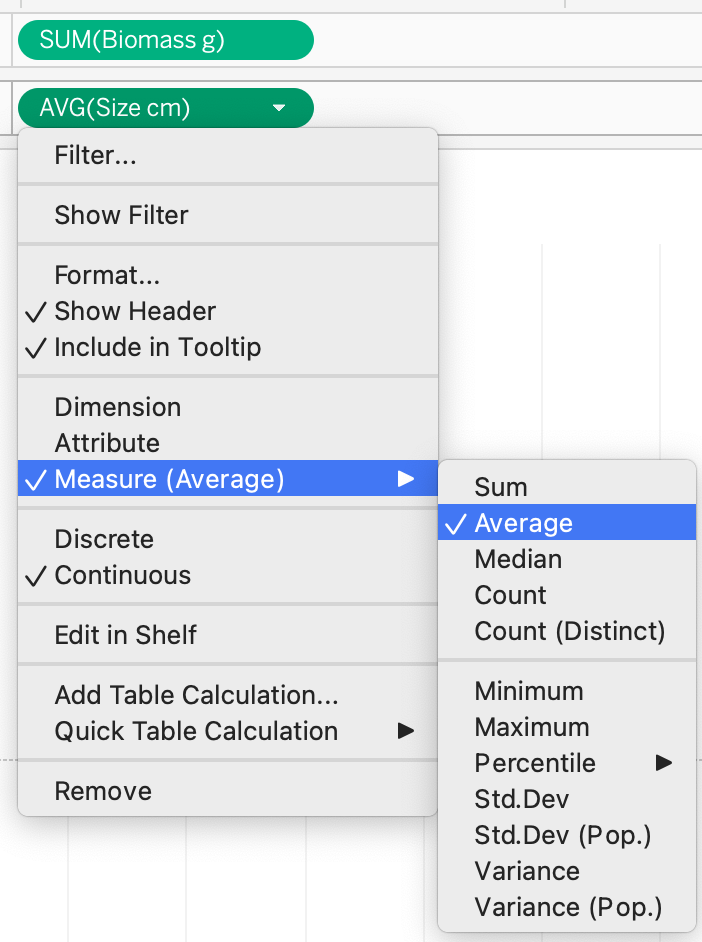
\includegraphics{images/M3S3-scatter-change-size.png}
    \end{itemize}
  \item
    Then, drag \textbf{Site} into \textbf{Details} in the Marks menu.
  \item
    This plot still doesn't give us much information. Let's add more information by changing the shapes of each point on the scatter plot to represent Habitat. Drag \textbf{Habitat} into \textbf{Shapes} in the Marks menu.
  \item
    \emph{Just as you did with Colors, you can double-click Shapes and explore different shape palettes. }
  \item
    Double-click \textbf{Shapes}. Open the drop-down menu under \textbf{Select Shape Palette}: and choose \textbf{Filled}. Then click \textbf{Assign Palette} and \textbf{OK}.
  \item
    What if we want to add even more information? Let's also make each Habitat a different color. To do that, drag a new Habitat field from the left sidebar into \textbf{Color} in the Marks menu.

    \begin{itemize}
    \tightlist
    \item
      \emph{Notice that you have two habitat fields in the Marks menu. }
    \end{itemize}
  \item
    Do you notice that there is blank space at the bottom of the plot from zero to twelve? We don't really need that dead space so let's get rid of it.

    \begin{itemize}
    \tightlist
    \item
      Double-click on the \textbf{y-axis}. Uncheck \textbf{Include zero}. Exit the pop-up screen and you will see that now the plot is much clearer.
    \end{itemize}
  \end{itemize}
\item
  Create a bar plot using continuous data

  \begin{itemize}
  \tightlist
  \item
    So far we have been using discrete data in the Marks menu to customize our plots. What happens when we use continuous data? Let's find out together.
  \item
    In a new sheet, create a bar plot with \textbf{Species} on the x-axis and average \textbf{Size} on the y-axis.

    \begin{itemize}
    \tightlist
    \item
      \emph{Remember that you have to right-click the Size field in Rows to change it from sum to average. }
    \end{itemize}
  \item
    Then sort Species from highest to lowest Size. Right-click the \textbf{Species} field in Columns. Choose \textbf{Sort}.
    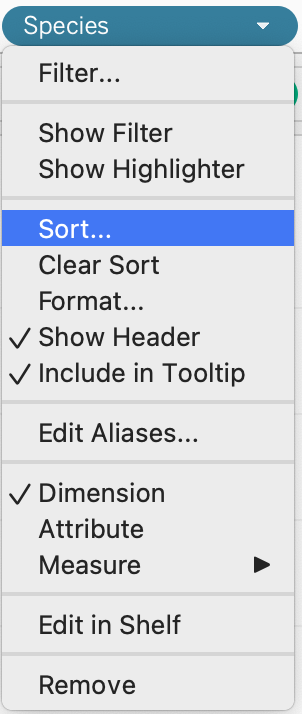
\includegraphics{images/M3S3-bars3-species-sort.png}
  \item
    In the pop-up menu, open the drop-down menu under Sort By, choose \textbf{Field}, and choose \textbf{Descending} under Sort Order.
    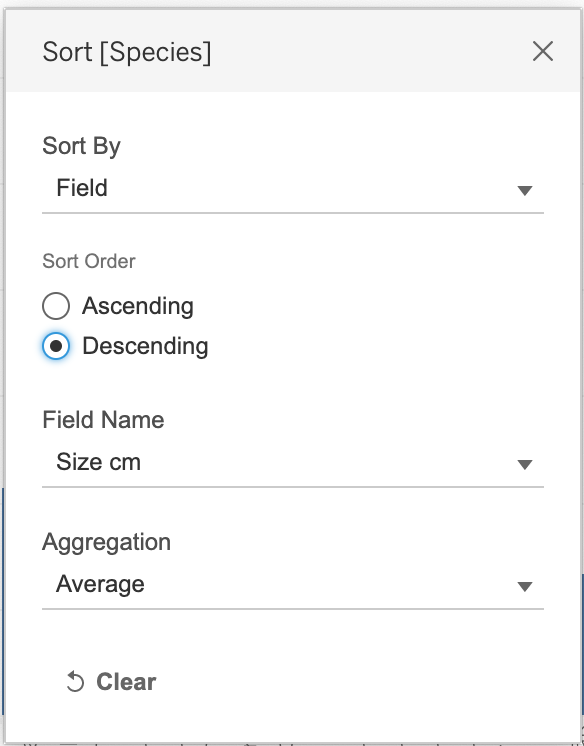
\includegraphics{images/M3S3-bars3-species-sort2.png}

    \begin{itemize}
    \tightlist
    \item
      When you close the pop-up menu, you should see this:
      \includegraphics{images/M3S3-bars3-sort-result.png}
    \end{itemize}
  \item
    What if now we want to know which of these species had the highest observed biomass? One way to do that is to color code the bars by biomass. So drag \textbf{Biomass} to \textbf{Color} in the Marks menu.

    \begin{itemize}
    \tightlist
    \item
      There's a huge outlier. Do you see it?
      \includegraphics{images/M3S3-bars3-outlier.png}
    \end{itemize}
  \item
    Notice that Tableau created a color scale. In previous plots that we made using color to represent discrete data, Tableau automatically created palettes with a set number of colors depending on the number of categories in the data. In this case, Biomass is continuous data so Tableau shows a spectrum of colors to represent the spectrum of continuous data.
  \item
    To change the color palette, double-click on the legend in the upper right corner and explore the palettes that Tableau provides.
  \item
    Right now, the outlier is making it difficult for us to see the difference between other colors. Let's fix that.

    \begin{itemize}
    \tightlist
    \item
      Double-click on the legend and go to \textbf{Advanced \textgreater\textgreater{}}. Check \textbf{End} and change the end field to \textbf{500,000}. Click \textbf{OK}.
      \includegraphics{images/M3S3-bars3-editcolors-advanced.png}
    \end{itemize}
  \item
    Here is the final result:
    \includegraphics{images/M3S3-bars3-final.png}
  \end{itemize}
\end{enumerate}

\hypertarget{maps}{%
\subsection{Maps}\label{maps}}

\begin{enumerate}
\def\labelenumi{\arabic{enumi}.}
\tightlist
\item
  Let's explore the capabilities of maps. In a new sheet, double-click \textbf{Longitude} and \textbf{Latitude} to create a new map. Name this sheet ``Map3''

  \begin{itemize}
  \tightlist
  \item
    Change the color of the points. In the Marks menu, click \textbf{Colors} and choose \textbf{orange}.
  \item
    On the bar at the very top of your screen, you will see that there is a whole menu for Maps. You can go to Background Maps and choose from an array of styles.
    \includegraphics{images/M3S3-map3-menu.png}
  \item
    Open the Map Layers menu. Under \textbf{Maps}, click on \textbf{Map Layers\ldots{}} and a new menu will appear on the left sidebar.

    \begin{itemize}
    \tightlist
    \item
      Under Background choose \textbf{Style: Satellite}.
    \item
      Change \textbf{Washout} to \textbf{20\%}.

      \begin{itemize}
      \tightlist
      \item
        \emph{You can either move the slider right or you can type in the white box.}
      \end{itemize}
    \item
      \emph{The information provided unter Data Layers only applies to the United States. }
    \end{itemize}
  \item
    The map will normally try to occupy the space and show the whole geographic scope of your data as a default. In this case, we see Palau from Kayangel to Angaur.
  \item
    You can also move around the map to explore the whole globe. In the upper left corner of the hover over the triangle and choose Pan:
    \includegraphics{images/M3S3-map3-pan.png}
  \item
    Then, you can click and drag to move the map.
  \item
    You can also choose the options to the right of Pan to use selection tools that allow you to choose a group of points to highlight.
  \item
    You can also zoom in and out using the plus and minus buttons.
  \end{itemize}
\item
  Practice exercise: Search and reset on a Map.

  \begin{itemize}
  \tightlist
  \item
    If you click on the magnifying glass, you can type in different locations to search. For example, you can search for San Diego, California and the map will show you:
    \includegraphics{images/M3S3-map3-SanDiego.png}

    \begin{itemize}
    \tightlist
    \item
      You can also search for the postal code of some countries.
    \end{itemize}
  \item
    Now, your turn. \textbf{Search for your hometown}. How far can you \textbf{zoom in}?
  \item
    Say we want to return to the original view. Click on the button that looks like a thumbtack to \textbf{Reset Map}.
  \end{itemize}
\item
  Another interesting feature of maps in Tableau is that you are not limited to coordinates. For example, your data set can include country names instead.
\end{enumerate}

\hypertarget{filters}{%
\subsection{Filters}\label{filters}}

\hypertarget{dynamic-tables}{%
\subsection{Dynamic Tables}\label{dynamic-tables}}

\begin{enumerate}
\def\labelenumi{\arabic{enumi}.}
\tightlist
\item
  The last thing we are going to learn in this session is how to create and use tables.
\item
  There are three conditions to keep in mind when you create a table in Tableau:

  \begin{itemize}
  \tightlist
  \item
    Data should be dragged into Rows because we are following a long format.

    \begin{itemize}
    \tightlist
    \item
      Refer to \protect\hyperlink{data-cleaning-best-practices}{Module 2} to learn more about long versus block format
    \end{itemize}
  \item
    Everything has to be discrete because the software will always attempt to plot continuous data as a chart, not as text.
  \item
    You can use filters, sort, and all the other functionalities that you learned for other types of plots. Tables in Tableau are similar to dynamic tables in Excel.
  \end{itemize}
\end{enumerate}

\hypertarget{save-your-work}{%
\subsection{Save your work}\label{save-your-work}}

\includegraphics{images/M3S3-save-work.png}

\hypertarget{conclusions}{%
\subsection{Conclusions}\label{conclusions}}

\begin{enumerate}
\def\labelenumi{\arabic{enumi}.}
\tightlist
\item
  Congratulations! You have completed one of the most important sections of this training to be able to fully customize your visualizations in Tableau. By putting together all the pieces that you have learned so far, you are ready to dive into how to make interactive visualizations to share with others. Yet before that step, our next session will teach you how to create new calculated fields to enhance the insights that you can get from your data.
\end{enumerate}

\hypertarget{homework}{%
\subsection{Homework}\label{homework}}

\begin{enumerate}
\def\labelenumi{\arabic{enumi}.}
\tightlist
\item
  Create a bar plot where x-axis is year, y-axis is total biomass, and color is habitat.
\item
  Create a map where size of bubbles represents avg size of fish and color of bubble represents total biomass.
\item
  Create a scatter plot where x-axis is total biomass, y-axis is avg size. Dots represent sites. Color and shape are the year.
\item
  Challenge: Pie chart where color represents habitat, size of slice represents total biomass, 1 pie chart in the same plot for each year 2012, 2013, 2014.
\item
  Create filters for species that allow you to select 1 species at a time in a single dropdown menu for any of these graphs.

  \begin{itemize}
  \tightlist
  \item
    Note: Make sure all axes, labels, tooltips are legible and look presentable for an audience.
  \end{itemize}
\item
  Create a packaged workbook (.twbx).
\item
  Check your work by comparing it with \href{files/M3S3_exercise_key.twbx}{this file}.
\end{enumerate}

\hypertarget{tableau-skills-part-3-operations-and-calculated-fields}{%
\section{Tableau Skills Part 3: Operations and calculated fields}\label{tableau-skills-part-3-operations-and-calculated-fields}}

\textbf{\emph{In this session}}

\begin{enumerate}
\def\labelenumi{\arabic{enumi}.}
\tightlist
\item
  \protect\hyperlink{operations-and-calculated-fields-learning-objectives}{Learning objectives}
\item
  \protect\hyperlink{operations-and-calculated-fields-value-statement}{Value statement}
\item
  \protect\hyperlink{convert-units-using-calculated-fields}{Convert units using Calculated Fields}
\item
  \protect\hyperlink{manually-calculate-average}{Manually calculate average}
\item
  \protect\hyperlink{more-functions}{More functions}
\item
  \protect\hyperlink{table-calculations-percentage-of-total-and-running-total}{Table calculations: percentage of total and running total}
\item
  \protect\hyperlink{operations-and-calculated-fields-conclusions}{Conclusions}
\end{enumerate}

\hypertarget{operations-and-calculated-fields-learning-objectives}{%
\subsection{Operations and calculated fields: Learning objectives}\label{operations-and-calculated-fields-learning-objectives}}

\begin{enumerate}
\def\labelenumi{\arabic{enumi}.}
\tightlist
\item
  Learning the different ways to calculate custom fields in Tableau.
\item
  Using new calculations to extract new insights from data.
\end{enumerate}

\hypertarget{operations-and-calculated-fields-value-statement}{%
\subsection{Operations and calculated fields: Value statement}\label{operations-and-calculated-fields-value-statement}}

\begin{enumerate}
\def\labelenumi{\arabic{enumi}.}
\tightlist
\item
  In this session you will learn how to create new calculated fields in tableau, ranging from simple sums and averages, to more complex operations such as running totals and percentages.
\end{enumerate}

\hypertarget{convert-units-using-calculated-fields}{%
\subsection{Convert units using Calculated Fields}\label{convert-units-using-calculated-fields}}

\begin{enumerate}
\def\labelenumi{\arabic{enumi}.}
\tightlist
\item
  So far we have mostly used measures to create plots by using SUM and AVERAGE. In certain situations, however, we might need to perform some operations by using one or more variables or calculate a new field. In the example below you will see how these calculated fields can be used to change a value from grams to tonnes.
\end{enumerate}

\hypertarget{manually-calculate-average}{%
\subsection{Manually calculate average}\label{manually-calculate-average}}

\begin{enumerate}
\def\labelenumi{\arabic{enumi}.}
\tightlist
\item
  While Tableau provides an easy way to calculate the AVERAGE through using the right click functionalities on a field that is being used in an active chart, there are other ways to estimate it manually, and with more control over what the software is doing. The video below shows how to do this and how it compares to Tableau's automatic method.
\end{enumerate}

\hypertarget{more-functions}{%
\subsection{More functions}\label{more-functions}}

\begin{enumerate}
\def\labelenumi{\arabic{enumi}.}
\tightlist
\item
  While we have covered the basics of how to create calculated fields, there is a lot more to explore.
\item
  Open a new \textbf{Calculated Field} and click on the small arrow on the right to expand the menu.
  \includegraphics{images/m3s4_open-functions.png}
  \includegraphics{images/m3s4_view-functions.png}
\item
  If you scroll through the list, you will see all the functions that Tableau is capable of performing. These functions are very similar to operations and columns in Excel.
\item
  We recommend that you check out Tableau's free online resources to learn more about calculated fields.

  \begin{itemize}
  \tightlist
  \item
    \href{https://www.tableau.com/learn/training/20212}{Tableau free training videos}
  \item
    Or if you are looking for tips not provided by Tableau, make sure that you are searching for operations in SQL language.
  \end{itemize}
\item
  One common calculation in ecology is finding the average biomass at a site that has been sampled multiple times, such as by several divers each swimming transects. You can use a calculated field, yet the details of your sampling and data arrangement affect how you set it up. See an example of setting up a calculated field in the sample data set below.
\end{enumerate}

\hypertarget{table-calculations-percentage-of-total-and-running-total}{%
\subsection{Table calculations: percentage of total and running total}\label{table-calculations-percentage-of-total-and-running-total}}

\begin{enumerate}
\def\labelenumi{\arabic{enumi}.}
\item
  One additional way to perform custom calculations is by using Table calculations, which are affected explicitly by whatever is being displayed in the active chart.
\item
  In order to understand these better, let's do an example. Create a new pie chart.

  \begin{itemize}
  \tightlist
  \item
    Create a new sheet and name it ``Pie4.''
  \item
    Drag \textbf{Habitat} into \textbf{Columns} and \textbf{Biomass tonnes} into \textbf{Rows}.

    \begin{itemize}
    \tightlist
    \item
      \emph{A bar chart will appear }.
    \end{itemize}
  \item
    Open the \textbf{Show Me} menu and choose \textbf{pie charts}.
  \item
    Change the view to Entire View.
  \item
    Activate labels by clicking on \textbf{Label} in the Marks menu and check \textbf{Show mark labels} and change the font size to 14pt.
    \includegraphics{images/m3s4_pie-show-labels.png}
  \end{itemize}
\item
  Next, follow along as Alfredo shows you how to calculate percentages of total and display them in the labels.
\item
  Just like with Calculated Fields, Table Calculations are a powerful tool in Tableau's repository. If you want to explore more resources, go to:

  \begin{itemize}
  \tightlist
  \item
    \url{https://help.tableau.com/current/pro/desktop/en-us/calculations_tablecalculations.htm}
  \end{itemize}
\end{enumerate}

\hypertarget{operations-and-calculated-fields-conclusions}{%
\subsection{Operations and calculated fields: Conclusions}\label{operations-and-calculated-fields-conclusions}}

\begin{enumerate}
\def\labelenumi{\arabic{enumi}.}
\tightlist
\item
  Great work! You have completed the section on how to create your own calculations and use them to enhance your understanding of the data through visualizations. You are now ready to put all of these elements together and dive right into the creation of dashboards.
\end{enumerate}

\hypertarget{tableau-dashboards-part-1-basic-dashboards}{%
\section{Tableau Dashboards Part 1: Basic dashboards}\label{tableau-dashboards-part-1-basic-dashboards}}

\textbf{\emph{In this session}}

\begin{enumerate}
\def\labelenumi{\arabic{enumi}.}
\tightlist
\item
  \protect\hyperlink{basic-dashboards-learning-objectives}{Learning objectives}
\item
  \protect\hyperlink{basic-dashboards-value-statement}{Value statement}
\item
  \protect\hyperlink{introduction-to-dashboards}{Introduction to dashboards}
\item
  \protect\hyperlink{floating-dashboards}{Floating dashboards}
\item
  \protect\hyperlink{actions-filter-and-highlight}{Actions: filter and highlight}
\item
  \protect\hyperlink{basic-dashboards-conclusions}{Conclusions}
\item
  \protect\hyperlink{basic-dashboards-homework}{Homework}
\end{enumerate}

\hypertarget{basic-dashboards-learning-objectives}{%
\subsection{Basic dashboards: Learning objectives}\label{basic-dashboards-learning-objectives}}

\begin{enumerate}
\def\labelenumi{\arabic{enumi}.}
\tightlist
\item
  Learn the basic windows and menus to create dashboards.
\item
  Explore how to make different charts interact with each other through dashboard actions.
\end{enumerate}

\hypertarget{basic-dashboards-value-statement}{%
\subsection{Basic dashboards: Value statement}\label{basic-dashboards-value-statement}}

\begin{enumerate}
\def\labelenumi{\arabic{enumi}.}
\tightlist
\item
  In this session, you will jump from creating individual charts, to creating dashboards where you can combine multiple charts and make them interact with each other.
\item
  You will also learn the basics for how to make your visualizations more visually appealing through the customization of colors, positions, legends, and other visual elements.
\end{enumerate}

\hypertarget{introduction-to-dashboards}{%
\subsection{Introduction to dashboards}\label{introduction-to-dashboards}}

\begin{enumerate}
\def\labelenumi{\arabic{enumi}.}
\tightlist
\item
  The very first thing to learn about dashboards is how to add different elements to it. Not everything is about the interactive charts, but also the text, symbols and other elements that help you convey a story for the reader. In the video below, you will learn how to set up your canvas and add elements to it.
\end{enumerate}

\hypertarget{floating-dashboards}{%
\subsection{Floating dashboards}\label{floating-dashboards}}

\begin{enumerate}
\def\labelenumi{\arabic{enumi}.}
\tightlist
\item
  Another important skill to master is the correct positioning of the elements in a dashboard. While Tableau tries to help with a tiled arrangement (as in the video above), it is important that you know how to gain full control of the exact size and position of each item that you add. The video below will help you get familiar with these important skills.
\item
  Remember that when working with graphic designers, managing sizes and positions is extremely important. Make sure to practice these skills.
\end{enumerate}

\hypertarget{actions-filter-and-highlight}{%
\subsection{Actions: filter and highlight}\label{actions-filter-and-highlight}}

\begin{enumerate}
\def\labelenumi{\arabic{enumi}.}
\tightlist
\item
  Once you have added various elements, and charts, to your dashboards, it is time to make them interact with each other. The video below will show you two methods (filtering and highlighting) to use one chart to control the items in another chart. We will also cover some common troubleshooting situations.
\end{enumerate}

\hypertarget{basics-dashboards-conclusions}{%
\subsection{Basics dashboards: Conclusions}\label{basics-dashboards-conclusions}}

\begin{enumerate}
\def\labelenumi{\arabic{enumi}.}
\tightlist
\item
  Congratulations! You have completed the most important step in moving from single charts, to fully interactive data visualizations. The next step is to enhance these visuals a little more by learning how to incorporate graphic design elements.
\end{enumerate}

\hypertarget{basic-dashboards-homework}{%
\subsection{Basic dashboards: Homework}\label{basic-dashboards-homework}}

\begin{enumerate}
\def\labelenumi{\arabic{enumi}.}
\tightlist
\item
  Create a map.

  \begin{itemize}
  \tightlist
  \item
    Remember that you know how to change the background and edit colors of the dots.
  \end{itemize}
\item
  Create a scatter plot where the x-axis is average size, y-axis is total biomass and each mark within the scatterplot is a different species.
\item
  Now, create a dashboard with the map and the scatterplot. Create a filter so that when you click on the map it filters the scatterplot.

  \begin{itemize}
  \tightlist
  \item
    Remember to include title and text that describes the purpose of the dashboard.
  \item
    Feel free to create a canvas size that fits your taste. If you want a place to start, try 1000x800 (WxH).
  \item
    Pay special attention to the positioning of your elements by using the `layout' menu. Look at the answer key to see the exact positioning that the instructor used.
  \item
    Remember that you can also change the font size and color of any item in the dashboard (including the color legend) by clicking on the particular element and selecing `format'.
  \item
    If you have trouble making the filter work, use the answer key to open up the available action in the Dashboard/Actions menu. Make sure you understand everything that is going on within the action.
  \item
    Finally, remember that you can right click on the titles of each chart and hide them. This might be helpful to streamline the number of titles in the dashboard.
  \end{itemize}
\item
  Try a few adjustments to practice getting the aesthetic feel just the way you want.
\end{enumerate}

\hypertarget{tableau-dashboards-part-2-graphic-design-elements}{%
\section{Tableau Dashboards Part 2: Graphic design elements}\label{tableau-dashboards-part-2-graphic-design-elements}}

\textbf{\emph{In this session }}

\begin{enumerate}
\def\labelenumi{\arabic{enumi}.}
\tightlist
\item
  \protect\hyperlink{graphic-design-learning-objectives}{Learning objectives}
\item
  \protect\hyperlink{graphic-design-value-statement}{Value statement}
\item
  \protect\hyperlink{recap-tooltip-customization-and-exact-colors}{Recap: Tooltip customization and exact colors}
\item
  \protect\hyperlink{background-images}{Background images}
\item
  \protect\hyperlink{custom-shapes}{Custom shapes}
\item
  \protect\hyperlink{filters-in-dashboards}{Filters in dashboards}
\item
  \protect\hyperlink{dynamic-text-elements}{Dynamic text elements}
\item
  \protect\hyperlink{creating-a-template}{Creating a template}
\item
  \protect\hyperlink{graphic-design-conclusions}{Conclusions}
\end{enumerate}

\hypertarget{graphic-design-learning-objectives}{%
\subsection{Graphic design: Learning objectives}\label{graphic-design-learning-objectives}}

\begin{enumerate}
\def\labelenumi{\arabic{enumi}.}
\tightlist
\item
  Learn how to add custom graphic design elements to your visualizations.
\item
  Learn how to add custom shapes to your plots.
\item
  Learn how to use text interactively.
\item
  Create your own template for amazing-looking visualizations.
\end{enumerate}

\hypertarget{graphic-design-value-statement}{%
\subsection{Graphic design: Value statement}\label{graphic-design-value-statement}}

\begin{enumerate}
\def\labelenumi{\arabic{enumi}.}
\tightlist
\item
  You already have the tools to create visualizations and communicate your data. Let's take it to the next level by adding custom shapes, images, and other graphic design elements!
\end{enumerate}

\hypertarget{recap-tooltip-customization-and-exact-colors}{%
\subsection{Recap: Tooltip customization and exact colors}\label{recap-tooltip-customization-and-exact-colors}}

\begin{enumerate}
\def\labelenumi{\arabic{enumi}.}
\tightlist
\item
  Before we get started, let's remind ourselves of the importance of using good tooltips and the perfect colors. When working with graphic designers, ask them for the specific color code, so that you can reproduce their vision accurately.
\end{enumerate}

\hypertarget{background-images}{%
\subsection{Background images}\label{background-images}}

\begin{enumerate}
\def\labelenumi{\arabic{enumi}.}
\tightlist
\item
  When creating dashboards, tableau usually prefers solid colors. However, you can add your own images to make it more lively. Remember to use PNGs with transparent backgrounds whenever possible. The video below shows how to do so.
\end{enumerate}

\hypertarget{custom-shapes}{%
\subsection{Custom shapes}\label{custom-shapes}}

\begin{enumerate}
\def\labelenumi{\arabic{enumi}.}
\item
  Wouldn't it be cool if you could have a little image of each fish species in your database show up on top of their respective bar plot or instead of the little circles in a scatter plot? This is your lucky day, that is exactly what the video below will show you how to do.
\item
  Before you begin this section, download \href{https://github.com/NCEAS/data-training-picrc-cos/raw/main/images/TNC\%20-\%20Fish\%20Images.zip}{this folder of images} and save it to your desktop folder ``Tableau Data Training.''
\end{enumerate}

\begin{enumerate}
\def\labelenumi{\arabic{enumi}.}
\setcounter{enumi}{2}
\tightlist
\item
  Alfredo's tips for custom shapes:

  \begin{itemize}
  \tightlist
  \item
    \emph{Save the files as .png with transparent background}.
  \item
    \emph{Save all the .png images in one folder}.
  \end{itemize}
\end{enumerate}

\hypertarget{filters-in-dashboards}{%
\subsection{Filters in dashboards}\label{filters-in-dashboards}}

\begin{enumerate}
\def\labelenumi{\arabic{enumi}.}
\item
  So far, we have focused on using sheets to filter each other when together in a dashboard. However, sometimes we might want to use a field (not a sheet) to filter the information in the whole dashboard.
\item
  Below, you will find an example of how to do this.
\end{enumerate}

\hypertarget{dynamic-text-elements}{%
\subsection{Dynamic text elements}\label{dynamic-text-elements}}

\begin{enumerate}
\def\labelenumi{\arabic{enumi}.}
\tightlist
\item
  Another important aspect of using interactive elements in Tableau is that we not only have the possibility to filter charts, but also tables. Remember, Tableau is a table manager in the end. While this might not seem too helpful, the video below will show you how powerful this concept can be.
\end{enumerate}

\hypertarget{creating-a-template}{%
\subsection{Creating a template}\label{creating-a-template}}

\begin{enumerate}
\def\labelenumi{\arabic{enumi}.}
\tightlist
\item
  We strongly recommend that you develop a template with a graphic designer when possible before you create dashboards. This is the best way to enhance the quality of your dashboards. See \protect\hyperlink{working-with-graphic-designers}{Module 4 Session 3} for tips on working with a graphic designer.
\end{enumerate}

\hypertarget{graphic-design-conclusions}{%
\subsection{Graphic design: Conclusions}\label{graphic-design-conclusions}}

\begin{enumerate}
\def\labelenumi{\arabic{enumi}.}
\tightlist
\item
  Congratulations! You have completed all of the technical Tableau skill sessions of this training. You have come a long way, and while you may not realize it yet, you are ready to create some of those amazing dashboards that you have seen published on the web or that we saw in our introductory session to Tableau. The video below will help you notice how simple elements can add up to amazing visualizations.
\end{enumerate}

\begin{enumerate}
\def\labelenumi{\arabic{enumi}.}
\setcounter{enumi}{1}
\tightlist
\item
  Check out \url{https://public.tableau.com/app/profile/datamares} to explore a wide range of dashboards that you can create using Tableau.
\end{enumerate}

\hypertarget{publishing-to-the-web-from-tableau}{%
\section{Publishing to the web from Tableau}\label{publishing-to-the-web-from-tableau}}

\textbf{\emph{In this session }}

\begin{enumerate}
\def\labelenumi{\arabic{enumi}.}
\tightlist
\item
  \protect\hyperlink{Publishing-to-the-web-learning-objectives}{Learning objectives}
\item
  \protect\hyperlink{Publishing-to-the-web-value-statement}{Value statement}
\item
  \protect\hyperlink{saving-your-work-and-your-datasets}{Saving your work and your datasets}
\item
  \protect\hyperlink{sharing-your-work}{Sharing your work}
\item
  \protect\hyperlink{embedding-into-a-website}{Embedding into a website}
\item
  \protect\hyperlink{publishing-to-the-web-summary}{Summary}
\end{enumerate}

\hypertarget{publishing-to-the-web-learning-objectives}{%
\subsection{Publishing to the Web: Learning objectives}\label{publishing-to-the-web-learning-objectives}}

\begin{enumerate}
\def\labelenumi{\arabic{enumi}.}
\tightlist
\item
  Learn how to share your content with colleagues.
\item
  Publish your work online.
\item
  Embed your dashboards in your website.
\end{enumerate}

\hypertarget{publishing-to-the-web-value-statement}{%
\subsection{Publishing to the Web: Value statement}\label{publishing-to-the-web-value-statement}}

\begin{enumerate}
\def\labelenumi{\arabic{enumi}.}
\tightlist
\item
  Tableau is a powerful tool to visualize and analyze data, however, its real value comes from being able to share this information with colleagues and the general public through the many options available.
\end{enumerate}

\hypertarget{saving-your-work-and-your-datasets}{%
\subsection{Saving your work and your datasets}\label{saving-your-work-and-your-datasets}}

\begin{enumerate}
\def\labelenumi{\arabic{enumi}.}
\item
  As we learned in Session 2, there are two primary ways to save your work in Tableau. The first is similar to saving any other type of file on your computer.

  \begin{itemize}
  \tightlist
  \item
    Click on \textbf{File \textgreater{} Save As} on the menu bar at the top of your screen. Name this file ``Tableau\_class\_skills\_1''. Save the file under your Tableau Data Training folder.
  \end{itemize}

  \includegraphics{images/M3S2_save-as.png}

  \begin{itemize}
  \tightlist
  \item
    Let's take a look at the files. If you look at the Tableau Data Training folder, you'll see that the Excel file CRM\_Fish is 2.1 megabytes while the Tableau Workbook (.twb) that you just saved is 226 kilobytes. That's significantly smaller than the original Excel file because your Tableau Workbook file doesn't contain the data, it just has the instructions for what to do with the data. Therefore if you save \textbf{.twb} files (Tableau Workbook file) and you want to share them with a colleague, you also have to share the original data file.
  \end{itemize}
\item
  Packaged Workbooks

  \begin{itemize}
  \tightlist
  \item
    The second way to save a file saves a compressed version of both the data file and the Tableau Workbook. This is called a Packaged Workbook.
  \item
    First, you have to create a data extract, which puts your data in Tableau format. On the menu bar at the top of your screen click on \textbf{Data \textgreater{} CRM\_Fish \textgreater{} Extract Data}
    \includegraphics{images/M3S2_extract-data.png}
    \includegraphics{images/M3S2_extract_menu.png}
  \item
    Click extract, name this file CRM\_Fish\_Extract, and save it in your Tableau Data Training folder.
  \item
    Now that you have created your extract, you will create a packaged file. In order to do that, go to \textbf{File \textgreater{} Export Packaged Workbook \textgreater{} Save}
  \item
    If you look at the folder in your finder, you will see that the new file type is \textbf{.twbx} which means it contains both the data and the instructions (Tableau Packaged Workbook file).
  \item
    If you want to share your work with colleagues who also have Tableau installed, you will share Packaged Workbooks (.twbx) with them.
  \item
    Remember that packaged workbooks will not be automatically updated when your datasets get more information. In order to do this, you will need to reconnect your file to have a ``live connection'' to your data source. To do this, go to \textbf{Data \textgreater{} CRM\_Fish \textgreater{} Data Source} and select \textbf{Live} in the upper right corner. If the software cannot automatically locate the file, it will ask you to manually select it. Once you have selected the file and verified that your new data records are reflected in the visualization, go ahead and create a new data extract and packaged workbook with the updated information.
  \end{itemize}
\end{enumerate}

\hypertarget{sharing-your-work}{%
\subsection{Sharing your work}\label{sharing-your-work}}

\begin{enumerate}
\def\labelenumi{\arabic{enumi}.}
\tightlist
\item
  Exporting images

  \begin{itemize}
  \tightlist
  \item
    One way to share your results is through presentations and printed reports. In these cases, you cannot use the interactive dashboard, but instead use fixed images. Once you are happy with your dashboard or worksheet's design, you can export it as an image. To export an image, click on \textbf{Worksheet or Dashboard -\textgreater{} Export image}. A menu will pop-up that will allow you to select the output format and directory.
  \end{itemize}
\item
  Publishing workbooks online

  \begin{itemize}
  \tightlist
  \item
    Another way to share results is by saving your workbook and sharing it directly with another Tableau user. The limitation is that you can only share workbooks with people who have Tableau installed on their computers. Another solution is to publish it to a server and send the link to anyone you would like to look at the results. There are two kinds of services that Tableau provides to share information online: through a Public server (Tableau Public) or through a Private server (Tableau Server).
  \item
    To publish to Tableau Public, click on \textbf{Server -\textgreater{} Tableau Public -\textgreater{} Save to Tableau Public}. This will pop-up a menu that allows you to login to your Tableau Public profile (create a free user in case you don't have one yet), write the name of the workbook and add a description.
  \item
    To publish to a Private server (Tableau Server), click on \textbf{Server -\textgreater{} Publish Workbook}. This will pop-up a menu that allows you to log in to your Tableau Server profile (your institution should provide you with a username and password), select the project inside your server, write the name for the workbook and add a description.
  \item
    To find the hyperlink that can be shared with colleagues, go to your public tableau profile, navigate to the visualization of interest and click on \textbf{Share} in the lower right corner of the visualization. Copy and paste the provided link and share it with colleagues!
  \end{itemize}
\end{enumerate}

\includegraphics{images/M3S7_tableau_public_link.png}

\hypertarget{embedding-into-a-website}{%
\subsection{Embedding into a website}\label{embedding-into-a-website}}

\begin{enumerate}
\def\labelenumi{\arabic{enumi}.}
\tightlist
\item
  Using the embed code

  \begin{itemize}
  \tightlist
  \item
    From the same \textbf{Share} menu where you would get the link to share with colleagues, there is another option to get an \textbf{Embed Code}. This code is useful when you are trying to incorporate your visualization directly into your website. For example, if you are using an html-based website, the only thing you need to do is to copy and paste this embed code into your html code, and the interactive visualization will display in your website. (Note: WordPress is an html platform, thus you could add a new section with the Tableau Embed Code).
  \item
    Remember that when creating the dashboard, you selected a size for your canvas. This size will determine the size of the embedded visualization, so make sure to be in constant communication with your website manager to know the ideal width and height of your visualizations.
  \end{itemize}
\end{enumerate}

\hypertarget{publishing-to-the-web-summary}{%
\subsection{Publishing to the Web: Summary}\label{publishing-to-the-web-summary}}

\begin{enumerate}
\def\labelenumi{\arabic{enumi}.}
\tightlist
\item
  After completing this session you are equipped to save your datasets in Tableau format, your workbooks, and share them with colleagues who have Tableau either with .twb or .twbx files.
\item
  You are also ready to publish your visualizations to different services online, either through a public website or a private server. Remember to create your Tableau Public account to get access to these services. While not covered in this session, we encourage you to explore the different settings available, including how to set some of your visualizations as private even though published in the public service.
\item
  Finally, you are ready to make these visualizations part of your own website! Remember to be in constant communication with your website manager to make sure that you follow the right format.
\end{enumerate}

\hypertarget{storytelling}{%
\chapter{Storytelling}\label{storytelling}}

\hypertarget{communication-principles}{%
\section{Communication Principles}\label{communication-principles}}

\textbf{\emph{In this Session}}

\begin{enumerate}
\def\labelenumi{\arabic{enumi}.}
\tightlist
\item
  \protect\hyperlink{communication-learning-objectives}{Learning Objectives}
\item
  \protect\hyperlink{prioritizing-engagement}{Prioritizing Engagement}
\item
  \protect\hyperlink{salience-credibility-and-legitimacy-cornerstones-of-effective-communication}{Salience, Credibility and Legitimacy}
\item
  \protect\hyperlink{crafting-your-message}{Crafting your Message}
\item
  \protect\hyperlink{the-message-box}{The Message Box}
\item
  \protect\hyperlink{practice-exercise-fill-out-the-message-box}{Practice Exercise: Fill Out The Message Box}
\item
  \protect\hyperlink{communication-resources}{Resources}
\end{enumerate}

\hypertarget{communication-learning-objectives}{%
\subsection{Communication: Learning Objectives}\label{communication-learning-objectives}}

\begin{enumerate}
\def\labelenumi{\arabic{enumi}.}
\tightlist
\item
  These three storytelling sessions are additional resources intended for communication professionals or those interested in expanding their skill sets beyond data management and visualization.
\item
  Approach science communication from an engagement framework.
\item
  Utilize tools like the ``Message Box'' for developing and crafting your message (practice exercise).
\end{enumerate}

\includegraphics{images/Mantra_for_Lilli.png}

\hypertarget{prioritizing-engagement}{%
\subsection{Prioritizing Engagement}\label{prioritizing-engagement}}

\begin{enumerate}
\def\labelenumi{\arabic{enumi}.}
\item
  Science communication is more than simply providing information to your audience. Rather, a successful communication approach will include learning what your audience desires and needs as well as building a relationship with the community you are trying to reach in order to anticipate future interests.
\item
  In this module we present an engagement model of communication. In a deficit model of communication, information flows one way. The scientist presents new information to an audience. On the other hand, an engagement model relies on including members of your audience as active collaborators in knowledge-building. Successful engagement means building trust and long-term relationships with the audience you hope to reach.
\end{enumerate}

\includegraphics{images/m4s1_image1_speedoftrust.jpeg}

Source: Twitter @TheComNetwork

\hypertarget{salience-credibility-and-legitimacy-cornerstones-of-effective-communication}{%
\subsection{Salience, Credibility and Legitimacy: Cornerstones of Effective Communication}\label{salience-credibility-and-legitimacy-cornerstones-of-effective-communication}}

\begin{enumerate}
\def\labelenumi{\arabic{enumi}.}
\tightlist
\item
  A guiding principle in effective communication to inform decision making is to consider the perceived salience, credibility, and legitimacy of the information from your audience's perspective (\href{https://dash.harvard.edu/bitstream/handle/1/32067415/Salience_credibility.pdf?sequence=4}{Cash et. al.~2002}). Another way to think of these terms could be the ``when,'' ``who,'' and ``how'' of the information provided.

  \begin{itemize}
  \tightlist
  \item
    Salience: ``\ldots{} the relevance of information for an actor's decisions.''

    \begin{itemize}
    \tightlist
    \item
      Ensure that the content you are providing is relevant to the decisions that your audience members encounter in a time frame that meets their needs. For example, there is limited value in informing a tourist who traveled to a beach that the water quality was unhealthy a week after they visited. Rather, aim to anticipate the needs of your audience members such that you can provide digestible information right when they need it.
    \end{itemize}
  \item
    Credibility: ``\ldots whether an actor perceives information as scientifically plausible and technically adequate.''

    \begin{itemize}
    \tightlist
    \item
      The reputation of an organization or individual is of paramount importance when providing actionable information. Ensuring that ``honest brokers of unbiased information'' are the leading communicators enhances the perceived credibility of the information. This ``credibility'' consideration extends to every member of an organization or collaborative working group involved. Furthermore, after a period of time, audience members may desire to reflect on the accuracy of previous statements to gain an understanding of ``how often have those providing the information been right?''
    \end{itemize}
  \item
    Legitimacy: ``\ldots whether an actor perceives the process in a system as unbiased as well as politically and procedurally fair.''

    \begin{itemize}
    \tightlist
    \item
      In many cases, audience members strongly consider how the information was collected, analyzed and conveyed - as well as the process for engaging communities that are most closely tied to the content. This requires transparency in the process and ensuring that perspectives of impacted stakeholders are integrated into the overall message.
    \end{itemize}
  \end{itemize}
\end{enumerate}

\hypertarget{crafting-your-message}{%
\subsection{Crafting your message}\label{crafting-your-message}}

\begin{enumerate}
\def\labelenumi{\arabic{enumi}.}
\tightlist
\item
  In order to create messages that stick, brainstorm your call to action and draft your core message.

  \begin{itemize}
  \tightlist
  \item
    Messages are intended to \textbf{lead your audience to action.}

    \begin{itemize}
    \tightlist
    \item
      \emph{Key term: }\textbf{Call to Action (CTA)}
    \item
      What is the action you want to motivate people to do?
    \end{itemize}
  \item
    Draft before you write.
  \end{itemize}
\end{enumerate}

\begin{quote}
``Consider and articulate what your story is really about. Not the noun, the verb. It's not enough to say your story is about, say, salmon. Is it a story about bears that eat salmon? Salmon that eat bears?'' - Michelle Nijhuis in The Science Writers' Handbook: Everything You Need to Know to Pitch, Publish, and Prosper in the Digital Age (2013)
\end{quote}

\begin{enumerate}
\def\labelenumi{\arabic{enumi}.}
\setcounter{enumi}{1}
\item
  \textbf{\emph{Good messages \ldots{}}}

  \begin{itemize}
  \item
    Invite your audience into conversation

    \begin{itemize}
    \tightlist
    \item
      Avoid jargon
    \item
      Instead, use descriptive language that your audience would be familiar with
    \item
      When you can't find a perfect synonym for a jargon term, define the term or provide an analogy to something they are familiar with.
    \item
      Consider these examples of ``jargony'' terms and their ``audience-friendly'' counterparts:

      \begin{itemize}
      \tightlist
      \item
        Anthropogenic → human-caused
      \item
        Ecosystem services → benefits from nature
      \item
        Harmful algal blooms → outbreak of toxic algae
      \item
        Submerged aquatic vegetation → underwater grasses
      \end{itemize}
    \item
      We want to make our messages accessible by leveraging our audience's existing knowledge and framing the language to be socially and culturally relevant. Note that this approach is distinct from simply ``dumbing down'' the content.
    \end{itemize}
  \item
    Share more details about yourself to connect to the audience's values, interests, and concerns.

    \begin{itemize}
    \tightlist
    \item
      By sharing details about yourself and your background you can build trust with your audience and relate to them on a deeper level. Personal stories and connections can aid in establishing credibility and an attachment to the issue.
    \end{itemize}
  \item
    Help people see themselves in your story.

    \begin{itemize}
    \tightlist
    \item
      Find compelling hooks. A hook is the first part of a story that pulls people in. It conveys the significance and entices readers to keep reading.

      \begin{itemize}
      \tightlist
      \item
        For example: Why is it important now? What makes this story timely?
      \item
        Can I tell this message through a story? People gravitate to stories and narrative structures. A good story captivates an audience's attention and makes the message memorable.
      \end{itemize}
    \end{itemize}
  \end{itemize}
\end{enumerate}

\hypertarget{the-message-box}{%
\subsection{The Message Box}\label{the-message-box}}

\begin{enumerate}
\def\labelenumi{\arabic{enumi}.}
\item
  In preparing to communicate your scientific information, consider the use of targeted tools or practices to best focus your messages. One of the most popular tools in the science communication field is the Message Box - developed and shared by \href{https://www.compassscicomm.org/about-us/}{COMPASS}.
\item
  The \href{https://www.compassscicomm.org/leadership-development/the-message-box/}{Message Box} is a tool that helps researchers take the information they hold about their research and communicate it in a way that resonates with the chosen audience. It can be used to help prepare for interviews with journalists or employers, plan for a presentation, outline a paper or lecture, prepare a grant proposal, or clearly, and with relevance, communicate your work to others. While the message box \emph{can} be used in all these ways, you must first identify the audience for your communication as that will drive your messaging. You would have a very different delivery for a group of scientists compared to a group of school children even with the same core message.
\end{enumerate}

The Message Box comprises five sections to help you sort and distill your knowledge in a way that will resonate with your (chosen) audience. How we communicate with other scientists (through scholarly publications) is not how the rest of the world typically communicates.

\includegraphics{images/message-box-blank.png}

In a scientific paper, we establish credibility in the introduction and methods, provide detailed data and results, and then share the significance of our work in the discussion and conclusions. But the rest of the world leads with the impact, the take-home message. A quick glance of newspaper headlines demonstrates this.

\includegraphics{images/Communication.png}

The five sections of the Message Box are provided below. For a detailed explanation of the sections and guidance on how to use the Message Box, work through the \href{https://www.compassscicomm.org/wp-content/uploads/2020/05/The-Message-Box-Workbook.pdf}{Message Box Workbook}.

\begin{enumerate}
\def\labelenumi{\arabic{enumi}.}
\setcounter{enumi}{2}
\tightlist
\item
  Message Box Sections
\end{enumerate}

\textbf{The Issue}

\begin{itemize}
\tightlist
\item
  The ``Issue'' section in the center of the box identifies and describes the overarching issue or topic that you're addressing in broad terms. It's the big-picture context of your work. This should be very concise and clear; no more than a short phrase. You might find you revisit the issue after you've filled out your Message Box to see if your thinking on the overarching topic has changed since you started.
\end{itemize}

\textbf{The Problem}

\begin{itemize}
\tightlist
\item
  The ``Problem'' is the chunk of the broader issue that you're addressing in your area of expertise. It's your piece of the pie, reflecting your work and expert knowledge. Think about your research questions and which aspect of the specific problem you're addressing would matter to your audience. The Problem is also where you set up the ``So What'' and describe the situation you see and want to address.
\end{itemize}

\textbf{The So What}

\begin{itemize}
\item
  The crux of the Message Box, and the critical question the COMPASS team seeks to help scientists answer, is ``So what?'' Why should your audience care? What about your research or work is important for them to know? Why are you talking to them about it? The answer to this question may change from audience to audience, and you'll want to be able to adjust based on their interests and needs.
\item
  We like to use the analogy of putting a message through a prism that clarifies the importance to different audiences. Each audience will be interested in different facets of your work, and you want your message to reflect their interests and accommodate their needs. The prism below includes a spectrum of audiences you might want to reach, and some of the questions they might have about your work.
\end{itemize}

\includegraphics{images/m4s1_prism.jpeg}

\textbf{The Solution}

\begin{itemize}
\tightlist
\item
  The Solution section outlines the options for solving the problem you identified. When presenting possible solutions, consider whether they are something your audience can influence or act upon. And remind yourself of your communication goals: Why are you communicating with this audience? What do you want to accomplish?
\end{itemize}

\textbf{The Benefit}

\begin{itemize}
\item
  In the Benefit section, you list the benefits of addressing the Problem --- all the good things that could happen if your Solution section is implemented. This ties into the So What of why your audience cares, but focuses on the positive results of taking action (the ``So What?'' may be a negative thing --- for example, inaction could lead to consequences that your audience cares about). If possible, it can be helpful to be specific here --- concrete examples are more compelling than abstract. Who is likely to benefit, and where, and when?
\item
  In addition to the \href{https://www.compassscicomm.org/wp-content/uploads/2020/05/The-Message-Box-Workbook.pdf}{Message Box Workbook}, COMPASS provides resources on how to \href{https://www.compassscicomm.org/practice/}{increase the impact} of your message (include important statistics, draw comparisons, reduce jargon, use examples), exercises for practicing and \href{https://www.compassscicomm.org/compare/}{refining} your message and published \href{https://www.compassscicomm.org/examples/}{examples}.
\end{itemize}

\hypertarget{practice-exercise-fill-out-the-message-box}{%
\subsection{Practice Exercise: Fill Out The Message Box}\label{practice-exercise-fill-out-the-message-box}}

\begin{enumerate}
\def\labelenumi{\arabic{enumi}.}
\item
  For your own practice, fill out a sample Message Box with an example audience from your own work (e.g.~a local school, government agency, or even internal leadership). You can \href{files/Message-Box-Blank.pdf}{download a blank message box} or draft your own.

  \begin{itemize}
  \tightlist
  \item
    Fill in your audience at the top of the Message Box.
  \item
    Fill out the Message Box's 5 sections: ``Issue'', ``Problems'', ``So What?'', ``Solutions'', and ``Benefits''.
  \item
    Practice providing your talking points for your latest project with a colleague.
  \end{itemize}
\end{enumerate}

\includegraphics{images/message-box-blank.png}

\hypertarget{communication-resources}{%
\subsection{Communication Resources}\label{communication-resources}}

\begin{enumerate}
\def\labelenumi{\arabic{enumi}.}
\tightlist
\item
  If you'd like to learn more, watch \href{https://vimeo.com/323261612}{DataONE Webinar: Communication Strategies to Increase Your Impact} from \href{https://vimeo.com/dataoneorg}{DataONE} on \href{https://vimeo.com/}{Vimeo}.
\end{enumerate}

\hypertarget{data-storytelling}{%
\section{Data Storytelling}\label{data-storytelling}}

\textbf{\emph{In This Session}}

\begin{enumerate}
\def\labelenumi{\arabic{enumi}.}
\tightlist
\item
  \protect\hyperlink{storytelling-learning-objectives}{Learning Objectives}
\item
  \protect\hyperlink{storytelling-value-statement}{Value Statement}
\item
  \protect\hyperlink{new-terms}{New Terms}
\item
  \protect\hyperlink{receive-your-data}{Receive Your Data}
\item
  \protect\hyperlink{identify-your-audience}{Identifying Your Audience}
\item
  \protect\hyperlink{understand-key-insights}{Understand Key Insights}
\item
  \protect\hyperlink{connect-stories-to-key-insights}{Connect Stories to Key Insights}
\item
  \protect\hyperlink{utilize-engaging-visuals}{Utilize Engaging Visuals}
\item
  \protect\hyperlink{share-your-data-stories}{Share Your Data Stories}
\item
  \protect\hyperlink{data-storytelling-summary}{Summary}
\end{enumerate}

\hypertarget{storytelling-learning-objectives}{%
\subsection{Storytelling: Learning Objectives}\label{storytelling-learning-objectives}}

\begin{enumerate}
\def\labelenumi{\arabic{enumi}.}
\tightlist
\item
  To learn the importance and potential of data storytelling.

  \begin{itemize}
  \tightlist
  \item
    \emph{\textbf{Data storytelling:} The process of translating data sets into stories, or messages that your target audience can understand.}
  \end{itemize}
\item
  To learn a sample of approaches to data storytelling, including connecting stories and visuals to data for maximum effectiveness.
\end{enumerate}

\hypertarget{storytelling-value-statement}{%
\subsection{Storytelling: Value Statement}\label{storytelling-value-statement}}

\includegraphics{images/Data-Storytelling-Quote-2.png}

\begin{enumerate}
\def\labelenumi{\arabic{enumi}.}
\tightlist
\item
  Do not let your data go to waste! Learning how to effectively share engaging stories from data will allow your data, research, and synthesis to reach an increased range of audiences.
\item
  Not everyone knows how to derive key insights and stories from your data, so increasing your data storytelling capacity will allow you to increase understanding and engagement from both internal and external organizational partners.
\end{enumerate}

\hypertarget{new-terms}{%
\subsection{New Terms}\label{new-terms}}

\begin{enumerate}
\def\labelenumi{\arabic{enumi}.}
\tightlist
\item
  \textbf{\emph{Data storytelling:}} The process of translating data sets into stories, or messages that your target audience can understand.
\end{enumerate}

\includegraphics{images/Data-Storytelling-Graphic-3.png}

\hypertarget{receive-your-data}{%
\subsection{Receive Your Data}\label{receive-your-data}}

\begin{enumerate}
\def\labelenumi{\arabic{enumi}.}
\tightlist
\item
  The first step in effective data storytelling is to ensure you are working with clean, standardized data:

  \begin{itemize}
  \tightlist
  \item
    This section assumes that the data you have to tell stories from are clean and standardized already. If your data are still raw and not cleaned, please refer to \emph{Module 2} in this training curriculum, titled \emph{``Data''} to learn more about how to clean and standardize your data set.
  \end{itemize}
\end{enumerate}

\hypertarget{identify-your-audience}{%
\subsection{Identify Your Audience}\label{identify-your-audience}}

\includegraphics{images/Data-Storytelling-2.png}

\begin{enumerate}
\def\labelenumi{\arabic{enumi}.}
\tightlist
\item
  Knowing your audience is one of the primary steps in effective communication.
\item
  Crafting good messages is about building connections. The science you are representing will be more accessible to the communities who need it if messaging is customized for each audience.\\
\item
  Take time to think about who your audience is for this project:

  \begin{itemize}
  \tightlist
  \item
    Is this for local school kids, or for large international agencies?
  \item
    What are your audience's needs or goals?
  \item
    How can members of your audience help co-create these materials?
  \end{itemize}
\item
  To help facilitate your thought process on who your audience is, we have included a handout and self-guided practice exercise below for you to use as a tool:

  \begin{itemize}
  \tightlist
  \item
    \href{files/M4S2_Data_Storytelling_Audience_Handout_Exercise.pdf}{\textbf{\emph{``Identify Your Audience'' Handout + Exercise}}}
  \end{itemize}
\item
  What considerations are most relevant as we create these data stories? Drafting a short list of these considerations can be a helpful starting point when initiating a data visualization process.
\end{enumerate}

\hypertarget{understand-key-insights}{%
\subsection{Understand Key Insights}\label{understand-key-insights}}

\begin{enumerate}
\def\labelenumi{\arabic{enumi}.}
\tightlist
\item
  After receiving your clean, standardized data, and identifying your audience, reserve time to review your data to discover key data insights that would be highly relevant to your audience:

  \begin{itemize}
  \tightlist
  \item
    \emph{For example, if you are creating material for your internal conservation agency, look and see if there are any trends or relationships between your conservation practices and your measured conservation performance indicators.}
  \end{itemize}
\item
  Determine insights that will draw the attention of your audience because these can amplify both the relevance and impact these insights will have.
\end{enumerate}

\hypertarget{connect-stories-to-key-insights}{%
\subsection{Connect Stories To Key Insights}\label{connect-stories-to-key-insights}}

\begin{enumerate}
\def\labelenumi{\arabic{enumi}.}
\tightlist
\item
  Even if you have convincing graphs or numbers behind these key insights, it can still be hard for audience members to relate personally to these messages.
\item
  Use relatable stories to bring key insights to life:

  \begin{itemize}
  \tightlist
  \item
    \emph{For example, if you are sharing data insights on conservation efforts working with local fisheries, consider including a story of how local fishery members are reacting to recent conservation policy. Perhaps multiple stakeholders note the growing pains of the transition yet later begin to receive and recognize the value that results from the revised actions. The different perspectives noting the implications of the policy on their daily lives---in the short and long term---would make the material more approachable and engaging.}
  \end{itemize}
\item
  Include these relatable, or personal, stories and anecdotes to more fully engage your audience in the story of your data.
\item
  If you have difficulty selecting which stories to share, think about your target audience, and choose stories that they will likely relate to, or resonate with. Focus on what they need to hear; not just on what you want to say.
\end{enumerate}

\includegraphics{images/Data-Storytelling-Quote.png}

\hypertarget{utilize-engaging-visuals}{%
\subsection{Utilize Engaging Visuals}\label{utilize-engaging-visuals}}

\includegraphics{images/Data-Storytelling-3.png}

\begin{enumerate}
\def\labelenumi{\arabic{enumi}.}
\tightlist
\item
  Furthermore, some audience members might only become more fully engaged with your data if you include engaging visuals---like graphs, maps, or other data visualizations---in your data storytelling.
\item
  Data can be hard to visualize mentally, so having graphs or maps showcasing data for an audience can alleviate a lot of mental labor your audience will have to do:

  \begin{itemize}
  \tightlist
  \item
    \emph{For example, audience members may not remember all the places a certain fish species lives, but having a map that shows the picture of the fish next to each of its local habitats can easily illustrate where this particular fish species is known to exist.}
  \end{itemize}
\item
  Remember to focus on visuals or aesthetic details that will resonate with your audience.
\end{enumerate}

\hypertarget{share-your-data-stories}{%
\subsection{Share Your Data Stories}\label{share-your-data-stories}}

\begin{enumerate}
\def\labelenumi{\arabic{enumi}.}
\tightlist
\item
  The last step is to share your data stories with your audience.
\end{enumerate}

\includegraphics{images/Data-Storytelling-4.png}

\begin{enumerate}
\def\labelenumi{\arabic{enumi}.}
\setcounter{enumi}{1}
\tightlist
\item
  In whatever way is most appropriate, share your data stories with your target audience. Whether you made a recorded Zoom presentation, or an Instagram post, share your data stories so that all this work does not go to waste:

  \begin{itemize}
  \tightlist
  \item
    \emph{For example, imagine you recorded a short Instagram live video to share a data story on national conservation efforts for mangroves. If your goal is to increase general public awareness, then you could send that video along to local community organizations like schools, work places, or any other frequented community space.}
  \end{itemize}
\item
  The main point in data storytelling is to encourage you to develop and share your data stories with the people who need them! Do not let the effort you and your colleagues have put into your research remain as untold stories.
\end{enumerate}

\hypertarget{data-storytelling-summary}{%
\subsection{Data Storytelling: Summary}\label{data-storytelling-summary}}

Distilled details with the key messages from this module are in this downloadable \href{files/M4S2_Data_Storytelling_Brief.pdf}{brief}, to be used as a reference guide.

\begin{enumerate}
\def\labelenumi{\arabic{enumi}.}
\tightlist
\item
  Receive Your Data
\item
  Identify Your Audience
\item
  Understand Key Insights
\item
  Connect Stories To Key Insights
\item
  Utilize Engaging Visuals
\item
  Share Your Data Stories
\end{enumerate}

\hypertarget{working-with-graphic-designers}{%
\section{Working with Graphic Designers}\label{working-with-graphic-designers}}

\textbf{\emph{In This Session }}

\begin{enumerate}
\def\labelenumi{\arabic{enumi}.}
\tightlist
\item
  \protect\hyperlink{working-with-graphic-designers-learning-objectives}{Learning Objectives}
\item
  \protect\hyperlink{working-with-graphic-designers-value-statement}{Value Statement}
\item
  \protect\hyperlink{working-with-graphic-designers-new-terms}{New Terms}
\item
  \protect\hyperlink{before-you-start}{Before You Start}
\item
  \protect\hyperlink{know-your-audience}{Know Your Audience}
\item
  \protect\hyperlink{define-your-vision}{Define Your Vision}
\item
  \protect\hyperlink{leave-execution-to-the-designer}{Leave Execution to The Designer}
\item
  \protect\hyperlink{continue-to-iterate}{Continue to Iterate}
\item
  \protect\hyperlink{finalize-and-distribute-your-design}{Finalize and Distribute Your Design}
\item
  \protect\hyperlink{working-with-graphic-designers-summary}{Summary}
\end{enumerate}

\hypertarget{working-with-graphic-designers-learning-objectives}{%
\subsection{Working with Graphic Designers: Learning Objectives}\label{working-with-graphic-designers-learning-objectives}}

\begin{enumerate}
\def\labelenumi{\arabic{enumi}.}
\tightlist
\item
  Learn how to work effectively and collaboratively with a designer in the context of a targeted design project.
\item
  Learn how to facilitate a successful design project from start to finish with a designer.
\end{enumerate}

\hypertarget{working-with-graphic-designers-value-statement}{%
\subsection{Working with Graphic Designers: Value Statement}\label{working-with-graphic-designers-value-statement}}

\begin{enumerate}
\def\labelenumi{\arabic{enumi}.}
\tightlist
\item
  Working effectively with graphic designers (designers for short in this session) will save you and your organization time and resources, particularly with consistent communication and clear expectations.
\item
  Learning how to work with designers will allow you to produce effective, meaningful and compelling visual content for your internal organization, or for external audiences.
\item
  Utilizing designers elevates the effectiveness of your communication through visual storytelling expertise.
\end{enumerate}

\hypertarget{working-with-graphic-designers-new-terms}{%
\subsection{Working with Graphic Designers: New Terms}\label{working-with-graphic-designers-new-terms}}

\begin{enumerate}
\def\labelenumi{\arabic{enumi}.}
\tightlist
\item
  \textbf{\emph{Deliverable:}} A tangible or intangible good or service produced as a result of a project that is intended to be delivered to a project manager/customer (internal or external).
\item
  \textbf{\emph{Design assets:}} In terms of web design and development, ``assets'' typically refer to the text content, graphics, photographs, videos, audio files, and databases (for example, accessing an organization's photo bank and icon libraries can be very beneficial for designers in producing work that has support permissions and image rights). Past design projects can also be useful resources.
\item
  \textbf{\emph{Writing norms:}} A document any staff can refer to for an organization's guidelines for written materials.
\item
  \textbf{\emph{HEX code (digital):}} a six-digit, three-byte hexadecimal number used in web and digital design to represent colors (for example, the HEX code for a shade of dark blue is: \#177B93).
\item
  \textbf{\emph{RGB (digital):}} Stands for ``Red Green Blue.'' RGB refers to three hues of light that can be mixed together to create different colors. Combining red, green, and blue light is the standard method of producing color images on screens, such as TVs, computer monitors, and smartphone screens (for example, the RGB for a shade of purple is: R: 132, G: 17, B: 170).
\item
  \textbf{\emph{CMYK (printing):}} Stands for ``Cyan Magenta Yellow Black.'' These are the four basic colors used for printing color images. Unlike RGB (red, green, blue), which is used for creating images on your computer screen, CMYK colors are for pigments (for example, the CMYK for a dark green is: C: 100, M: 30, Y: 73, K: 52).
\item
  \textbf{\emph{Iterative design:}} A circular design process that models, evaluates and improves designs based on the results of testing.
\end{enumerate}

\hypertarget{before-you-start}{%
\subsection{Before You Start}\label{before-you-start}}

\includegraphics{images/Working-With-Graphic-Designers-Quote-1.png}

\begin{enumerate}
\def\labelenumi{\arabic{enumi}.}
\tightlist
\item
  Establish common expectations with the designer at the beginning of the project. For example, some common expectations you would need to establish with the designer include:

  \begin{itemize}
  \tightlist
  \item
    What do you need them to do for this project? Be as specific as possible while creating space for creative energy.
  \item
    What deliverables and timelines are you expecting?

    \begin{itemize}
    \tightlist
    \item
      *\textbf{Deliverable}: A tangible or intangible good or service produced as a result of a project that is intended to be delivered to a project manager/customer (internal or external).
    \item
      For example, a deliverable from your graphic designer could be a logo design, or educational graphics for a slide presentation.*
    \end{itemize}
  \item
    When and how often will you meet to complete the project?
  \item
    Are there visuals or details that may be sensitive to the audience that the designer should be aware of?
  \end{itemize}
\item
  Introduce your designer to your organization's current design assets:

  \begin{itemize}
  \tightlist
  \item
    \emph{\textbf{Design assets:} In terms of web design and development, ``assets'' typically refer to the text content, graphics, photographs, videos, audio files, and databases (for example, accessing an organization's photo bank and icon libraries can be very beneficial for designers in producing work that has support permissions and image rights).}
  \item
    Let the designer know about designs or design assets that your organization already has to utilize.

    \begin{itemize}
    \tightlist
    \item
      \emph{For example, show the designer where to find your organization's current logo and flyer designs.}
    \item
      \emph{Another example of a design asset you can share with a designer is your organization's writing norms.}
    \item
      \emph{\textbf{Writing norms:} A document any staff can refer to for an organization's guidelines for written materials - to aid in copy editing processes.}
    \end{itemize}
  \item
    Helping a designer know what your organization already has in terms of design material allows them to better design future material, as well as not duplicate efforts that have already been completed.
  \end{itemize}
\item
  Keep open communication with the designer throughout the project:

  \begin{itemize}
  \tightlist
  \item
    Communicate with the designer regularly at scheduled times, or as needed, not just at the beginning and end of a project.
  \item
    These meetings can even be as short (\textasciitilde10 minutes) or long (60+ minutes) in duration according to your and the designer's needs.
  \end{itemize}
\end{enumerate}

\includegraphics{images/Working-With-Graphic-Designers-Graphic-1.png}

\begin{enumerate}
\def\labelenumi{\arabic{enumi}.}
\setcounter{enumi}{3}
\tightlist
\item
  Give the designer sufficient time and space to do their best work:

  \begin{itemize}
  \tightlist
  \item
    After giving sufficient direction to the designer, let them take the design execution from there and do what they know best: design!
  \item
    Give the designer time and space to work unsupervised and trust in their specific skill set and ability to execute the design.
  \item
    Let the designer adapt your direction to their unique style and vision.
  \end{itemize}
\end{enumerate}

\hypertarget{communicate-audience-needs}{%
\subsection{Communicate Audience Needs}\label{communicate-audience-needs}}

\begin{enumerate}
\def\labelenumi{\arabic{enumi}.}
\tightlist
\item
  Communicate your target audience and their needs to the designer:

  \begin{itemize}
  \tightlist
  \item
    Ensure you and the designer are on the same page for whichever audience you are trying to design for.
  \item
    Share with the designer essential information about your target audience. This can include:

    \begin{itemize}
    \tightlist
    \item
      Audience: age, gender, organization, occupation, geographic location, nationality, economic needs, work mission, personal goals and more.
    \end{itemize}
  \item
    These pieces of audience information can be very helpful in determining what is appropriate for this design project.
  \end{itemize}
\end{enumerate}

\hypertarget{define-your-vision}{%
\subsection{Define Your Vision}\label{define-your-vision}}

\includegraphics{images/Working-With-Graphic-Designers-Quote-2.png}

\begin{enumerate}
\def\labelenumi{\arabic{enumi}.}
\tightlist
\item
  Given your audience and their needs, envision what you want designed for this project.

  \begin{itemize}
  \tightlist
  \item
    For example, would your audience prefer materials as slides, posters or videos?
  \item
    What colors, or other sources of inspiration, would they take a liking to?

    \begin{itemize}
    \tightlist
    \item
      \emph{Tip: When communicating color choices with a designer, sharing a color's specific code (such as a HEX code for digital designs) is extremely helpful. It allows the designer to see exactly what type color you are envisioning. }
    \item
      Below are 3 types of color codes (two are digital, and one is for physical printing):

      \begin{itemize}
      \tightlist
      \item
        \textbf{HEX code (digital):} a six-digit, three-byte hexadecimal number used in web and digital design to represent colors (for example, the HEX code for a shade of dark blue is: \#177B93).
      \item
        \textbf{RGB (digital):} Stands for ``Red Green Blue.'' RGB refers to three hues of light that can be mixed together to create different colors. Combining red, green, and blue light is the standard method of producing color images on screens, such as TVs, computer monitors, and smartphone screens (for example, the RGB for a shade of purple is: R: 132, G: 17, B: 170).
      \item
        \textbf{CMYK (printing):} Stands for ``Cyan Magenta Yellow Black.'' These are the four basic colors used for printing color images. Unlike RGB (red, green, blue), which is used for creating images on your computer screen, CMYK colors are for pigments (for example, the CMYK for a dark green is: C: 100, M: 30, Y: 73, K: 52).
      \end{itemize}
    \item
      If your audience may contain people affected by color vision deficiency, consider reviewing your images using a color-analyzing tool, such as \href{https://www.color-blindness.com/coblis-color-blindness-simulator/}{COBLIS}.
    \end{itemize}
  \end{itemize}
\item
  Bring your ideas together in a slide deck, vision board, collage etc. so you can communicate your specific vision to your designer.
\end{enumerate}

\includegraphics{images/Working-With-Graphic-Designers-Quote-3.png}

\begin{enumerate}
\def\labelenumi{\arabic{enumi}.}
\setcounter{enumi}{2}
\tightlist
\item
  After compiling your vision materials, communicate your specific vision to your designer to get them on the same page.

  \begin{itemize}
  \tightlist
  \item
    This vision does not need to be final or entirely complete, yet the vision must be specific enough to communicate the general direction and idea to the designer so that they can start to execute, or iterate on, the vision effectively.
  \item
    \emph{\textbf{Iterative design:} A circular design process that models, evaluates and improves designs based on the results of testing.}
  \end{itemize}
\item
  In addition, your designer will likely also have some helpful ideas for the vision of the project. Remain open to innovative ideas as they come up!

  \begin{itemize}
  \tightlist
  \item
    Whether new ideas come from you, the designer, your client etc., follow the ideas that most effectively meet the needs of your target audience.

    \begin{itemize}
    \tightlist
    \item
      \emph{For example, perhaps when meeting with a client, the client themselves comes up with a great idea for their organization's upcoming slide presentation. It is fine for you to take that idea, cite the client in an appropriate way, and execute it if it seems like the idea will meet the organization's training needs.}
    \end{itemize}
  \item
    If someone has a better idea than you, embrace it! Support that person and their energy in pursuing that idea. Humility is a beneficial trait to have in brainstorming and multidisciplinary teamwork environments.
  \end{itemize}
\end{enumerate}

\hypertarget{leave-execution-to-the-designer}{%
\subsection{Leave Execution To The Designer}\label{leave-execution-to-the-designer}}

\includegraphics{images/Working-With-Graphic-Designers-Quote-4.png}

\begin{enumerate}
\def\labelenumi{\arabic{enumi}.}
\tightlist
\item
  After communicating your project vision to the designer, let the designer take ownership of the execution of the design work.

  \begin{itemize}
  \tightlist
  \item
    Trust the designer's process and artistic judgement.
  \item
    Let the designer execute the design, from draft to final product.

    \begin{itemize}
    \tightlist
    \item
      \emph{For example, let the designer handle all formatting specifics, hex codes for colors, margins etc. Those are things you can leave to your designer, unless you have specific requirements requested by your target audience.}
    \end{itemize}
  \end{itemize}
\item
  Continue to have regular check-ins with your designer to assess project progress and evaluate current designs.
\item
  If you do have concerns about the designs, continue to communicate those openly with your designer.

  \begin{itemize}
  \tightlist
  \item
    Resolve design issues and problems together when they arise.

    \begin{itemize}
    \tightlist
    \item
      \emph{For example, one issue that could arise is that the designer may always be delivering designs late. Communicate openly with your designer to see why this might be, and set new achievable goals and deadlines together.}
    \end{itemize}
  \end{itemize}
\end{enumerate}

\hypertarget{continue-to-iterate}{%
\subsection{Continue To Iterate}\label{continue-to-iterate}}

\begin{enumerate}
\def\labelenumi{\arabic{enumi}.}
\tightlist
\item
  As your designer continues to give you scheduled updates, ensure you give honest, actionable feedback.

  \begin{itemize}
  \tightlist
  \item
    Honest, actionable feedback can be a great support in improving designs, and focusing designs on target audience needs.

    \begin{itemize}
    \tightlist
    \item
      \emph{For example, one example of actionable feedback can be:}
      \emph{``I think we should use colors that are familiar to this school audience for this outreach flyer. Perhaps we can use their school's colors.''}
    \end{itemize}
  \end{itemize}
\end{enumerate}

\includegraphics{images/Working-With-Graphic-Designers-Feedback-1.png}

\includegraphics{images/Working-With-Graphic-Designers-Feedback-2.png}

\begin{enumerate}
\def\labelenumi{\arabic{enumi}.}
\setcounter{enumi}{1}
\tightlist
\item
  Continue to iterate off each other's ideas.

  \begin{itemize}
  \tightlist
  \item
    \emph{\textbf{Iterative design:} A circular design process that models, evaluates and improves designs based on the results of testing.}
  \item
    There can be many drafts of designs over the course of a project.
  \item
    Continue to be open to new and better ideas as you make progress in your design project.
  \item
    Embrace evolution! Pivoting or refining a design for a project is a normal, frequent occurrence.
  \end{itemize}
\end{enumerate}

\hypertarget{finalize-and-distribute-your-design}{%
\subsection{Finalize and Distribute Your Design}\label{finalize-and-distribute-your-design}}

\includegraphics{images/Working-With-Graphic-Designers-Graphic-2.png}

\begin{enumerate}
\def\labelenumi{\arabic{enumi}.}
\tightlist
\item
  Once you and your designer both feel comfortable with the final design products, move forward with distributing the design to your audience.
\item
  Distribute your design to your target audience in the appropriate method. Distributing your design could look like:

  \begin{itemize}
  \tightlist
  \item
    \emph{Emailing your slide presentation to your target environmental organization's leadership team.}
  \item
    \emph{Printing out your posters and delivering the posters to local elementary school classrooms.}
  \end{itemize}
\item
  As a last step, take note of how your target audience reacts to or uses your materials.

  \begin{itemize}
  \tightlist
  \item
    This feedback can help you and the designer in future projects, and also be used to improve long-term relationships with these organizations or people that you are working with.
  \end{itemize}
\end{enumerate}

\hypertarget{working-with-graphic-designers-summary}{%
\subsection{Working with Graphic Designers: Summary}\label{working-with-graphic-designers-summary}}

Distilled details contained in this \href{files/M4S3_Working_With_Graphic_Designers_Brief.pdf}{brief}

\begin{enumerate}
\def\labelenumi{\arabic{enumi}.}
\tightlist
\item
  \emph{Before You Start - Set Expectations}
\item
  \emph{Know Your Audience}
\item
  \emph{Define Your Vision}
\item
  \emph{Leave Execution to The Designer}
\item
  \emph{Continue to Iterate}
\item
  \emph{Finalize and Distribute Your Design}
\end{enumerate}

\hypertarget{conclusion}{%
\chapter{Conclusion}\label{conclusion}}

\textbf{\emph{In this Session}}

\begin{enumerate}
\def\labelenumi{\arabic{enumi}.}
\tightlist
\item
  \protect\hyperlink{content-review}{Content Review}
\item
  \protect\hyperlink{resources}{Resources}
\item
  \protect\hyperlink{references}{References}
\end{enumerate}

\hypertarget{content-review}{%
\section{Content Review}\label{content-review}}

\begin{enumerate}
\def\labelenumi{\arabic{enumi}.}
\tightlist
\item
  Congratulations on completing the training materials. The content from this training package is intended to be an additional compilation of resources to aid you in your personal and professional endeavors to convey compelling visual stories from well-managed data sets. If you have any feedback or comments on this training that you'd like to share, please use this \href{https://forms.gle/QteqpUKG5dNMkBA}{feedback survey}.
\item
  While the materials can be valuable for an individual, greater value can come from collaborating over these materials with colleagues with related roles throughout your organization. Remember that there are many roles in data science communication and the information passes through many phases and hands before ultimately getting to a target audience. Familiarity with your ``data role,'' and the role of your work partners will ultimately aid in the full data storytelling process.
\item
  While this training can be an informative leap into data sciences, the greatest experience comes with repetitive practice on new topic areas. Consider these resources as a reference point to be reviewed intermittently when you need a reminder about key steps or best practices in managing, visualizing, or communicating data messages.
\end{enumerate}

\hypertarget{resources}{%
\section{Resources}\label{resources}}

\begin{enumerate}
\def\labelenumi{\arabic{enumi}.}
\tightlist
\item
  The table below provides direct links to all of the files from each Module and Session. The full zipped package can be accessed and downloaded using this link.
\end{enumerate}

\begin{longtable}[]{@{}lll@{}}
\toprule
\endhead
\begin{minipage}[t]{0.15\columnwidth}\raggedright
\textbf{Module}\strut
\end{minipage} & \begin{minipage}[t]{0.34\columnwidth}\raggedright
\textbf{Session}\strut
\end{minipage} & \begin{minipage}[t]{0.42\columnwidth}\raggedright
\textbf{Relevant Resources}\strut
\end{minipage}\tabularnewline
\begin{minipage}[t]{0.15\columnwidth}\raggedright
\begin{enumerate}
\def\labelenumi{\arabic{enumi}.}
\setcounter{enumi}{1}
\tightlist
\item
  Data
\end{enumerate}\strut
\end{minipage} & \begin{minipage}[t]{0.34\columnwidth}\raggedright
\begin{enumerate}
\def\labelenumi{\arabic{enumi}.}
\tightlist
\item
  Data Management
\end{enumerate}\strut
\end{minipage} & \begin{minipage}[t]{0.42\columnwidth}\raggedright
\begin{itemize}
\tightlist
\item
  \href{files/metadata_template_blank.xlsx}{Metadata template}
\end{itemize}\strut
\end{minipage}\tabularnewline
\begin{minipage}[t]{0.15\columnwidth}\raggedright
\strut
\end{minipage} & \begin{minipage}[t]{0.34\columnwidth}\raggedright
\begin{enumerate}
\def\labelenumi{\arabic{enumi}.}
\setcounter{enumi}{1}
\tightlist
\item
  Data Cleaning
\end{enumerate}\strut
\end{minipage} & \begin{minipage}[t]{0.42\columnwidth}\raggedright
\begin{itemize}
\tightlist
\item
  \href{files/data_processing_checklist.docx}{Data cleaning checklist}
\end{itemize}\strut
\end{minipage}\tabularnewline
\begin{minipage}[t]{0.15\columnwidth}\raggedright
\strut
\end{minipage} & \begin{minipage}[t]{0.34\columnwidth}\raggedright
\begin{enumerate}
\def\labelenumi{\arabic{enumi}.}
\setcounter{enumi}{2}
\tightlist
\item
  Normalization and Standardization
\end{enumerate}\strut
\end{minipage} & \begin{minipage}[t]{0.42\columnwidth}\raggedright
\begin{itemize}
\tightlist
\item
  Data Cleaning \href{files/M2S3_exercise.xlsx}{Exercise} and \href{files/M2S3_exercise_key.xlsx}{Key}
\end{itemize}\strut
\end{minipage}\tabularnewline
\begin{minipage}[t]{0.15\columnwidth}\raggedright
\begin{enumerate}
\def\labelenumi{\arabic{enumi}.}
\setcounter{enumi}{2}
\tightlist
\item
  Tableau
\end{enumerate}\strut
\end{minipage} & \begin{minipage}[t]{0.34\columnwidth}\raggedright
\begin{enumerate}
\def\labelenumi{\arabic{enumi}.}
\tightlist
\item
  Tableau Basics
\end{enumerate}\strut
\end{minipage} & \begin{minipage}[t]{0.42\columnwidth}\raggedright
\begin{itemize}
\tightlist
\item
  \href{files/CRM_Fish_edit.xlsx}{CRM\_Fish\_edit}
\end{itemize}\strut
\end{minipage}\tabularnewline
\begin{minipage}[t]{0.15\columnwidth}\raggedright
\strut
\end{minipage} & \begin{minipage}[t]{0.34\columnwidth}\raggedright
\begin{enumerate}
\def\labelenumi{\arabic{enumi}.}
\setcounter{enumi}{1}
\tightlist
\item
  Tableau Skills: Part 1
\end{enumerate}\strut
\end{minipage} & \begin{minipage}[t]{0.42\columnwidth}\raggedright
\begin{itemize}
\tightlist
\item
  \href{files/M3S2_exercise_key.twbx}{M3S2 Progress Check Workbook}
\end{itemize}\strut
\end{minipage}\tabularnewline
\begin{minipage}[t]{0.15\columnwidth}\raggedright
\strut
\end{minipage} & \begin{minipage}[t]{0.34\columnwidth}\raggedright
\begin{enumerate}
\def\labelenumi{\arabic{enumi}.}
\setcounter{enumi}{2}
\tightlist
\item
  Tableau Skills: Part 2
\end{enumerate}\strut
\end{minipage} & \begin{minipage}[t]{0.42\columnwidth}\raggedright
\begin{itemize}
\tightlist
\item
  \href{files/M3S3_exercise_key.twbx}{M3S3 Progress Check Workbook}
\end{itemize}\strut
\end{minipage}\tabularnewline
\begin{minipage}[t]{0.15\columnwidth}\raggedright
\strut
\end{minipage} & \begin{minipage}[t]{0.34\columnwidth}\raggedright
\begin{enumerate}
\def\labelenumi{\arabic{enumi}.}
\setcounter{enumi}{3}
\tightlist
\item
  Tableau Skills: Part 3
\end{enumerate}\strut
\end{minipage} & \begin{minipage}[t]{0.42\columnwidth}\raggedright
\begin{itemize}
\tightlist
\item
  \href{files/M3S4_calculated_field_biomass_example.pdf}{Biomass as a Calculated Field Slides}
\end{itemize}\strut
\end{minipage}\tabularnewline
\begin{minipage}[t]{0.15\columnwidth}\raggedright
\strut
\end{minipage} & \begin{minipage}[t]{0.34\columnwidth}\raggedright
\begin{enumerate}
\def\labelenumi{\arabic{enumi}.}
\setcounter{enumi}{4}
\tightlist
\item
  Tableau Dashboards: Part 1
\end{enumerate}\strut
\end{minipage} & \begin{minipage}[t]{0.42\columnwidth}\raggedright
\begin{itemize}
\tightlist
\item
  \href{files/M3S5_exercise_key.twbx}{Map Making Homework File}
\end{itemize}\strut
\end{minipage}\tabularnewline
\begin{minipage}[t]{0.15\columnwidth}\raggedright
\strut
\end{minipage} & \begin{minipage}[t]{0.34\columnwidth}\raggedright
\begin{enumerate}
\def\labelenumi{\arabic{enumi}.}
\setcounter{enumi}{5}
\tightlist
\item
  Tableau Dashboards: Part 2
\end{enumerate}\strut
\end{minipage} & \begin{minipage}[t]{0.42\columnwidth}\raggedright
\begin{itemize}
\tightlist
\item
  M3S6 Progress Check Workbook
\end{itemize}\strut
\end{minipage}\tabularnewline
\begin{minipage}[t]{0.15\columnwidth}\raggedright
\strut
\end{minipage} & \begin{minipage}[t]{0.34\columnwidth}\raggedright
\begin{enumerate}
\def\labelenumi{\arabic{enumi}.}
\setcounter{enumi}{6}
\tightlist
\item
  Publishing to the web
\end{enumerate}\strut
\end{minipage} & \begin{minipage}[t]{0.42\columnwidth}\raggedright
\strut
\end{minipage}\tabularnewline
\begin{minipage}[t]{0.15\columnwidth}\raggedright
\begin{enumerate}
\def\labelenumi{\arabic{enumi}.}
\setcounter{enumi}{3}
\tightlist
\item
  Storytelling
\end{enumerate}\strut
\end{minipage} & \begin{minipage}[t]{0.34\columnwidth}\raggedright
\begin{enumerate}
\def\labelenumi{\arabic{enumi}.}
\tightlist
\item
  Communication Principles
\end{enumerate}\strut
\end{minipage} & \begin{minipage}[t]{0.42\columnwidth}\raggedright
\begin{itemize}
\tightlist
\item
  \href{https://www.compassscicomm.org/wp-content/uploads/2020/05/The-Message-Box-Workbook.pdf}{Message Box Workbook}
\end{itemize}\strut
\end{minipage}\tabularnewline
\begin{minipage}[t]{0.15\columnwidth}\raggedright
\strut
\end{minipage} & \begin{minipage}[t]{0.34\columnwidth}\raggedright
\strut
\end{minipage} & \begin{minipage}[t]{0.42\columnwidth}\raggedright
\begin{itemize}
\tightlist
\item
  \href{files/Message-Box-Blank.pdf}{Message Box Blank}
\end{itemize}\strut
\end{minipage}\tabularnewline
\begin{minipage}[t]{0.15\columnwidth}\raggedright
\strut
\end{minipage} & \begin{minipage}[t]{0.34\columnwidth}\raggedright
\begin{enumerate}
\def\labelenumi{\arabic{enumi}.}
\setcounter{enumi}{1}
\tightlist
\item
  Data Storytelling
\end{enumerate}\strut
\end{minipage} & \begin{minipage}[t]{0.42\columnwidth}\raggedright
\begin{itemize}
\tightlist
\item
  \href{files/M4S2_Data_Storytelling_Audience_Handout_Exercise.pdf}{Identify Your Audience Handout and Exercise}
\item
  \href{files/M4S2_Data_Storytelling_Brief.pdf}{Data Storytelling Brief}
\end{itemize}\strut
\end{minipage}\tabularnewline
\begin{minipage}[t]{0.15\columnwidth}\raggedright
\strut
\end{minipage} & \begin{minipage}[t]{0.34\columnwidth}\raggedright
\begin{enumerate}
\def\labelenumi{\arabic{enumi}.}
\setcounter{enumi}{2}
\tightlist
\item
  Working with Graphic Designers
\end{enumerate}\strut
\end{minipage} & \begin{minipage}[t]{0.42\columnwidth}\raggedright
\begin{itemize}
\tightlist
\item
  \href{files/M4S3_Working_With_Graphic_Designers_Brief.pdf}{Working with Graphic Designers Brief}
\end{itemize}\strut
\end{minipage}\tabularnewline
\bottomrule
\end{longtable}

\hypertarget{references}{%
\section{References}\label{references}}

\begin{itemize}
\tightlist
\item
  Cash, David, William C. Clark, Frank Alcock, Nancy M. Dickson, Noelle Eckley, Jill Jäger. ``Salience, Credibility, Legitimacy and Boundaries: Linking Research, Assessment and Decision Making,'' KSG Working Papers Series, 2003. \url{http://nrs.harvard.edu/urn-3:HUL.InstRepos:32067415}
\item
  Lowndes,Julia S. Stewart, Benjamin D. Best, Courtney Scarborough, Jamie C. Afflerbach, Melanie R. Frazier, Casey C. O'hara, Ning Jiang, Benjamin S. Halpern. ``Our Path to Better Science in Less Time Using Open Data Science Tools,'' Nature Ecology \& Evolution 1, 0160 (2017) \url{https://doi.org/10.1038/s41559-017-0160}
\item
  Borer, Elizabeth T., Eric W. Seabloom, Matthew B. Jones, Mark Schildhauer. ``Some Simple Guidelines for Effective Data Management,'' Bulletin of the Ecological Society of America 90, no. 2 (2009): 205--214. \url{https://doi.org/10.1890/0012-9623-90.2.205}
\item
  White, Ethan P., Elita Baldridge, Zachary T. Brym, Kenneth J. Locey, Daniel J McGlinn, Sarah R. Supp. ``Nine Simple Ways to Make it Easier to (Re)use Your Data,'' Ideas in Ecology and Evolution 6, no. 2 (2013): 1--10. \url{https://doi:10.4033/iee.2013.6b.6.f}
\item
  Hayden, Thomas, and Michelle Nijuis. The Science Writers' Handbook: Everything You Need t oKnow to Pitch, Publish, and Prosper in the Digital Age. Da Capo Lifelong Books, 2013.
\item
  ``COMPASS homepage,'' accessed September 29, 2021, \url{https://www.compassscicomm.org/}
\end{itemize}

\end{document}
